%implementing document formatting:
\documentclass[a4paper,11pt,fleqn,dvipsnames,oneside,openright,oldfontcommands]{memoir} 	% Openright aabner kapitler paa hoejresider (openany begge)


%%%%%%%%% Indsat random
%makes it possible to refer to the name of a chapter rather than just the number.
\usepackage{nameref}
\usepackage{pdfpages}
\usepackage{marvosym}
\usepackage{setspace}
\usepackage{graphicx} % For at sætte 2 billeder ved siden af hinanden

%package for writing program code in latex
\usepackage{listings}
%%%%%%%%%%%%%%%%%%%%%%

% ¤¤ Oversaettelse og tegnsaetning ¤¤ %
\usepackage[T1]{fontenc}					% Output-indkodning af tegnsaet (T1)
\usepackage[danish]{babel}					% Dokumentets sprog
\usepackage[utf8]{inputenc}					% Input-indkodning af tegnsaet (UTF8)
\usepackage{ragged2e,anyfontsize}			% Justering af elementer
\usepackage{fixltx2e}						% Retter forskellige fejl i LaTeX-kernen							
				
																							
% ¤¤ Figurer og tabeller (floats) ¤¤ %
\usepackage{graphicx} 						% Haandtering af eksterne billeder (JPG, PNG, EPS, PDF)
%\usepackage{eso-pic}						% Tilfoej billedekommandoer paa hver side
%\usepackage{wrapfig}						% Indsaettelse af figurer omsvoebt af tekst. \begin{wrapfigure}{Placering}{Stoerrelse}
\usepackage{multirow}                		% Fletning af raekker og kolonner (\multicolumn og \multirow)
\usepackage{multicol}         	        	% Muliggoer output i spalter
\usepackage{rotating}						% Rotation af tekst med \begin{sideways}...\end{sideways}
\usepackage{colortbl} 						% Farver i tabeller (fx \columncolor og \rowcolor)
\usepackage{xcolor}							% Definer farver med \definecolor. Se mere: http://en.wikibooks.org/wiki/LaTeX/Colors
\usepackage{flafter}						% Soerger for at floats ikke optraeder i teksten foer deres reference
\let\newfloat\relax 						% Justering mellem float-pakken og memoir
\usepackage{float}							% Muliggoer eksakt placering af floats, f.eks. \begin{figure}[H]
\usepackage{array,booktabs,xcolor,longtable} % kan lave \hdashline i tabellertabe
\usepackage{arydshln}
\usepackage{tabu}

	
	
% ¤¤ Matematik mm. ¤¤
\usepackage{amsmath , amsthm , amsfonts , amssymb, float, stmaryrd} 		% Avancerede matematik-udvidelser
%\usepackage{mathtools}						% Andre matematik- og tegnudvidelser
\usepackage{textcomp}                 		% Symbol-udvidelser (f.eks. promille-tegn med \textperthousand )
\usepackage{rsphrase}						% Kemi-pakke til RS-saetninger, f.eks. \rsphrase{R1}
\usepackage[version=3]{mhchem} 				% Kemi-pakke til flot og let notation af formler, f.eks. \ce{Fe2O3}
\usepackage{siunitx}						% Flot og konsistent praesentation af tal og enheder med \si{enhed} og \SI{tal}{enhed}
\sisetup{output-decimal-marker = {,}}		% Opsaetning af \SI (DE for komma som decimalseparator) 

% ¤¤ Referencer og kilder ¤¤ %
\usepackage[danish]{varioref}				% Muliggoer bl.a. krydshenvisninger med sidetal (\vref)
\usepackage[numbers]{natbib}				% Udvidelse med naturvidenskabelige citationsmodeller
%\usepackage{xr}							% Referencer til eksternt dokument med \externaldocument{<NAVN>}
%\usepackage{glossaries}					% Terminologi- eller symbolliste (se mere i Daleifs Latex-bog)
\usepackage{lastpage}					% Gør det mulig at refere til sidste side 

% ¤¤ Misc. ¤¤ %
\usepackage{listings}						% Placer kildekode i dokumentet med \begin{lstlisting}...\end{lstlisting}
\usepackage{lipsum}							% Dummy text \lipsum[..]
\usepackage[shortlabels]{enumitem}			% Muliggoer enkelt konfiguration af lister
\usepackage{pdfpages}						% Goer det muligt at inkludere pdf-dokumenter med kommandoen \includepdf[pages={x-y}]{fil.pdf}	
\pdfoptionpdfminorversion=6					% Muliggoer inkludering af pdf dokumenter, af version 1.6 og hoejere
\pretolerance=2500 							% Justering af afstand mellem ord (hoejt tal, mindre orddeling og mere luft mellem ord)


% Kommentarer og rettelser med \fxnote. Med 'final' i stedet for 'draft' udloeser hver note en error i den faerdige rapport.
\usepackage[footnote,draft,danish,silent,nomargin]{fixme}		


%%%% CUSTOM SETTINGS %%%%

% ¤¤ Marginer ¤¤ %
\setlrmarginsandblock{3.0cm}{2.5cm}{*}		% \setlrmarginsandblock{Indbinding}{Kant}{Ratio}
\setulmarginsandblock{2.5cm}{3.0cm}{*}		% \setulmarginsandblock{Top}{Bund}{Ratio}
\checkandfixthelayout 						% Oversaetter vaerdier til brug for andre pakker

%	¤¤ Afsnitsformatering ¤¤ %
\setlength{\parindent}{6mm}           		% Stoerrelse af indryk
\setlength{\parskip}{0mm}          			% Afstand mellem afsnit ved brug af double Enter
\linespread{1,1}							% Linie afstand



% ¤¤ Indholdsfortegnelse ¤¤ %
\setsecnumdepth{subsection}		 			% Dybden af nummerede overkrifter (part/chapter/section/subsection)
\maxsecnumdepth{subsection}					% Dokumentklassens graense for nummereringsdybde
\settocdepth{subsection} 					% Dybden af indholdsfortegnelsen

% ¤¤ Lister ¤¤ %
\setlist{
  topsep=0pt,								% Vertikal afstand mellem tekst og listen
  itemsep=-1ex,								% Vertikal afstand mellem items
} 

%hyperlinks in the tabel of contents - comment this out before the report is printed.
\usepackage{hyperref}
\hypersetup{
	bookmarks = true,  % Show 'bookmark'-frame in pdf.
	colorlinks = true, % True = colored links, False = framed links.
	citecolor = black,  % Link color for references.
	linkcolor = black,  % Link color in table of contents.
	urlcolor = black,   % Link color for extern URLs.
}

% ¤¤ Opsaetning af figur- og tabeltekst ¤¤ %
\usepackage{caption}
%\usepackage{subcaption}
\captionnamefont{\small\bfseries\itshape}	% Opsaetning af tekstdelen ('Figur' eller 'Tabel')
\captiontitlefont{\small}					% Opsaetning af nummerering
\captiondelim{. }							% Seperator mellem nummerering og figurtekst
\hangcaption								% Venstrejusterer flere-liniers figurtekst under hinanden
%\captionwidth{0.9\textwidth}					% Bredden af figurteksten
\setlength{\belowcaptionskip}{0pt}			% Afstand under figurteksten
\captionsetup[figure]{labelfont={bf,it},font={it}} % sætter nummer til fed og kursis. Resten til fed + skriften er mindre end resten
\captionsetup[table]{labelfont={bf,it},font={it}} 


% ¤¤ Opsaetning af listings ¤¤ %

\definecolor{commentGreen}{RGB}{34,139,24}
\definecolor{stringPurple}{RGB}{208,76,239}

\lstset{language=Matlab,					% Sprog
	basicstyle=\ttfamily\scriptsize,		% Opsaetning af teksten
	keywords={for,if,while,else,elseif,		% Noegleord at fremhaeve
			  end,break,return,case,
			  switch,function},
	keywordstyle=\color{blue},				% Opsaetning af noegleord
	commentstyle=\color{commentGreen},		% Opsaetning af kommentarer
	stringstyle=\color{stringPurple},		% Opsaetning af strenge
	showstringspaces=false,					% Mellemrum i strenge enten vist eller blanke
	numbers=left, numberstyle=\tiny,		% Linjenumre
	extendedchars=true, 					% Tillader specielle karakterer
	columns=flexible,						% Kolonnejustering
	breaklines, breakatwhitespace=true,		% Bryd lange linjer
}

% ¤¤ Navngivning ¤¤ %
\addto\captionsdanish{
	\renewcommand\appendixname{Bilag}
	\renewcommand\contentsname{Indholdsfortegnelse}	
	\renewcommand\appendixpagename{Bilag}
	\renewcommand\appendixtocname{Bilag}
	\renewcommand\cftchaptername{\chaptername~}				% Skriver "Kapitel" foran kapitlerne i indholdsfortegnelsen
	\renewcommand\cftappendixname{\appendixname~}			% Skriver "Appendiks" foran appendiks i indholdsfortegnelsen
}

% ¤¤ Kapiteludssende ¤¤ %
%\definecolor{numbercolor}{gray}{0.7}		% Definerer en farve til brug til kapiteludseende
%\newif\ifchapternonum

\makechapterstyle{AAU}
{
	% Afstand mellem sidehovedet og kapitel+tal+kapitelnavnet defineres til:
	\setlength{\beforechapskip}{0cm}

	% Afstanden mellem kapitelnavnet og body-teksten defineres til:
	\setlength{\afterchapskip}{2cm}

	% Typografiopsætningen til kapitel+tal defineres til:
	\renewcommand\chapnamefont{\sffamily\bfseries\LARGE\raggedright}
	
	% Typografiopsætningen til kapitel+tal defineres til:
	\renewcommand\chaptitlefont{\sffamily\bfseries\huge\color[cmyk]{1.00,0.38,0.00,0.64}}

	% Forårsager, at der til kapitlet også tilføjes dets respektive tal:
	\renewcommand\chapternamenum{}
	\renewcommand\printchapternum
	{
		\makebox[0pt][l]
		{
			\color[cmyk]{1.00,0.38,0.00,0.64}
			\hspace{0.1cm}
			\resizebox{!}{1cm}{\chapnamefont\bfseries\sffamily\thechapter}
		}
	}
	
	% Definitionen af linjenstykket mellem ``Kapitel #'' samt ``kapitelnavnet'':
			\renewcommand\afterchaptertitle{\par\hspace{1.5cm}\hrule height 1pt\vskip\midchapskip}
}

% Aktivering af selve kapitellayoutet med dét navn, som definerer kapitellayoutet (ses fra tidligere):
\chapterstyle{AAU}

%\makechapterstyle{jenor}{					% Definerer kapiteludseende frem til ...
%  \renewcommand\beforechapskip{0pt}
%  \renewcommand\printchaptername{}
%  \renewcommand\printchapternum{}
% % \renewcommand\printchapternonum{\chapternonumtrue}
%  \renewcommand\chaptitlefont{\fontfamily{pbk}\fontseries{db}\fontshape{n}\fontsize{20}{25}\selectfont\raggedright}
%  \renewcommand\chapnumfont{\fontfamily{pbk}\fontseries{m}\fontshape{n}\fontsize{1in}{0in}\selectfont\color{numbercolor}}
% \renewcommand\printchaptertitle[1]{
%    \noindent
%    \ifchapternum
%     \begin{tabularx}{\textwidth}{XI}
%	{\let\\\newline\chaptitlefont ##1\par}     
%    \end{tabularx}
%    \par\vskip-2.5mm\hrule
%    \else
%    \begin{tabularx}{\textwidth}{X}
%      {\parbox[b]{\linewidth}{\chaptitlefont ##1}} & \raisebox{-15pt}{\chapnumfont \thechapter}
%    \end{tabularx}
%    \par\vskip2mm\hrule
%    \fi
%  }
%}											% ... her
%
%\chapterstyle{jenor}						% Valg af kapiteludseende - Google 'memoir chapter styles' for alternativer

% ¤¤ Sidehoved ¤¤ %

\makepagestyle{AAU}							% Definerer sidehoved og sidefod udseende frem til ...
\makepsmarks{AAU}{%
	\createmark{chapter}{left}{shownumber}{}{. \ }
	\createmark{section}{right}{shownumber}{}{. \ }
	\createplainmark{toc}{both}{\contentsname}
	\createplainmark{lof}{both}{\listfigurename}
	\createplainmark{lot}{both}{\listtablename}
	\createplainmark{bib}{both}{\bibname}
	\createplainmark{index}{both}{\indexname}
	\createplainmark{glossary}{both}{\glossaryname}
}
\nouppercaseheads											% Ingen Caps oenskes

\makeoddhead{AAU}{Gruppe 17gr6403}{}{\leftmark}				% Definerer lige siders sidehoved (\makeevenhead{Navn}{Venstre}{Center}{Hoejre})
\makeevenhead{AAU}{\rightmark}{}{Aalborg Universitet}		% Definerer ulige siders sidehoved (\makeoddhead{Navn}{Venstre}{Center}{Hoejre})
\makeevenfoot{AAU}{Side \thepage\ af \pageref{LastPage}}{}{}							% Definerer lige siders sidefod (\makeevenfoot{Navn}{Venstre}{Center}{Hoejre})
\makeoddfoot{AAU}{}{}{Side \thepage\ af \pageref{LastPage}}								% Definerer ulige siders sidefod (\makeoddfoot{Navn}{Venstre}{Center}{Hoejre})
\makeheadrule{AAU}{\textwidth}{0.5pt}						% Tilfoejer en streg under sidehovedets indhold
\makefootrule{AAU}{\textwidth}{0.5pt}{1mm}					% Tilfoejer en streg under sidefodens indhold

\copypagestyle{AAUchap}{AAU}								% Sidehoved for kapitelsider defineres som standardsider, men med blank sidehoved
\makeoddhead{AAUchap}{}{}{}
\makeevenhead{AAUchap}{}{}{}
\makeheadrule{AAUchap}{\textwidth}{0pt}
\aliaspagestyle{chapter}{AAUchap}							% Den ny style vaelges til at gaelde for chapters
															% ... her
															
\pagestyle{AAU}												% Valg af sidehoved og sidefod


%%%% CUSTOM COMMANDS %%%%

% ¤¤ Billede hack ¤¤ %
\newcommand{\figur}[4]{
		\begin{figure}[H] \centering
			\includegraphics[width=#1\textwidth]{billeder/#2}
			\caption{#3}\label{#4}
		\end{figure} 
}

% ¤¤ Specielle tegn ¤¤ %
\newcommand{\decC}{^{\circ}\text{C}}
\newcommand{\dec}{^{\circ}}
\newcommand{\m}{\cdot}


%%%% ORDDELING %%%%

\hyphenation{}

%%%%Fra engelsk til dansk i \autoref{•} %%%%
\renewcommand{\figureautorefname}{figur}
\renewcommand{\sectionautorefname}{afsnit}
\renewcommand{\subsectionautorefname}{afsnit}
\renewcommand{\subsubsectionautorefname}{afsnit}
\renewcommand{\tableautorefname}{tabel}
\renewcommand{\appendixautorefname}{bilag}
\renewcommand{\equationautorefname}{ligning}
\renewcommand{\itemautorefname}{punkt}
\renewcommand{\chapterautorefname}{kapitel}
%Figure references:
\newcommand{\figref}[1]{\textbf{figur \ref{#1}}}

%Figure references after full stop/period:
\newcommand{\Figref}[1]{\textbf{Figur \ref{#1}}}

%Table references:
\newcommand{\tableref}[1]{\textbf{tabel \ref{#1}}}

%Table references after full stop/period:
\newcommand{\Tableref}[1]{\textbf{Tabel \ref{#1}}}

%Units:
%inserting '\omit' before '{\put' prior ot final compile will fix allignment (and generate errors)
\newcommand{\unit}[1]{{\put(300,0){$\hfill\left[\: #1 \:\right]$}}}

%Text:
\newcommand{\tx}[1]{\text{#1}}

%Equation references:
%1 equation:
\renewcommand{\eqref}[1]{\textbf{ligning (\ref{#1})}}
%2 equations:
\newcommand{\eqrefTwo}[2]{\textbf{ligning (\ref{#1})} and \textbf{(\ref{#2})}}
%3 equations:
\newcommand{\eqrefThree}[3]{\textbf{ligning (\ref{#1})}, \textbf{(\ref{#2})} and \textbf{(\ref{#3})}}
%4 equations:
\newcommand{\eqrefFour}[4]{\textbf{ligning (\ref{#1})}, \textbf{(\ref{#2})}, \textbf{(\ref{#3})} and \textbf{(\ref{#4})}}
%5 equations:
\newcommand{\eqrefFive}[5]{\textbf{ligning (\ref{#1})}, \textbf{(\ref{#2})}, \textbf{(\ref{#3})}, \textbf{(\ref{#4})} and \textbf{(\ref{#5})}}
%5 equations:
\newcommand{\eqrefSix}[6]{\textbf{ligning (\ref{#1})}, \textbf{(\ref{#2})}, \textbf{(\ref{#3})}, \textbf{(\ref{#4})}, \textbf{(\ref{#5})} and \textbf{(\ref{#6})}}
%5 equations:
\newcommand{\eqrefSeven}[7]{\textbf{ligning (\ref{#1})}, \textbf{(\ref{#2})}, \textbf{(\ref{#3})}, \textbf{(\ref{#4})}, \textbf{(\ref{#5})}, \textbf{(\ref{#6})} and \textbf{(\ref{#7})}}

%Equation references after full stop/period:
%1 equation:
\newcommand{\Eqref}[1]{\textbf{Ligning (\ref{#1})}}
%2 equations:
\newcommand{\EqrefTwo}[2]{\textbf{Ligning (\ref{#1})} and \textbf{(\ref{#2})}}
%3 equations:
\newcommand{\EqrefThree}[3]{\textbf{Ligning (\ref{#1})}, \textbf{(\ref{#2})} and \textbf{(\ref{#3})}}
%4 equations:
\newcommand{\EqrefFour}[4]{\textbf{Ligning (\ref{#1})}, \textbf{(\ref{#2})}, \textbf{(\ref{#3})} and \textbf{(\ref{#4})}}
%5 equations:
\newcommand{\EqrefFive}[5]{\textbf{Ligning (\ref{#1})}, \textbf{(\ref{#2})}, \textbf{(\ref{#3})}, \textbf{(\ref{#4})} and \textbf{(\ref{#5})}}
%5 equations:
\newcommand{\EqrefSix}[6]{\textbf{Ligning (\ref{#1})}, \textbf{(\ref{#2})}, \textbf{(\ref{#3})}, \textbf{(\ref{#4})}, \textbf{(\ref{#5})} and \textbf{(\ref{#6})}}
%5 equations:
\newcommand{\EqrefSeven}[7]{\textbf{Ligning (\ref{#1})}, \textbf{(\ref{#2})}, \textbf{(\ref{#3})}, \textbf{(\ref{#4})}, \textbf{(\ref{#5})}, \textbf{(\ref{#6})} and \textbf{(\ref{#7})}}
\raggedbottom % Soerger for at LaTeX ikke "straekker" teksten
\begin{document}


\frontmatter	 % Forindhold - nummereres med romertal

%implementing title sheet:
\clearpage
\thispagestyle{empty}

%\begin{figure}[H]
%	\raggedleft
%		
\includegraphics[width=0.2\textwidth]{figures/aaulogo-da.png}
%\end{figure}


%\vspace*{\fill} 
%\begin{center}	
%	\begin{Huge}
%		P3 Projektrapport - efterår 2015\\
%		\vspace{5 mm}
%		\textbf{System til detektering af kropsbalance}\\
%		\vspace{3 mm}
%		Gruppe 375
%	\end{Huge}
%\end{center}
%\vspace*{\fill}

\begin{center}
\vspace*{\baselineskip}
\rule{\textwidth}{1.6pt}\vspace*{-\baselineskip}\vspace*{2pt} % Thick horizontal line
\rule{\textwidth}{0.4pt}\\[\baselineskip] % Thin horizontal line

{\huge Titel \\[0.4\baselineskip] \LARGE Projektrapport 6. semester}\\[0.2\baselineskip] % Title

\rule{\textwidth}{0.4pt}\vspace*{-\baselineskip}\vspace{3.2pt} % Thin horizontal line
\rule{\textwidth}{1.6pt}\\[\baselineskip] % Thick horizontal line
\vspace*{3\baselineskip}

%\scshape % Small caps
%Aalborg universitet,  01/02/16 - XX/XX/16\par % Location and year

%\vspace*{2\baselineskip} % Whitespace between location/year and editors

Skrevet af \\
{\Large Gruppe 17gr6XXX\par}
\end{center} % Center all text
{\color{white}X \\ X \\ X \\}
\begin{figure}[H]
	\centering
	\begin{minipage}[b]{1\textwidth}
		
\includegraphics[width=\textwidth]{figures/Forside}
	\end{minipage}
	\hfill
\end{figure}

\vspace*{\fill}
\begin{center}
	\textit{Gruppemedlemmer:}\\
	Birgithe Kleemann Rasmussen, Linette Helena Poulsen, Mads Kristensen \& Maria Kaalund Kroustrup \\
\end{center}
\begin{center}
\line(1,0){400}
\end{center}

\newpage
%\begin{document} 
\thispagestyle{empty}
%\begin{titlepage}
\begin{nopagebreak}
	{\samepage 
		
		\begin{tabular}{r}
			\parbox{\textwidth}{  \raisebox{11mm}{
\includegraphics[height=2cm]{figures/aaulogo-da.png}}
				\hfill \hspace{2cm} \parbox{8cm}{\begin{tabular}{l} %4.90
						{\small \textbf{\textcolor{MidnightBlue}{{$6$. Semester}}}}\\
						{\small \textbf{\textcolor{MidnightBlue}{School of Medicine and Health}}}\\
						%{\small \textbf{\textcolor{MidnightBlue}{}}}\\ 
						{\small \textbf{\textcolor{MidnightBlue}{Sundhedsteknologi}}}\\
						{\small \textcolor{NavyBlue}{Fredrik Bajers Vej $7$A}} \\
						{\small \textcolor{NavyBlue}{$9220$ Aalborg}} \\
						%{\small \textcolor{NavyBlue}{\emph{http://www.smh.aau.dk/}}}
			\end{tabular}}}
		\end{tabular}
		
		\begin{tabular}{cc}
			\parbox{7cm}{
				\begin{description}

\item {Titel:} \\
Applikation til rehabilitering af  patienter med kronisk obstruktiv lungesygdom\\

\item {Tema:} \\
Design af sundhedsteknologiske systemer \\

\end{description}

\parbox{8cm}{

\begin{description}
\item {Projektperiode:}\\
   P$6$, Foråret $2017$\\
   
\item {Projektgruppe:}\\
  $17$gr$6403$\\
  
\item {Medvirkende:}\\
Birgithe Kleemann Rasmussen \\
Linette Helena Poulsen\\
Mads Kristensen \\
Maria Kaalund Kroustrup\\



\hspace{2cm}
\item {Vejleder:}\\
Hovedevejleder: Lars Pilegaard Thomsen  \\ 
\end{description}

}
\begin{description}
\item {Sider: }
\item {Bilag: }
\item {Afsluttet: $XX$/$05$/$2017$}
\end{description}
\vfill } &
\parbox{7cm}{
  \vspace{.15cm}
  \hfill 
  \begin{tabular}{l}
  {Synopsis:}\bigskip \\
  \fbox{
    \parbox{6.5cm}{\bigskip
     {\vfill{\small %Introduktion

     \bigskip}}
     }}
   \end{tabular}}
\end{tabular}} \vspace{1.3cm}
\raggedleft
\textit{\tiny Offentliggørelse af rapportens indhold, med kildeangivelse, må kun ske efter aftale med forfatterne.}\nopagebreak
\\
\end{nopagebreak}
%\end{titlepage}
%\end{document}
 %	\cleardoublepage
\clearpage
% !TeX spellcheck = da_DK
\chapter*{Forord og læsevejledning}

\section*{Forord}
Dette bachelorprojekt er udarbejdet af gruppe 17gr6403 på ingeniøruddannelsen Sundhedsteknologi på Aalborg Universitet i perioden 1. februar til 30. maj 2017. Projektet tager udgangspunkt i det overordnede tema \textit{Design af sundhedsteknologiske systemer} og projektforslaget \textit{Udvikling af KOL patientens nye bedste ven - den smarte KOL trænings-app!}, som er stillet af Lars Pilegaard Thomsen. 
Læringsmålet for dette projekt er ifølge studieordningen: \textit{Bachelorprojektet er afslutningen på bacheloruddannelsen og den studerende skal kunne demonstrere evner, som er relevante for arbejdsmarkedet og for en videre videnskabelig uddannelse} \cite{Studieordning2014}.

Projektgruppen retter tak til hovedevejleder Lars Pilegaard Thomsen for vejledning og feedback gennem projektperioden.

\section*{Læsevejledning}
Projektet er delt op i to dele, herunder problemanalyse og en problemløsning. I problemanalysen analyseres den opstillede problemstilling, hvor problemløsningen omhandler analyse, design, implementering og test af et system. Der er udarbejdet to metodeafnsit, hvoraf det første beskriver strukturen af rapporten samt vidensindsamling. Det andet metodeafsnit omfatter metoden anvendt i problemløsningen. Projektet afsluttes med en syntese, der omfatter diskussion, konklusion samt perspektivering. Dette efterfølges af litteraturliste samt bilag. 

I dette projekt anvendes Vancouver-metoden til håndtering af kilder. De anvendte kilder nummereres fortløbende i kantede parenteser. Er kilderne angivet før punktum i en sætning henvender denne sig til den pågældende sætning. Er kilden angivet efter punktum henvender denne sig til det foregående afsnit. I litteraturlisten ses kilderne, der er angivet med forfatter, titel og årstal. Forkortelser i rapporten er første gang skrevet ud, efterfulgt af forkortelsen angivet i parentes. Herefter anvendes forkortelsen fremadrettet i rapporten. Hvis centrale elementer fra figurer yderligere er beskrevet markeres dette med kursiv. 

Rapporten er udarbejdet i \LaTeX, og app'en er udviklet i Android Studio version 2.3.1.
Af nedenstående link forekommer en demonstrationsvideo af den udarbejdet app. \fxnote{HUSK LINK!}
\newpage

%%%% Indholdsfortegnelse (TOC) %%%%
\phantomsection													% Kunstigt afsnit, som hyperlinks kan 'holde fast i'
\pdfbookmark[0]{Indholdsfortegnelse}{indhold}					% Tildeler en klikbar bookmark til den endelige PDF
\tableofcontents*												% Indholdsfortegnelsen (kaldet ToC) 
%\clearpage
%\addtocontents{toc}{\protect\newpage}							% Fremtvinger sideskift i ToC hvis noedvendig (der hvor koden placeres)

\mainmatter

%Introduktion--------------------------------
\chapter{Indledning} 
Kronisk obstruktiv lungesygdom (KOL) er en kronisk inflammatorisk lungesygdom, der ødelægger bronkiernes vægge og/ellers danner forsnævringer i luftvejene. Dette forårsager, at lungefunktionen gradvist nedsættes.\cite{Basisbogen2016}

I Danmark er der ca. 430.000 mennesker med KOL, hvortil der er en årlig mortalitet på 3.500. Dette gør KOL til den fjerde hyppigste dødsårsag i Danmark.\cite{Basisbogen2016} På verdensplan er KOL på nuværende tidspunkt den tredje hyppigste dødsårsag \cite{WHO2017}.

KOL opstår som ofte af skadelige partikler samt gasser og miljøpåvirkninger. Den hyppigste årsag til KOL er tobaksrygning, der fremskynder tabet af lungefunktionen.\cite{Basisbogen2016,dsam2016,Martinez2016} Miljøpåvirkninger kan blandt andet være dårligt arbejdsmiljø, som eksempelvis arbejde med asbest, eller opvækst i dårligt miljø, hvilket kan påvirke barnets lunger til ikke at udvikle sig ordentligt. Miljøpåvirkninger kan derved resultere i en accelererende reduktion i lungefunktionen.\cite{Martinez2016}

Lungefunktionen nedsættes gradvist over mange år, hvilket gør, at KOL først kommer til udtryk sent i sygeforløbet. Dette kan resultere i, at patienter først opsøger sin læge, når deres lungefunktion er halveret.\cite{dsam2016} Symptomer forbundet med KOL opleves som åndenød samt hoste ved fysisk aktivitet, derudover er der en tendens til hyppig eksacerbationer. Eksacerbationer er akut forværring af patientens tilstand, hvilket kræver behandling.\cite{Basisbogen2016,dsam2016}
Derudover er der en række komorbiditeter, der kan være forårsaget af åndenød samt svage perifere muskler, som opleves ved KOL. Disse fremtræder som kardiovaskulære sygdomme, type-2 diabetes, osteoporose, lungecancer og muskelsvækkelse.\cite{dsam2016} Dertil har tobaksrygning samt dårlig livsstil betydning for udvikling af disse komorbiditeter \cite{McCarthy2015}. Foruden de nævnte komorbiditet, kan patienterne ligeledes opleve psykiske komorbiditet, såsom depression og angst, da patienterne ofte isolere sig på grund af generne ved KOL.\cite{dsam2016}

KOL kan ikke helbredes, og det er dertil ikke muligt at genvinde den tabte lungefunktion. Dog er det muligt at forhindre yderligere tab af lungefunktionen forårsaget af KOL samt lindre patienters symptomer.\cite{Basisbogen2016} Dette leder op til følgende initierende problemstilling.


\section{Initierende problemstilling}
\textit{Hvordan er nuværende diagnosticering og behandling af patienter med kronisk obstruktiv lungesygdom, og hvilke rehabiliteringsmuligheder kan tilbydes?}

%-----------------------Metode---------------------------
\chapter{Metode I}
Der er indsamlet litteratur for at opnå tilstrækkelig viden i forhold til at udvikle et hjælpemiddel til KOL-patienter efter rehabiliteringsforløbet. Der er primært anvendt sekundær litteratur, herunder fagbøger eller analyse af problemstillinger, der er relevante i forhold til den initierende problemstilling. For at opnå en struktureret opbygning af rapporten er AAU-modellen anvendt. 

\section{Vidensindsamling}
Der er anvendt struktureret og ustruktureret søgning for at opnå tilstrækkelig viden. Den ustrukturerede søgning er anvendt for at skabe en grundlæggende viden før påbegyndelse af projektskrivning. Denne søgning foregik på Google og AUB, hvor mindre artikler samt medicinske begreber har skabt en grundlæggende viden og forståelse om KOL. Den strukturerede søgning er anvendt til at besvare projektets problemstilling. I denne søgning er der anvendt AUB, PubMed med flere. Derudover er der udarbejdet en model for søgning for, at få en fast struktur over denne. Et eksempel på dette fremgår af \ref{tab:viden}. \fxnote{denne tabel er blot en idé i forhold til at dokumentere vores litteratursøgning}

\begin{table}[H]
\centering
\label{tab:viden}
\begin{tabular}{|l|l|}
\hline
Ord & Ordliste                                 \\ \hline
KOL & Kronisk obstruktiv lungesygdom, KOL, Chronic Obstructive Pulmonary Disease, COPD... \\ \hline
\end{tabular}
\end{table}

\section{Opbygning af rapporten}
Rapporten er opbygget efter AAU-modellen, som fremgår af \ref{fig:AAUModel}. Denne tager udgangspunkt i et initierende problemstilling, som er udarbejdet på baggrund af de spørgsmål der opstod gennem indledningen. Herefter belyses problemstillingen i problemanalysen, som indledes af et metodeafsnit, herunder vidensindsamling og rapportopbygning. Efter problemanalysen opsummeres de vigtigst pointer som leder frem til problemformuleringen. Projektet afgrænses i problemformuleringen til den primære målgruppe samt problemet, som ønskes at belyses gennem problemløsningen. 

Efter problemafgrænsningen belyses de metoder der anvendes for at besvarelse problemformuleringen. Efterfølgende vil løsningen til problemet analyseres, designes, implementeres og testes. Til sidst diskuteres, konkluderes og perspektiveres problemløsningen og problemformuleringen i syntesen. 

\begin{figure} [H]
\centering
\includegraphics[width=0.3\textwidth]{figures/AAUModel}
\caption{Opbygning af rapport ud fra AAU-modellen. \fxnote{dette er blot et udkast, hvis vi vælger at have implementering og test under et, skal den laves om.}}
\label{fig:AAUModel}
\end{figure} 


%-----------------------Problemanalyse---------------------------
\part{Problemanalyse}
\chapter{Analyse} \label{cha:problemanalyse}
***     HER SKAL STÅ EN INDLEDEND TEKST ****

***     UDDYB PROBLEMET, HVOR DET PASSER IND  	****


\section{Kronisk obstruktiv lungesygdom}
Kronisk obstruktiv lungesygdom (KOL) er en kronisk inflammatorisk sygdom, der resulterer i gradvist nedsat lungefunktion. Inflammationen opstår i luftvejene og lungevævet, hvilket forårsager, at bronkiernes vægge ødelægges og/eller luftvejene forsnævres. KOL er beslægtet med to patologier, herunder kronisk bronkitis og emfysem. KOL-patienter oplever ofte begge patologier, men omfanget af disse varierer fra patient til patient.\cite{Basisbogen2016}

Kronisk bronkitis er luftvejsinflammation, hvor bronkierne i slimhinden er beskadiget, hvilket medfører en øget slimproduktion. Derudover er antallet af cilia mindsket, hvormed transport af slim og støvpartikler fra bronkierne til svælget begrænses, hvorfor der opstår bakterielle infektioner.\cite{Frausing2011,Britannica2016} KOL-patienter med overvejende kronisk bronkitis betegnes blue bloater. Disse patienter har ofte lungeinfektioner, cor pulmonale, hvilket betegner en trykbelastet og med tiden udvidet hypertrofisk samt dårlig fungerende højre ventrikel. Derudover oplever patienter ofte  type 2 respirationssvigt, hvor iltniveauet er lavt og indhold af kuldioxid højt. Den dårlige ilttilførsel til ekstremiteter, huden samt læber vil medvirke til, at huden bliver blålig, hvorfor disse patienter omtales blue bloater.\cite{Healthguidances2016}

Emfysem skyldes, at lungernes volumen er øget grundet beskadiget lungevæv, herunder destruktion af elastiske fibre og nedbrydning af væggene i de små lungeblærer. Dette medfører, at overfladen som lungerne har til rådighed ved luftudvekslingen mindskes, hvormed små bronkier kan klappe sammen og derved lukke under ventilation.\cite{Frausing2011a,Flaschen-Hansen2008} KOL-patienter med overvejende emfysem betegnes pink puffer. Disse patienter lider ofte af alvorlig afmagring eller vægttab med tydelige tegn på nedbrydning af muskelmasse og fedtvæv. Deres brystkasse er tøndeformet og de oplever type 1 respirationssvigt. Type 1 respirationssvigt betegner et lavt iltniveau og normalt indhold af kuldioxid. Disse patienter omtales pink puffer, da deres kroppe ved vejrtrækning pustes op og huden bliver rødlig.\cite{Healthguidances2016}

KOL bestemmes ved ratioen mellem forceret eksspiratorisk volumen (FEV1) og forceret vitalkapacitet (FVC). FEV1 måles ud fra, hvad der udåndes i det første sekund efter en maksimal indånding. FVC er lungevolumen målt i liter. Ved tilfælde af KOL er FEV1/FVC under 70 \% af den forventede lungekapacitet.\cite{Basisbogen2016}

Der er flere disponerende faktorer til KOL heriblandt skadelige partikler samt gasser, miljøpåvirkninger og genetiske faktorer. Den hyppigste årsag til KOL er tobaksrygning, som fremskynder tab af lungefunktionen.\cite{dsam2016,Basisbogen2016,Martinez2016} Foruden tobaksrygning kan miljøpåvirkninger have betydning for udviklingen af KOL. Opvækst i et dårligt miljø vil kunne påvirke barnets lunger til ikke at udvikle sig ordentligt, hvilket kan resultere i en lavere FEV1. Derudover vil et dårligt arbejdsmiljø, som f.eks. arbejde med asbest, kunne medvirke til en accelererende reduktion i FEV1, der ligeledes kan øge risikoen for KOL.\cite{Martinez2016} 
%Dette betyder, at en lav eller en accelererende reduktion af FEV1 vil mindske FEV1/FVC-ratioen.  

\subsection{Symptomer}
KOL udvikles over mange år, dog bemærkes sygdommen ofte ikke før lungefunktionen er markant nedsat. Dette betyder, at KOL og dens symptomer som regel først kommer til udtryk efter $50$ årsalderen \cite{Lange2015}. Dette kan betyde, i praksis, at patienter først opsøger en læge, når deres lungefunktion er halveret \cite{dsam2016}.

Symptomer på KOL opleves som åndenød og hoste ved fysisk aktivitet. Hosten er ofte med ekspektoration, som hos de fleste patienter er klart eller hvidt.\cite{Basisbogen2016} Derudover er der en tendens til hyppig eksacerbationer, hvilket er tilfælde, hvor KOL-patienters tilstand akut forværres og kræver behandling. Symptomerne hertil opleves som øget åndenød, hoste samt grønt eller gulligt ekspektoration og øget purulens. Denne tilstand skyldes ofte bakterielle infektioner, hvilket udgør ca. halvdelen af tilfældene.\cite{dsam2016,Basisbogen2016} 

Der er en række komorbiditeter, som hyppigt ses hos KOL-patienter, der kan have en negativ påvirkning på patienters livskvalitet og prognose. Derfor bør patienter regelmæssigt tjekkes for de hyppigste komormiditeter, såsom kardiovaskulære sygdomme, type-2 diabetes, osteoporose, lungecancer, muskelsvækkelse samt angst og depression.
Nogle af komorbiditeterne kan skyldes, at åndenød har medført et nedsat fysisk aktivitetsniveau og dermed svage perifere muskler samt vægttab \cite{dsam2016}. Desuden har tobaksrygning og generelt dårlig livsstil betydning for udviklingen af disse komorbiditeter.\cite{dsam2016, McCarthy2015}
Psykiske komorbiditeter, ofte i form af depression og angst, har en øget forekomst hos patienter med en FEV1 værdi på under 50 \% af den forventede værdi. Den øgede risiko for psykiske lidelser skyldes, at KOL kan medføre social isolation og tab af sociale relationer, skyldfølelse og usikkerhed i forhold til fremtiden.\cite{dsam2016}


\subsection{Diagnose}
Ved mistanke om KOL undersøges lungefunktionen ved spirometrimålinger, hvor FEV1 og FVC måles. Af \autoref{fig:FEV} ses spirometrimålinger for henholdsvis patienter med normal og obstruktiv nedsat lungefunktion samt en kombination af disse.\cite{Basisbogen2016, Sundhed2013}

\begin{figure} [H]
\centering
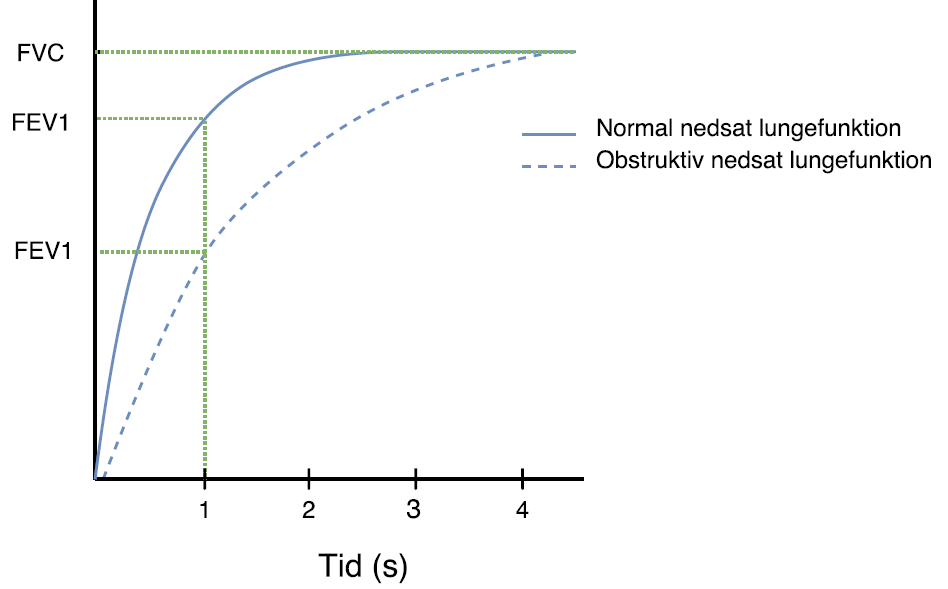
\includegraphics[width=0.8\textwidth]{figures/FEV}
\caption{Spirometrimålinger for patienter med normal og obstruktiv nedsat lungefunktion. Revideret\cite{Basisbogen2016}.}
\label{fig:FEV}
\end{figure} 

\noindent
Det fremgår af \autoref{fig:FEV}, at der ved obstruktivt og restriktiv nedsat lungefunktion er et fald i FEV1 samt FVC. Der udføres ligeledes en reversibilitetstest for at sikre, at patienter ikke lider af differentialdiagnosen astma. Disse patienter gives broncodilatorer, som hos astmapatienter vil forbedre spirometrimålingen, mens lungefunktionen for KOL-patienter forbliver uændret.\cite{Basisbogen2016, Sundhed2013} 
For at undersøge KOL og patienters komorbiditeter undersøges foruden lungefunktionsundersøgelser også BMI, røntgen af thorax, EKG-målinger og blodprøver \cite{Sundhed2013}. 
%Med tiden kan symptomerne på KOL forværres, og der skal mindre fysisk aktivitet til for at udløse åndenød. \cite{Basisbogen2016}
\subsubsection{Klassifikation af KOLs sværhedsgrad} \label{sec:klassifikation}
Sværhedsgraden af KOL vurderes på baggrund af patienters symptomer, egne erfaringer og livskvalitet. Denne vurderes ud fra Medical Research Council åndenødsskala (MRC) eller Chronic obstructive pulmonary disease Assessment Test (CAT). Patienter kan efterfølgende inddeles i klassifikationer med udgangspunkt i MRC, CAT eller ved spirometrimålinger.\cite{Basisbogen2016}

 
MRC-skalaen er en skala fra $1$ til $5$, hvor patienter vurderer mængden af aktivitet, som de kan udføre i forhold til åndenød. Skalaen fremgår af \autoref{tab:MRC}, hvor $1$ svarer til, at patienter først oplever åndenød ved meget anstrengelse, og $5$ svarer til, at patienter oplever åndenød ved meget lav fysisk aktivitet.\cite{Basisbogen2016}

\begin{table} [H]
\centering
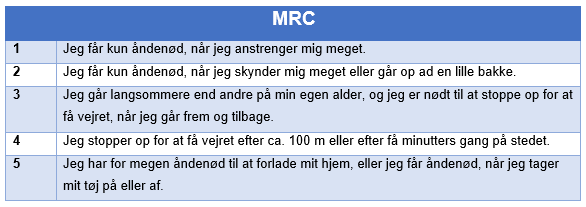
\includegraphics[width=0.9\textwidth]{figures/MRC}
\caption{MRC er en skala fra $1$ til $5$. Patienter, der oplever åndenød ved meget anstrengelse vurderes til $1$, mens patienter, der oplever åndenød ved lav aktivitet vurderes til $5$ på MRC-skalaen. Revideret\cite{Basisbogen2016}.}
\label{tab:MRC}
\end{table} 

\noindent
En anden metode til at vurdere symptomerne ved KOL er ved hjælp af CAT-spørgeskema. Her vurderes otte udsagn fra en skala fra $0$ til $5$, hvor ingen symptomer angives $0$. Ud fra de otte udsagn opnås en samlede score, jo højere den samlede score er, desto værre opleves patienters symptomer. Af \autoref{fig:CAT} ses CAT-spørgeskema til vurdering af symptomer.\cite{dsam2016,Basisbogen2016}

\begin{figure} [H]
\centering
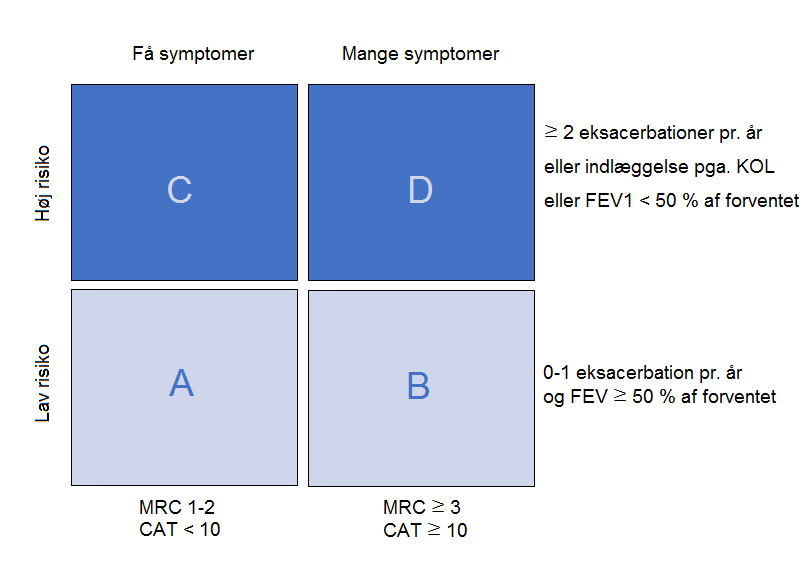
\includegraphics[width=0.5\textwidth]{figures/CAT}
\caption{CAT er et spørgeskema, hvor patienter vurderer graden af deres symptomer ud fra otte udsagn på en skala fra $0$ til $5$. Ingen symptomer svarer til $0$. Patienter opnår en samlede score, jo højere den samlede score er, desto værre opleves patienters symptomer. Revideret\cite{Basisbogen2016}.}
\label{fig:CAT}
\end{figure} 

\noindent
Ud fra MRC-skalaen eller CAT-spørgeskemaet samt lungefunktionstest og antallet af eksacerbationer det seneste år kan KOL-patienter kategoriseres. Patienterne kategoriseres i A, B, C eller D, hvor D er patienter i høj risiko og med mange symptomer. Kategoriseringen fremgår af \autoref{fig:KAT}.

\begin{figure} [H]
\centering
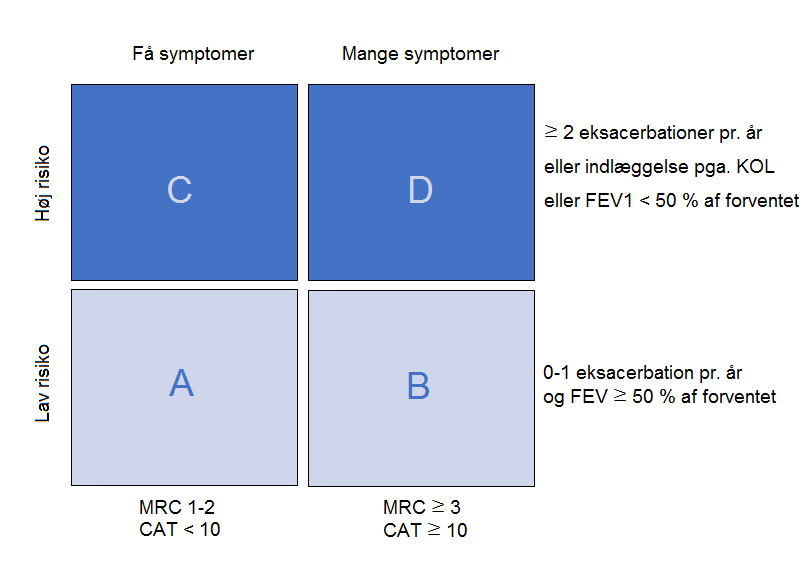
\includegraphics[width=0.8\textwidth]{figures/KAT}
\caption{KOL-patienter kategoriseres i fire kategorier herunder A, B, C og D. A og B inddeles i lav risiko, mens C og D er i høj risiko. Revideret\cite{Basisbogen2016}.}
\label{fig:KAT}
\end{figure} 
 
\noindent
Udover ABCD-kategoriseringen kan sværhedsgraden af KOL udelukkende bestemmes ud fra spirometrimålinger.  Sværhedsgraden er klassificeret ud fra retningslinjer opstillet af the Global Initiative for Chronic Obstructive Lung Disease (GOLD).\cite{dsam2016} Lungefunktionen vurderes på baggrund af FEV$1$ i \% af den forventede lungekapacitet, hvoraf det inddeles i fire stadier. Disse fremgår af \autoref{tab:GOLD}.

\begin{table} [H]
\centering
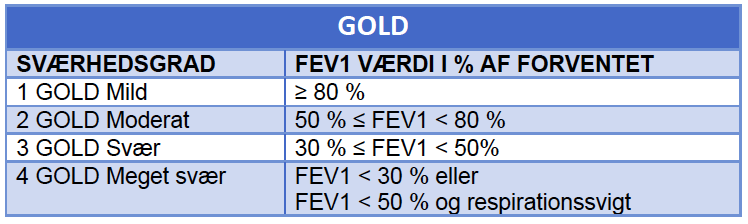
\includegraphics[width=0.8\textwidth]{figures/GOLD}
\caption{GOLD er inddelt efter sværhedsgraderne $1$ til $4$ herunder mild, moderat, svær og meget svær. Patienter, der har over $80~\%$ af forventet lungekapacitet klassificeres som $1$ GOLD mild, mens patienter med under $30~\%$ eller over $50~\%$ af forventet lungekapacitet samt respirationssvigt klassificeres som $4$ GOLD meget svær. Revideret\cite{Basisbogen2016}.}
\label{tab:GOLD}
\end{table} 

\subsection{Behandling} \label{sec:behandling}
Det er ikke muligt at helbrede patienter med KOL, da KOL er en kronisk lungesygdom. Dog er det muligt at forhindre udviklingen af KOL samt lindre symptomerne, hvilket kan opnås ved tobaksafvænning, fysisk aktivitet, kostvejledning og medicin.\cite{Basisbogen2016} 

KOL-patienter med sekretproblemer tilbydes continous positive airway pressure (CPAP) eller positive expiratory pressure (PEP-fløjte) og broncodilaterende inhalationsbehandling efter behov og ud fra graden KOL. Yderligere kan antiinflammatorisk behandling gives til patienter med hyppige eksacerbationer.\cite{Basisbogen2016}

Da den tabte lungefunktion ikke kan genvindes, rådes patienterne til ophøre tobaksrygning eller det der kan være årsagen til KOL f.eks. dårligt arbejdsmiljø, hurtigst muligt for således at bibeholde den nuværende lungefunktion \cite{Basisbogen2016}. Det fremgår af \autoref{fig:fletcher}, hvordan tobaksrygning kan påvirke lungefunktionen over tid. 

\begin{figure} [H]
\centering
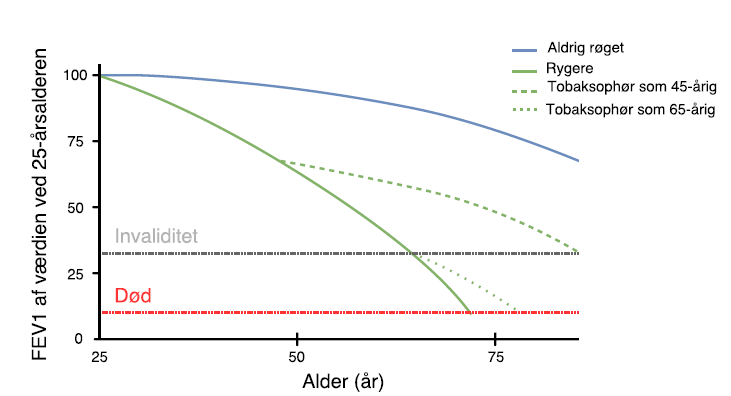
\includegraphics[width=1\textwidth]{figures/fletcher}
\caption{Fletcher-kurve, som viser faldet af FEV1 over tid for henholdsvis rygere, ikke-rygere og rygere med tobaksophør i $45$- og $65$-årsalderen. Revideret\cite{Basisbogen2016}.}
\label{fig:fletcher}
\end{figure} 

\noindent
Det ses af \autoref{fig:fletcher}, at tobaksrygning medvirker til et accelererende tab af FEV1, og dermed udsigt til kortere levetid. På trods af tobaksophør genoprettes FEV$1$ ikke, dog bremses det accelerende tab af FEV$1$ til det normale aftag.\cite{dsam2016}

\subsection{Prognose}
KOL-patienter med eksacerbationer har efter indlæggelse en dødelighed på næsten $10$~$\%$ i løbet af den første måned. Dødeligheden ligger på omkring $64$ per $100.000$ per år for mænd og $54$ per $100.000$ per år for kvinder.
Udviklingen, hvormed sygdommen progredierer for KOL-patienter er specielt afhængig af, hvorvidt patienter ophører eksponering til den udløsende faktor for eksempel tobaksophør. Det er derfor vigtigt at få en tidlig diagnosticering således, at patienter hurtigt kan få hjælp.\cite{dsam2016}
%Derudover har et studie vist, at KOL-patienter, der er i stadie $4$ i GOLD-klassificeringen, har lav funktionalitet og livskvalitet, som bliver værre med tiden og ved fremkomst af flere symptomer til sygdommen. \cite{Habraken2011}


\section{Rehabilitering}
Da KOL er kronisk lungesygdom, hvorved den tabte lungefunktion ikke kan genoprettes, tilbydes KOL-patienter rehabilitering med henblik på at mindske deres symptomer. 

I Danmark henvises KOL-patienter til rehabilitering fra praktiserende læge eller hospital. Rehabilitering forløber typisk over $8$ ugers periode på et sundhedscenter eller på et hospital. KOL-patienter møder til træning $1$-$2$ gange om ugen, de resterende dage vil patienten kunne udføre de fremviste øvelser hjemme. \cite{McCarthy2015}[lunge.dk/rehabilitering] 

Individuel rehabilitering anses som værende fundamental for KOL-patienter, hvor forløbet tilpasses i forhold til patienternes behov med henblik på at opnå det bedste udbytte af rehabiliteringen \cite{McCarthy2015,Habraken2011}[sundkol2015]. Ligeledes vurderes rehabiliteringen på baggrund af graden af KOL, da KOL fremkommer i flere grader samt med varierende progression \cite{McCarthy2015}. 

Rehabiliteringen kan give patienter bedre mulighed for deltagelse i hverdagen, såfremt patienters tilstand tillader det. \cite{McCarthy2015,Habraken2011} [sundkol2015] Opfølgninger kan foretages efter rehabiliteringsforløb er afsluttet, for at undersøge om patienter opretholder de gavnlige effekter. [lunge.dk/rehabilitering]


\subsection{Rehabiliteringsforløbet}
Rehabiliteringsforløbet fokuserer på tobaksafvænning, fysisk træning, kendskab til sygdommen samt ernæringsvejledning. \cite{McCarthy2015,Habraken2011} [sundkol2015] 

Tobaksafvænning er, som beskrevet i \autoref{sec:behandling}, et relevant element i forhold til at begrænse udviklingen af sygdommen og bevare mest mulig lungefunktion. Den fysiske træning, der udføres under rehabiliteringen, medvirker til, at patienter kan opnå et bedre udbytte af den resterende lungefunktion, samt opnå et bedre fysisk funktionsniveau [sundkol2015]. 
Træningen vil ligeledes modvirke eventuelle følger ved KOL, da fysisk træning øger muskelfunktionen samt udsætter træthed, hvilket medfører forøget aktivitetstolerance \cite{McCarthy2015}. Dog kan den fysiske træning resultere i åndenød hos KOL-patienter, der kan forstærkes, hvis patienter påvirkes af angst som følge af åndenød. Dette kan betyde, at KOL-patienter afholder sig fra fysisk træning på grund af frygten for angst. \cite{McCarthy2015} [sundKOL2015]. 

Et led i rehabiliteringen er ligeledes, at patienter opnår viden indenfor sygdomshåndtering, der omhandler kendskab til og forebyggelse af sygdommen, livsstilsændringer samt håndtering af eksacerbationer\cite{McCarthy2015} [sundKOL2015]. Her fokuseres blandt andet på de gavnlige effekter ved tobakophør og regelmæssig fysisk aktivitet, samt hvornår og hvordan eventuel medicin skal indtages. Patienten vil yderligere blive introduceret til energibesparende strategier og vejrtrækningsøvelser \cite{McCarthy2015} [sundkol2015].   


\section{Problemformulering}
\textit{Hvordan udvikles en app til at vejlede og motivere KOL-patienter til hjemmetræning i forlængelse af rehabiliteringsforløb med henblik på at mindske symptomer forbundet med KOL? }

%-----------------------Problemanalyse---------------------------
\chapter{Metode II}
***    Mangler indledning (evt. hvorfor vi bruger OOP)   *****

\section{Objektorienteret programmering}
Objektorienteret programmering er et programmeringsparadigme, som anvendes til at analysere, designe, implementere samt udvikle app's. Hyppige termer inden for objektorienteret programmering er blandt andet objekter, klasser, indkapsling, nedarvning og polymorfi.\cite{Stefanov2013,Brahma2015}

I objektorienteret programmering opdeles programmeringskoden i klasser, hvor hver klasse fungerer som en opskrift for et objekt. Hvert objekt er en instans af en bestemt klasse, hvor en klasse kan være bygget op omkring en eller flere instanser. De forskellige objekter repræsenterer hver sin del af app'en og indeholder data og logik. Derudover har objekterne mulighed for at kommunikere mellem hinanden. Objekter er karakteriseret ud fra deres egenskaber, og deres funktioner er beskrevet ved metoder.\cite{Stefanov2013,Brahma2015} Eksempler på egenskaber og metoder fremgår af \autoref{tab:objekt}. 

\begin{table}[H]
\centering
\begin{tabular}{|l|l|}
\hline
\textbf{Egenskaber} & \textbf{Metoder} \\ \hline
\begin{tabular}[c]{@{}l@{}}Navn \\ Køn\\ Alder\\ Højde \\ Vægt\end{tabular} & \begin{tabular}[c]{@{}l@{}}Gå\\ Løbe\\ Hoppe\\ Sove\\ Tale\end{tabular} \\ \hline
\end{tabular}
\caption{Objekter karakteriseres ud fra deres egenskaber som for eksempel navn, mens metoder beskriver deres funktion som for eksempel sove.}
\label{tab:objekt}
\end{table}

\noindent
Objektorienteret programmering består af tre grundprincipper, herunder indkapsling, nedarvning og polymorfi. Indkapsling er en illustration af, at objekter både indeholder egenskaber og metoder. Egenskaber opbevarer data, mens metoder anvendes til at behandle data. Indkapsling kan både have synlige og skjulte informationer. Synlig information udgør  ofte grænsefladen, såsom knapper og display, mens skjult information kan være implementeringen af grænsefladen. Dette gør sig også gældende for objekter, hvilket defineres som public eller private. Ved public har alle objekter adgang til metoderne, mens private kun er metoder med samme objekt, der kan tilgå denne. Nedarvning betyder, at et objekt kan arve data og funktioner fra et andet objekt. Dette muliggør, at objektet kan udvides med ekstra data og funktioner. Polymorfi giver mulighed for, at to klasser kan have samme grænseflade. Denne er defineret ved nedarvningen.\cite{Stefanov2013}

\section{Unified Modellig Language}
Til at dokumentere den objektorienteret programmering og udvikling af systemet i denne rapport, anvendes standarden Unified Modelling Language (UML). Dette er valgt for at fremstille software analysen af systemet, samt dets design. Hertil anvendes udvalgte UML modeller: Use-case, Aktivitets og klasse-diagrammer. 

\subsection{Use-case diagrammer} 
Use-case diagrammer benyttes til at illustrere aktørernes interaktion med et 'system', samt hvordan forskellige use-cases interagere mellem hinanden. Dertil er use-case diagrammet med til at repræsentere funktionelle krav for systemet. Et simpelt eksempel ses af \autoref{fig:use_case} 

\begin{figure} [H]
\centering
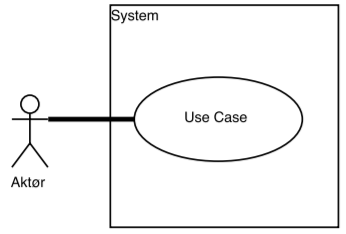
\includegraphics[width=0.5\textwidth]{figures/USE_CASE2}
\caption{Simpelt use-case diagram.}
\label{fig:use_case}
\end{figure}

Af \autoref{fig:xx2} ses aktørens interaktion med use-case visualiseret som en streg mellem de to. I et use-case diagram vil aktøren definere en person/rolle, objekt, eller anden given genstand der kan tilgå system funktionaliteter. Hertil vil den enkelte use-case beskrive en handling eller funktionalitet i systemet. 


\subsection{Aktivitetsdiagrammer}
Til at beskrive komplekse use-cases eller klasse metoder anvendes aktivitetsdiagrammer. Dette er for at give overblik flowet ved at beskrive aktiviteterne i den givne funktion eller metode.     

Såfremt der i et aktivitetsdiagram anvendes et 'brille' symbol, indikerer dette at den aktivitet i sig selv er kompleks og er beskrevet i et særskilt aktivitetsdiagram.  

\subsection{Klassediagrammer}
Klassediagrammet vil blive anvendt som et redskab til at designe og give overblik over de forskellige klasser. Hertil vil relationerne mellem de forskellige klasser blive tydeliggjort ved anvendelse af tilhørende symbolisering: nedarvning, association, aggregation, composition mm. Som det ses af \autoref{fig:klassediagram} beskrives hver klasse ud fra et unik klassenavn hvor der yderligere kan tildes attributter og metoder til den givne klasse.  

\begin{figure} [H]
\centering
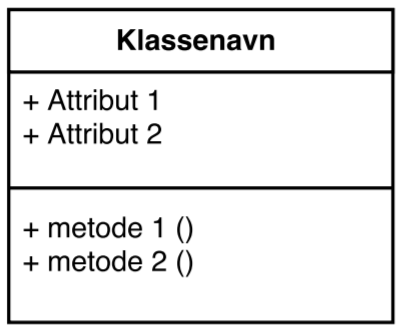
\includegraphics[width=0.5\textwidth]{figures/klassediag}
\caption{}
\label{fig:klassediagram}
\end{figure}
\section{Unified Process} \label{sec:UP}
En objektorienteret softwareudviklingsproces er Unified Process (UP), som definerer hvem, hvad, hvornår og hvordan softwaren udvikles. UP er bygget om omkring iterationer, hvor softwareudviklingsprocessen deles op i mindre projekter. Dette gøres da det forventes, at fejl opdages hurtigere og er lettere at løse, hvilket ofte medfører, at projekter gennemføres med succes. Hvert projekt er en iteration og opdeles i arbejdsmængder, såsom krav, analyse, design, implementering og test. Denne arbejdsmængde opdeles yderligere i fire faser, herunder opstart, udarbejdelse, konstruktion og overgang, hvor hver fase afsluttes med en milepæl. Hver fase har en eller flere iterationer. Antallet af iterationer afhænger af projektets størrelse. De forskellige faser overlappes i forbindelse med projektets fremskreden og arbejdsmængden ændres.\cite{Arlow2002} Opdeling af projektet og arbejdsmængden ud fra UP fremgår af \autoref{fig:UP}

\begin{figure} [H]
\centering
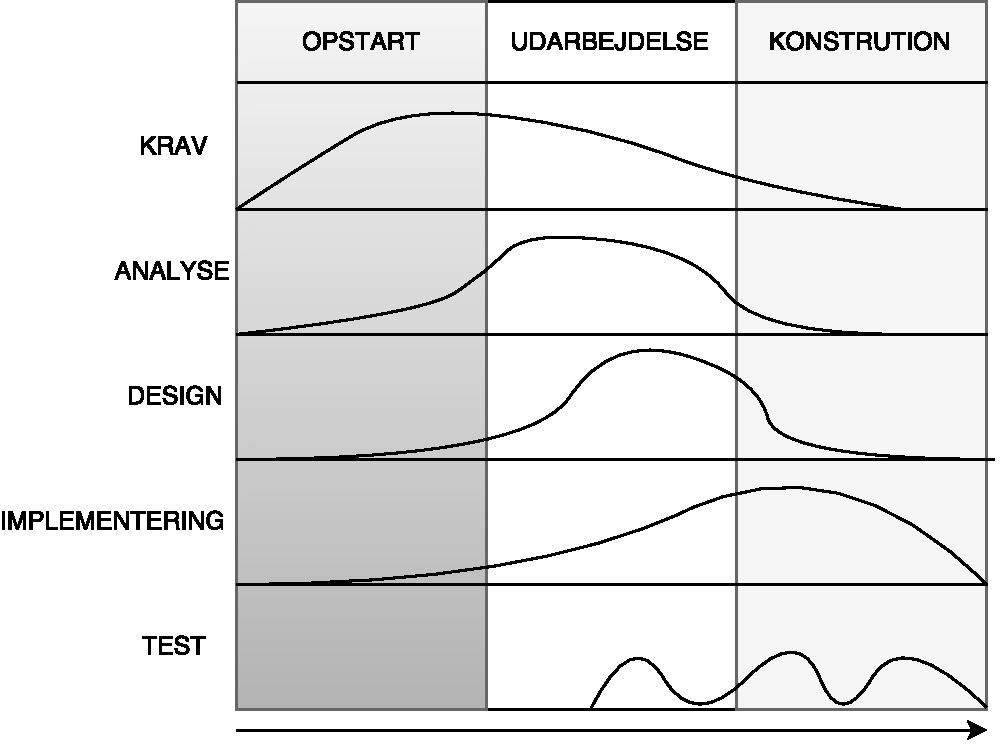
\includegraphics[width=0.8\textwidth]{figures/UP}
\caption{UP struktur. X-aksen viser tiden over projektet opdelt i opstart, udarbejdelse og konstruktion. Y-aksen viser projektets faser, herunder krav, analyse, design, implementering og test. Kurverne viser arbejdsmængden. Revideret \cite{Arlow2002}}
\label{fig:UP}
\end{figure} 

\noindent
Af \autoref{fig:UP} fremgår softwareprocesudviklingen i dette projekt. Opstart og udarbejdelse anvendes med henblik på den senere implementering i konstruktionsfasen. Den sidste fase, overgang, er udeladt af dette projekt, da der kun udvikles en prototype. \fxnote{Skal ændres lidt til hvis vi oplever fejl}

%\section{Software Development Lifecycle}
%Software development lifecycle (SDLC) er en række trin, der kan følges, til udvikling af softwaresystemer for at skabe struktur over arbejdsprocessen. Der er forskellige typer af modeller indenfor SDLC, og dermed forskellige fremgangsmåder for, hvordan processen i softwareudviklingen kan foregå. Eksempler på SDLC-modeller, som anvendes i virksomheder, er vandfaldsmodellen, spiralmodellen og V-modellen. En typisk SDLC-model indeholder stadierne; planlægning, definering, design, implementering, test og brug af systemet.\cite{Jain2011}
%
%\subsection{Vandfaldsmodel} \label{sec:vandfald}
%Vandfaldsmodellen er den ældste og mest brugte SDLC model til udvikling af softwaresystemer. Modellen følger fem faser; analyse og kravspecifikationer, design, implementering, test samt vedligeholdelse. Disse faser gennemgås og dokumenteres enkeltvis førend næste fase påbegyndes. Dette bidrager til at sikre kvaliteten af systemudviklingen. Ved vandfaldsmodellen kan der dog også opstå problematikker i forhold til fejl. Disse fejl kan eksempelvis opstå i første fase, men først opdages i fjerde fase, hvorfor faserne derved skal gennemgås igen.\cite{Alshamrani2015,Bassil2012} Af \autoref{fig:vandfaldsmodel} fremgår vandfaldsmodellen med de fem faser. 
%
%\begin{figure} [H]
%\centering
%\includegraphics[width=0.8\textwidth]{figures/vandfaldsmodel}
%\caption{Vandfaldsmodellens fem faser bestående af analyse og kravspecifikation, design, implementering, test samt vedligeholdelse. Revideret \cite{Alshamrani2015,Bassil2012}.}
%\label{fig:vandfaldsmodel}
%\end{figure} 
%
%\noindent
%Den første fase, analyse og kravspecifikationer, er en omfattende analyse samt beskrivelse af systemets formål. Herunder opstilles funktionelle og non-funktionelle krav, der beskriver, hvilke funktioner samt begrænsninger systemet burde have. Under første fase udarbejdes ligeledes use-case diagrammer i sammenhæng med de funktionelle krav. Efter analyse og kravspecifikationer forekommer designet af systemet. I denne fase planlægges og designes en softwareløsning baseret ud fra første fases kravspecifikationer. Herunder udvælges blandt andet algoritme design, software arkitektur design, databasedesign samt definition af datastruktur. Tredje fase indebærer implementeringen. Denne fase har til formål at implementere og konvertere de opstillede kravspecifikationer samt design fra tidligere faser til et system. Denne konvertering foregår gennem programmering. Den fjerde fase omhandler test og kontrol af softwareløsningen i forhold til de opstillede kravspecifikationer. Vedligeholdelsesfasen, der er den sidste fase, indebærer eventuelle ændringer og forbedringer af softwaresystemet efter det er frigivet.\cite{Alshamrani2015,Bassil2012}










%%-----------------------System udvikling-------------------------
\part{Problemløsning}
\chapter{Systemanalyse} \label{cha:analyse}
I dette kapitel beskrives funktionaliteten af den ønskede app. På baggrund af dette opstilles funktionelle samt non-funktionelle krav. Herefter er systemet beskrevet ved hjælp af et use case diagram, hvortil de enkelte funktionaliteter er beskrevet yderligere. 

\section{Systembeskrivelse} \label{sec:systembeskrivelse}
I dette projekt udvikles en app, der har til formål at hjælpe KOL-patienter til at opretholde regelmæssig motion efter et endt rehabiliteringsforløb. App'en skal kunne håndtere forskellige træningsformer herunder konditions- samt styrketræning og vejrtrækningsøvelser, hvilket alle har symptomreducerende effekt, jf. \autoref{sec:rehabilitering}. Ligeledes skal app'en kunne håndtere forskellige træningstyper, som for eksempel gå, løbe eller cykle.

KOL-patienter introduceres samt registreres i app'en i forbindelse med deres rehabiliteringsforløb. 
Dette skal sikre, at det kun er KOL-patienter, der er tilmeldt rehabiliteringshold, som kan anvende app'en til træning. Ved registrering oprettes KOL-patienter med medlemsID, fornavn, efternavn samt adgangskode.  

Der er forskel på, hvor meget fysisk aktivitet KOL-patienter kan udføre, og der skal derved være forskel i varighed af den træning som app'en foreslår. Dertil skal app'en kunne tilpasse træningsniveau ud fra den enkelte patients parametre. Disse parametre består af kategoriseringen af KOL-patienter efter ABCD, jf. \autoref{cha:problemanalyse}, daglige helbredstilstande, der skal tage højde for dag til dag variationer samt tidligere evalueringer fra lignende træningstype. Dette medvirker til, at app'en er henvendt specifik til KOL-patienter i modsætning til andre træningsapp's, der henvender sig til hele befolkningen. 

Under selve træningen monitoreres træningen ved brug af timer og GPS. Monitoreringen er med til at vejlede patienten til at følge det valgte træningsniveau. 

For at hjælpe KOL-patienter med vedligeholdelse af den daglige træning skal app’en virke motiverende for patienterne. Dette gøres blandt andet ved, at KOL-patienter kan opnå virtuelle belønninger ved at udføre gentagne eller forskellige træningsformer. Desuden skal app'en informere, hvis KOL-patienter ikke har udført træning med app'en i længere tid. \citep{Gade2007, Tricomi2016}

Som nævnt i afsnit \ref{sec:efterRehabilitering}, er det sociale fællesskab en væsentlig faktor for at opretholde resultaterne fra rehabiliteringsforløb. Dette gøres ved, at KOL-patienter kan følge og tilgå andre KOL-patienters virtuelle belønninger, hvormed dette motiverer patienterne til vedligeholdelse af den forbedrede livsstil. Derudover skal sundhedsfagligt personale kunne tilgå KOL-patienters resultater i en database, så de kan følge med i patienters udvikling. De har herved mulighed for at informere patienter om deres indsats, hvilket ligeledes kan have en motiverende effekt.\citep{Gade2007, Tricomi2016}


\section{Kravspecifikationer} \label{sec:funktionellekrav}
På baggrund af systembeskrivelsen er funktionelle og non-funktionelle krav til app'en opstillet. De funktionelle krav beskriver, hvilke funktionaliteter app'en skal have. De non-funktionelle krav er opstillet ud fra overbevisningen om, at det ikke er krav til systemets funktionalitet, men er relevant i relation til brugervenlighed og brugeroplevelse. 


\subsubsection{Funktionelle krav}

\noindent 
\begin{itemize}
\item Brugere skal kunne oprettes i en database
	\\
	\textit{Dette er nødvendigt for, at brugere kan anvende app'en}
	\item Systemet skal kunne gemme og hente data i en database
\\
\textit{Dette er nødvendigt for, at brugere kan tilgå brugerdata}
\item Brugere skal kunne logge ind med et personligt medlemsID og adgangskode
	\\
	\textit{Dette er nødvendigt for at tilgå og sikre, at brugere har deltaget i et rehabiliteringsforløb samt adskille brugernes data}
\item Systemet skal kunne kategorisere brugere i ABCD på baggrund af CATscore og  antallet af indlæggelser på grund af KOL. 
	\\
	\textit{Dette er nødvendigt for at kunne tilpasse træningen efter den enkelte bruger}
\item Brugere skal kunne angive deres daglige helbredstilstand 
	\\
\textit{Dette er nødvendigt for tage højde for daglige variationer og derved tilpasse træningen for den enkelte bruger}
\item Systemet skal kunne måle tid og afstand
	\\
\textit{Dette er nødvendigt for at monitorere træningen}
\item Brugere skal kunne evaluere hver træning
	\\
\textit{Dette er nødvendigt for at tilpasse træningen efter den enkelte bruger}		
\item Systemet skal kunne sende en notifikation, hvis brugere ikke har trænet før klokken 15. 
	\\
	\textit{Dette er nødvendigt for at kunne motivere brugere til at udføre træning}
	
	\item Systemet skal kunne give virtuelle belønninger 
	\\
	\textit{Dette er nødvendigt for at kunne motivere brugere til at udføre træning}
\item Brugere skal kunne følge andre brugere 
	\\
	\textit{Dette er nødvendigt for at skabe fællesskab samt gøre det muligt for brugere at tilgå hinandens virtuelle belønninger, hvilket skal øge brugeres motivation}
\item Brugere skal kunne redigere deres adgangskode
	\\
	\textit{Dette er nødvendigt for, at brugere skal kunne gøre deres adgangskode personlig}
\item Brugere skal kunne log ud af app'en
	\\
	\textit{Dette er nødvendigt for sikre brugerens individuelle data}
\end{itemize}


\subsubsection{Non-funktionelle krav}

\begin{itemize}
\item Systemet skal visualiseres på en smartphone eller tablet med android 
\item Systemet skal være brugervenligt
	\\
	\textit{Dette er nødvendigt for at sikre let orientering i app'en}
\end{itemize}



%I dette kapitel opstilles krav til en app for at kunne udvikle et system, der opfylder problemformuleringen. Først beskrives systemet ud fra, hvad der ønskes, at det skal kunne, hvorudfra funktionelle og non-funktionelle krav opstilles.
%
%\section{Systembeskrivelse} \label{sec:systembeskrivelse}
%I dette projekt udvikles en app, der har til formål at kunne anvendes af KOL-patienter som et redskab til opretholdelse af de gavnlige effekter, der opnås under rehabiliteringsforløb.
%
%Under rehabiliteringsforløb lærer KOL-patienter forskellige træningsøvelser, som har en symptomlindrende effekt, jf. afsnit \ref{sec:rehabilitering}. App’en skal foreslå træningsøvelser, som KOL-patienterne kan udføre, så de fortsat får udført fysisk aktivitet i hjemmet efter endt rehabiliteringsforløb. Disse træningsøvelser skal udvælges på baggrund af de øvelser, der udføres under rehabiliteringsforløb, således at KOL-patienter allerede har erfaringer og kendskab til de øvelser, som app’en foreslår.
%Der er forskel på, hvor meget fysisk aktivitet forskellige KOL-patienter kan udføre, og der er derved forskel i varighed og intensitet af de træningsøvelser. For at tage højde for dette under valg af træningsøvelser, udvælges øvelserne på baggrund af den enkelte patients sværhedsgrad af KOL. Sværhedsgraden bestemmes ud fra ABCD-kategoriseringen, jf. \ref{sec:klassifikation}, som patienter skal angive, når de registreres som brugere første gang app'en anvendes. 
%For at reducere risikoen for, at KOL-patienter får negative oplevelser ved anvendelse af app’en, hvilket eksempelvis ville kunne ske, hvis der foreslås træningsøvelser på for højt niveau i forhold til patientens tilstand, skal app’en kunne tage højde for de daglige variationer i patientens sygdom. Dette imødekommes ved, at patienter angiver sit helbred til app'en den pågældende dag.
%Ud fra dette tilpasses træningsøvelserne, som KOL-patienterne bliver foreslået. Efter en udført
%træningssession skal patienten evaluere træningen i forhold til sværhedsgraden af træningen,
%så denne evaluering kan medtages i udvælgelsen af den efterfølgende dags anbefalede træning. Herved kan træningen tilpasses den enkelte KOL-patients tilstand.
%For at hjælpe KOL-patienter med vedligeholdelse af den daglige træning skal app’en virke motiverende for patienterne. Dette gøres blandt andet ved at gøre det muligt for KOL-patienter at følge sin egen udvikling via app’en. App’en skal desuden gøre KOL-patienter opmærksom på, hvis de ikke har været aktive på app'en i længere tid. For at øge motivation hos KOL-patienter skal de derudover kunne opnå virtuelle belønninger ved at udføre træningssessioner.
%
%Som nævnt i afsnit \ref{sec:efterRehabilitering}, er det sociale fællesskab en væsentlig faktor i opretholdelse af resultaterne fra rehabiliteringsforløb. Ved at indføre denne faktor i app’en kan dette være med til at motivere KOL-patienter til vedligeholdelse af den forbedrede livsstil. Dette gør det desuden muligt at gøre patienter opmærksom på, at andre brugere af app’en har udført en træningssession, hvilket kan virke motiverende.
%Sundhedsfagligt personale skal kunne tilgå KOL-patienters resultater, så de kan følge med i udviklingen. De har herved mulighed for at informere patienter om, hvorvidt de træner for lidt eller om de gør et godt arbejde, hvilket også kan have en motiverende effekt på KOL-patienter.
%
%\subsection{Funktionelle krav}
%Ud fra informationer fundet gennem problemanalysen i \autoref{cha:problemanalyse} og beskrivelsen af systemet i \autoref{sec:systembeskrivelse} er nedenstående funktionelle krav opstillet. 
%  
%\begin{itemize}
%\item Systemet skal kunne oprette forbindelse til databasen
%	\\
%	\textit{Dette er nødvendigt for at gemme, hente og redigere data}
%
%\item Systemet skal kunne gemme data i databasen
%	\\
%	\textit{Dette er nødvendigt for at tilgå tidligere resultater}
%
%\item Systemet skal kunne hente data fra databasen
%	\\
%	\textit{Dette er nødvendigt for at tilgå tidligere resultater for både patienter og sundhedspersonale}	
%	
%\item Systemet skal kunne oprette nye brugere 
%	\\
%	\textit{Dette er nødvendigt for, at flere KOL-patienter kan anvende app'en}
%
%\item Systemet skal kunne redigere brugeroplysninger
%	\\
%	\textit{Dette er nødvendigt, hvis patienters tilstand ændres}
%
%\item Systemet skal have en login og logout funktion
%	\\
%	\textit{Dette er nødvendigt for at sikre patienters individuelle data}
%
%\item Systemet skal kunne kategorisere og vurdere  KOL-patienters helbredstilstand 
%	\\
%	\textit{Dette er nødvendigt for at kunne tilpasse træningssæt efter den enkelte KOL-patient}
%
%\item Systemet skal kunne sende notifikationer og give virtuelle belønninger 
%	\\
%	\textit{Dette er nødvendigt for at kunne motivere patienter til at udføre træning}
%
%\item Systemet skal kunne interagere med andre KOL-patienter
%	\\
%	\textit{Dette er nødvendigt for motivering mellem KOL-patienter samt skabe fællesskab}
%	\\
%	\textit{Dette er nødvendigt for at patienter kan tilgå hinandens virtuelle belønninger}
%	\\
%	\textit{Dette er nødvendigt for at kunne give notifikationer, hvis andre patienter træner}
%
%\end{itemize}
%
%\subsection{Non-funktionelle krav}
%De non-funktionelle krav er opstillet ud fra en den overbevisning, at dette ikke er krav til systemets funktionalitet, men stadig er relevant i relation til den bedste udbredelse, brugervenlighed og brugeroplevelse. 
%
%\begin{itemize}
%\item Systemet skal kunne fungere på en smartphone eller tablet 
%\item Systemet skal være brugervenligt
%	\\
%	\textit{Dette er nødvendigt, da KOL-patienter ofte er ældre}
%	
%\item Systemet skal tilgås med et medlemsnummer, navn og kodeord
%	\\
%	\textit{Dette er nødvendigt for at sikre, at KOL-patienter har deltaget i et rehabiliteringsforløb}
%	\\
%	\textit{Dette er nødvendigt for at adskille patienters data}
%\end{itemize}
\section{Use case} \label{sec:usecase} 
På baggrund af systembeskrivelsen samt opstillede krav er der udarbejdet et use case diagram, der beskriver app'ens funktioner. Af use case diagrammet på \autoref{fig:usecase} ses systemet, app til KOL-patienter, samt de forskellige use cases og aktører, der kan interagere med systemet. KOL-patienten er den primære aktør, som kan tilgå alle use cases. Målinger, database, sundhedspersonale og andre KOL-patienter er sekundære aktører og kan kun tilgå enkelte use cases. 

\begin{figure} [H]
\centering
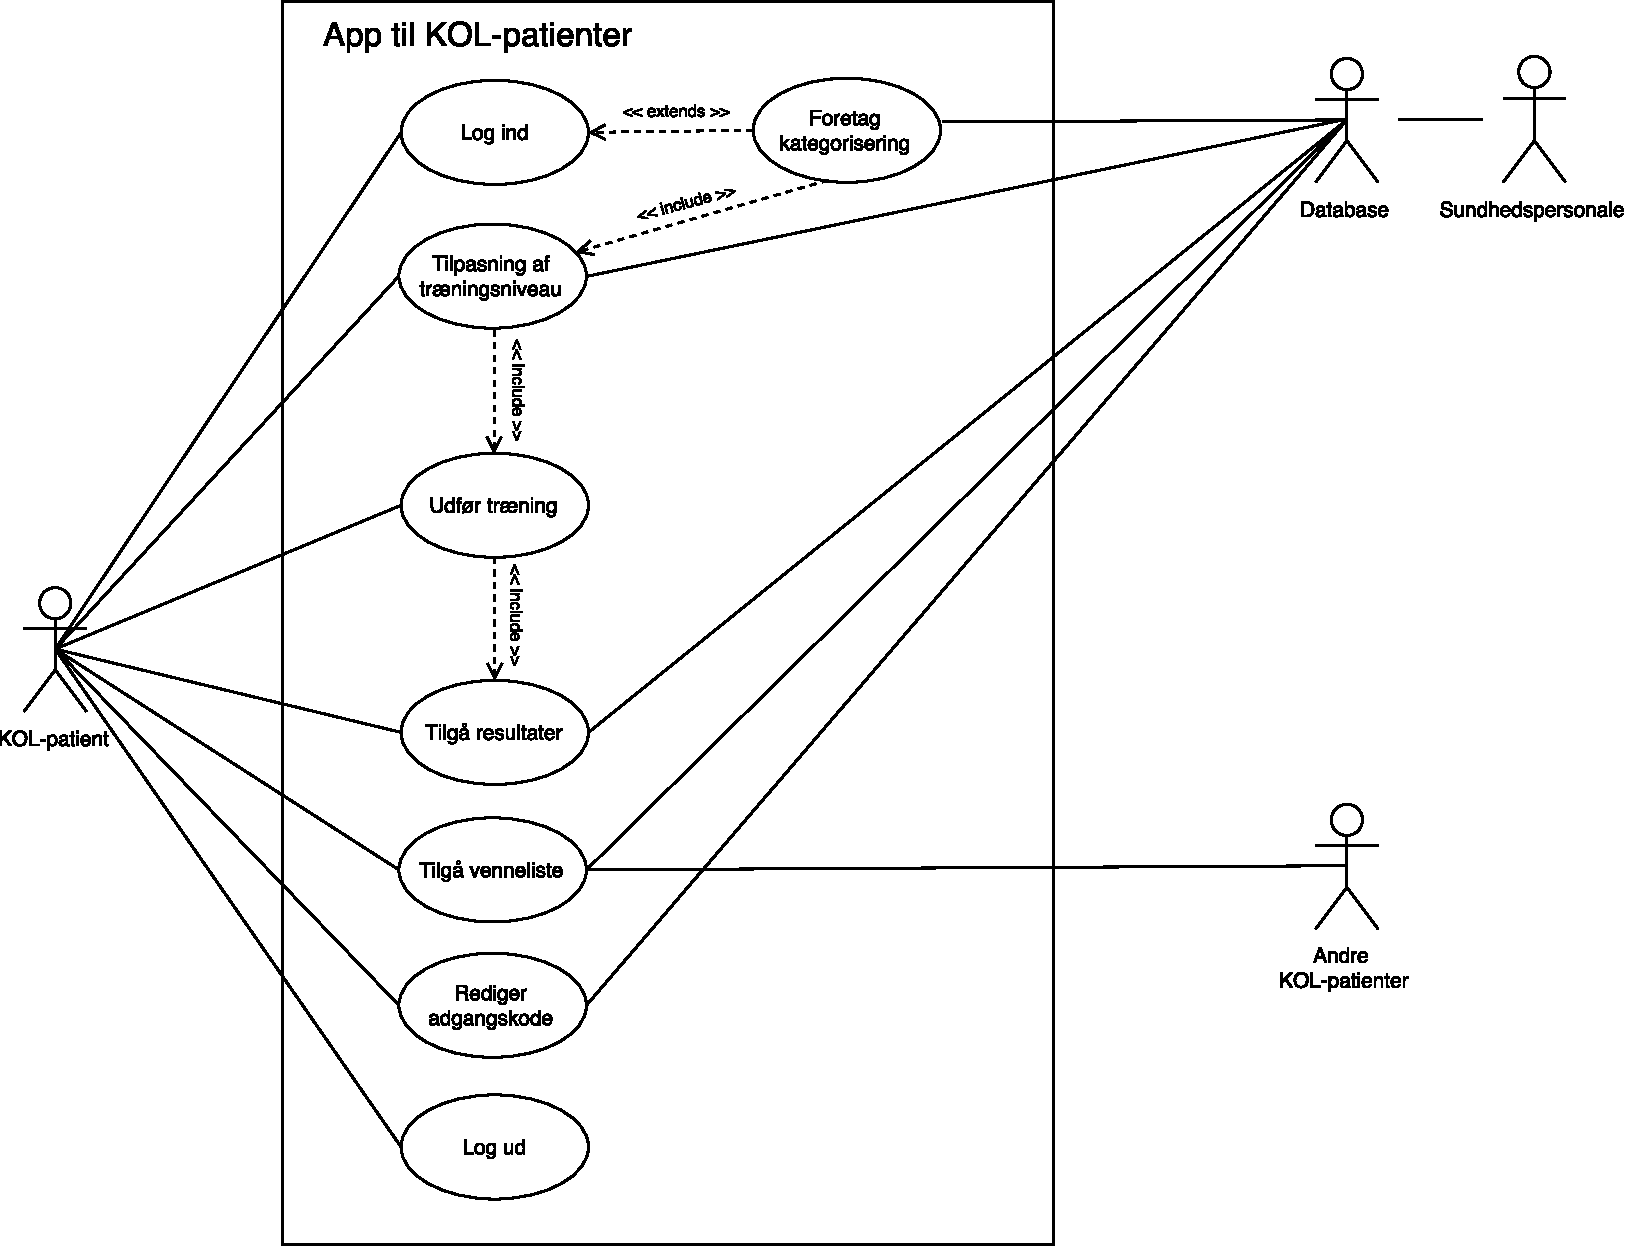
\includegraphics[width=0.9\textwidth]{figures/aktivitetsdiagram/Usecase}
\caption{Use case for app til KOL-patienter}
\label{fig:usecase}
\end{figure}

\noindent
Efter KOL-patienter er logget ind i app'en har de adgang til en hovedmenu, hvorfra brugere kan vælge at redigere brugeroplysninger, udføre træning, se resultater og venneliste. 

I \textit{Redigering af brugeroplysninger} kan brugere redigere deres adgangskode og kategorisering. Det skal være muligt for brugeren at ændre disse, da de ved registrering får en adgangskode udleveret. Dertil skal det være muligt at gøre deres adgangskode personligt. Derudover kan deres tilstand grundet KOL ændres, hvorfor kategoriseringen skal kunne redigeres. Hvis der foretages ændringer gemmes disse efterfølgende i databasen. 

\textit{Valg af træningsniveau} tilpasses individuelt ud fra \textit{Patientstatus}, der vurderes ud fra \textit{Kategorisering}, \textit{Daglig helbredstilstand} samt \textit{Evaluering af træning}.
Under \textit{Træning} kan eksterne enheder tilkobles systemet, således målinger kan opsamles. Efter udført træning samt evaluering gemmes patientens status, træningsresultater samt målinger i \textit{Resultater} og databasen. Ved en udført træning startes en nedtælling, som efter 24 timer sender en \textit{Notifikation} med henblik på at motivere brugeren til træning. Hvis brugeren benytter app'en førend de 24 timer er gået, nulstilles timeren.
Brugere kan tilgå samtlige resultater, som visualiseres i en kalender, ved grafisk udvikling samt belønninger. Sundhedspersonalet kan kun tilgå udviklingen af brugerens træning, mens brugeren via \textit{Venneliste} kan vælge at tilgå andres belønninger. Dette medvirker til, at brugere kan motivere hinanden til at udføre træning. Efter hver handling returneres brugeren til hovedmenuen.
%% Aktivitetsdiagram
\section{Funktionalitet}
I dette afsnit beskrives funktionaliteterne, der er udarbejdet ud fra systembeskrivelsen samt use case diagrammet. De enkelte funktionaliteter er opdelt efter registrering, log ind, redigering, kategorisering af KOL, daglig helbredstilstand, træning, resultater og sociale relationer. 





*** NOGET AF DETTE KAN BRUGES NEDENFOR! ****
Da app'en skal implementeres på en mobilenhed skal der være nogle sikkerhedsforanstaltninger i forhold til at beskytte KOL-patienters personfølsomme oplysninger. Sundhedsdatastyrelsen har udarbejdet vejledning om informationssikkerhed i sundhedsvæsnet, herunder mobilsikkerhed \cite{Sundhedsdatastyrelsen2016}.

Da information fra mobileenheder har større risiko for at blive misbrugt, da uvedkommende kan tilgå informationer via netadgang eller enheden. For at reducere risikoen for dette skal app'en tilgås via brugernavn og adgangskode før brug. Derudover registreres KOL-patienter i en database i et sikkert miljø af sundhedspersonalet. Derudover angives patienterne med medlemsID fremfor personnummer for, at gøre patienter uidentificerbare \cite{Sundhedsdatastyrelsen2016}. 

\subsection*{Registrering} \label{sec:registrering}
Inden KOL-patienter kan anvende app'en skal de registreres som brugere af systemet. Dette skal foregå i forbindelse med rehabiliteringsforløbet, hvor sundhedspersonale opretter patienterne i databasen. Patienterne får tilknyttet et medlemsID og en adgangskode. MedlemsID'et består af tal, eksempelvis \textit{01170301}, som er sammensat ud fra lokalisation, årstal og måned for påbegyndt rehabilieringsforløb samt nummerering af den enkelte KOL-patient.
Adgangskoden, der bliver udleveret af sundhedspersonalet, kan senere ændres i app'en, hvis en personlig adgangskode ønskes. 

Under registrering skal KOL-patienter ligeledes vælge et brugernavn, som gør dem identificerbare, således andre brugere kan følge dem. Brugernavn tilføjes til databasen, og KOL-patienter kan dermed vælge at logge ind på app'en ved brug af brugernavn eller  medlemsID samt adgangskode. 

I forbindelse med registrering skal sundhedspersonalet introducere KOL-patienter til brugen af app'en. Herunder skal de hjælpe KOL-patienterne med at kategorisere patientens sygdom før app'en anvendes til træning i hjemmet. Dette skal gøres i et forsøg på at skabe tryghed hos patienterne, da denne kategorisering har betydning for, hvilket træningsniveau patienten senere får foreslået af app'en. Der er desuden mulighed for at kunne få besvaret eventuelle tvivlsspørgsmål, der kan opstå første gang app'en anvendes. 



**** Denne adgangskode skal være på minimum seks karakterer, jf. \autoref{sec:sikkerhed}. DET SKAL NED ****



\subsection*{Log ind}
I systemet benyttes en log ind funktion til at beskytte og identificere den enkelte bruger. Brugeren vil her angive log ind information, der vil tillade adgang til information i form af private oplysninger og tidligere resultater, tilknyttet den givne bruger. Aktiviteterne for log ind funktion fremgår af \autoref{fig:logind}.    


\begin{figure} [H]
\centering
\textbf{Aktivitetsdiagram: Log ind}\par\medskip
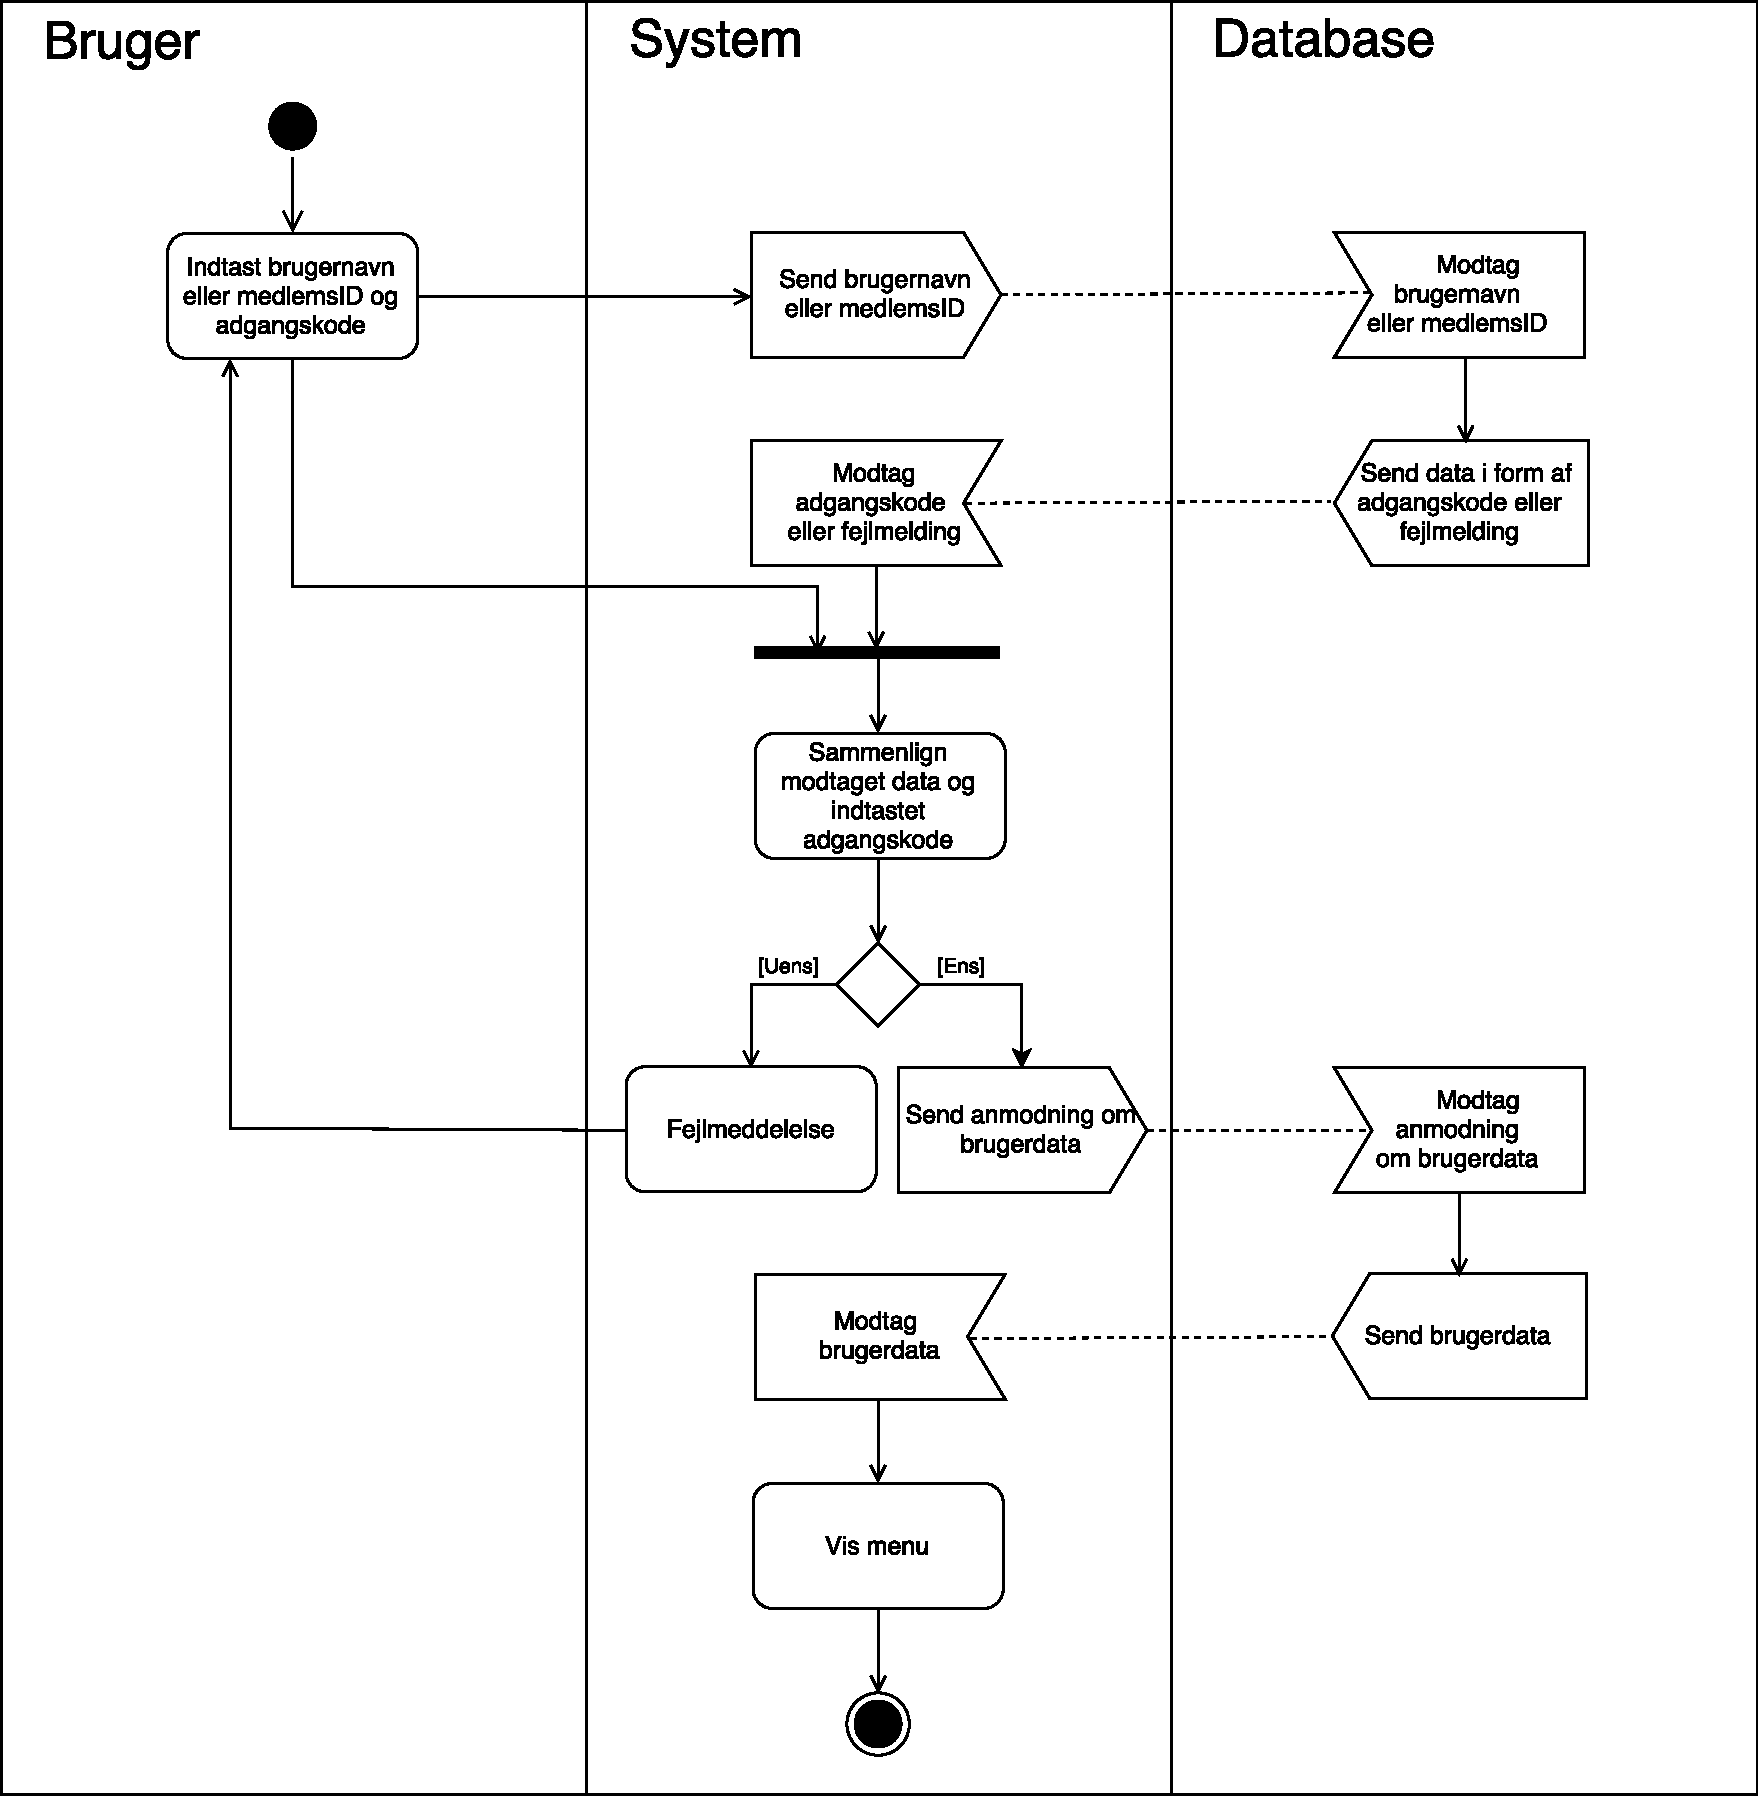
\includegraphics[width=0.9\textwidth]{figures/aktivitetsdiagram/Logind}
\caption{Aktivitetsdiagram for log ind}
\label{fig:logind}
\end{figure}


\noindent
Idet brugeren åbner app'en, vil en grænseflade for log ind vises. Hertil er det ikke muligt at gå videre gennem aktiviteterne, før brugeren har angivet log ind information, i form af medlemsID og en adgangskode. 
Såfremt at medlemsID'et findes, benyttes det efterfølgende i databasen til at identificere den korrekte adgangskode og returnere denne til systemet. Findes medlemsID'et ikke vil dette resultere i at systemet vil vise en fejlmeddelelse, og returnere til grænsefladen for log ind. 
Idet den korrekte adgangskode modtages af systemet, sammenlignes denne med angivet adgangskode. I tilfælde af at adgangskoderne ikke er identiske, vises en fejlmeddelelse og systemet returnere til grænsefladen for log ind. Er adgangskoderne identiske vil systemet hente alt brugerrelateret information fra databasen. I tilfælde af at data'en ikke modtages vises en fejlmeddelelse, ellers tjekkes om det er første gang brugeren logger ind på appen. 
Ved førstegangs log ind vil systemet udføre en aktivitet, hvorigennem systemet får angivet brugerens kategorisering af KOL. Efter angivelsen af kategoriseringen, eller ved efterfølgende log ind vil systemet gå direkte til at vise hovedmenuen.  
    

%Når KOL-patienten vil anvende app'en skal medlemsID eller brugernavn samt kodeord indtastes. Systemet sender det indtastede medlemsID eller brugernavn til databasen, som tilbagesender det tilhørende kodeord, hvis det findes i databasen. Findes de indtastede informationer ikke, sendes en fejlmeddelelse i form af 0. Systemet sammenligner herefter brugerens indtastede adgangskode med adgangskoden fra databasen. Er de to værdier ens, har brugeren indtastet de korrekte informationer, hvortil brugerdata hentes fra databasen og hovedmenuen vises. Brugerdata omfatter brugerens informationer og tidligere resultater. Er de to værdier ikke ens, tilbagesender systemet en fejlmeddelelse, og brugeren får derefter mulighed for at indtaste log ind informationen igen. 
\subsubsection*{Kategorisering} \label{sec:kategorisering}
Første gang KOL-patienter logger ind i app'en, skal de foretage en individuel kategorisering. Dette er nødvendigt for at sikre, at brugeren får anbefalet et træningsniveau, som passer til deres helbred.
Kategoriseringen inddeler brugerne i A, B, C eller D, som beskrevet i \autoref{sec:klassifikation}. Af \autoref{fig:Kate} ses aktivitetsdiagrammet for kategoriseringen.

\begin{figure} [H]
\centering
\textbf{Aktivitetsdiagram: Kategorisering af KOL-patienter}\par\medskip
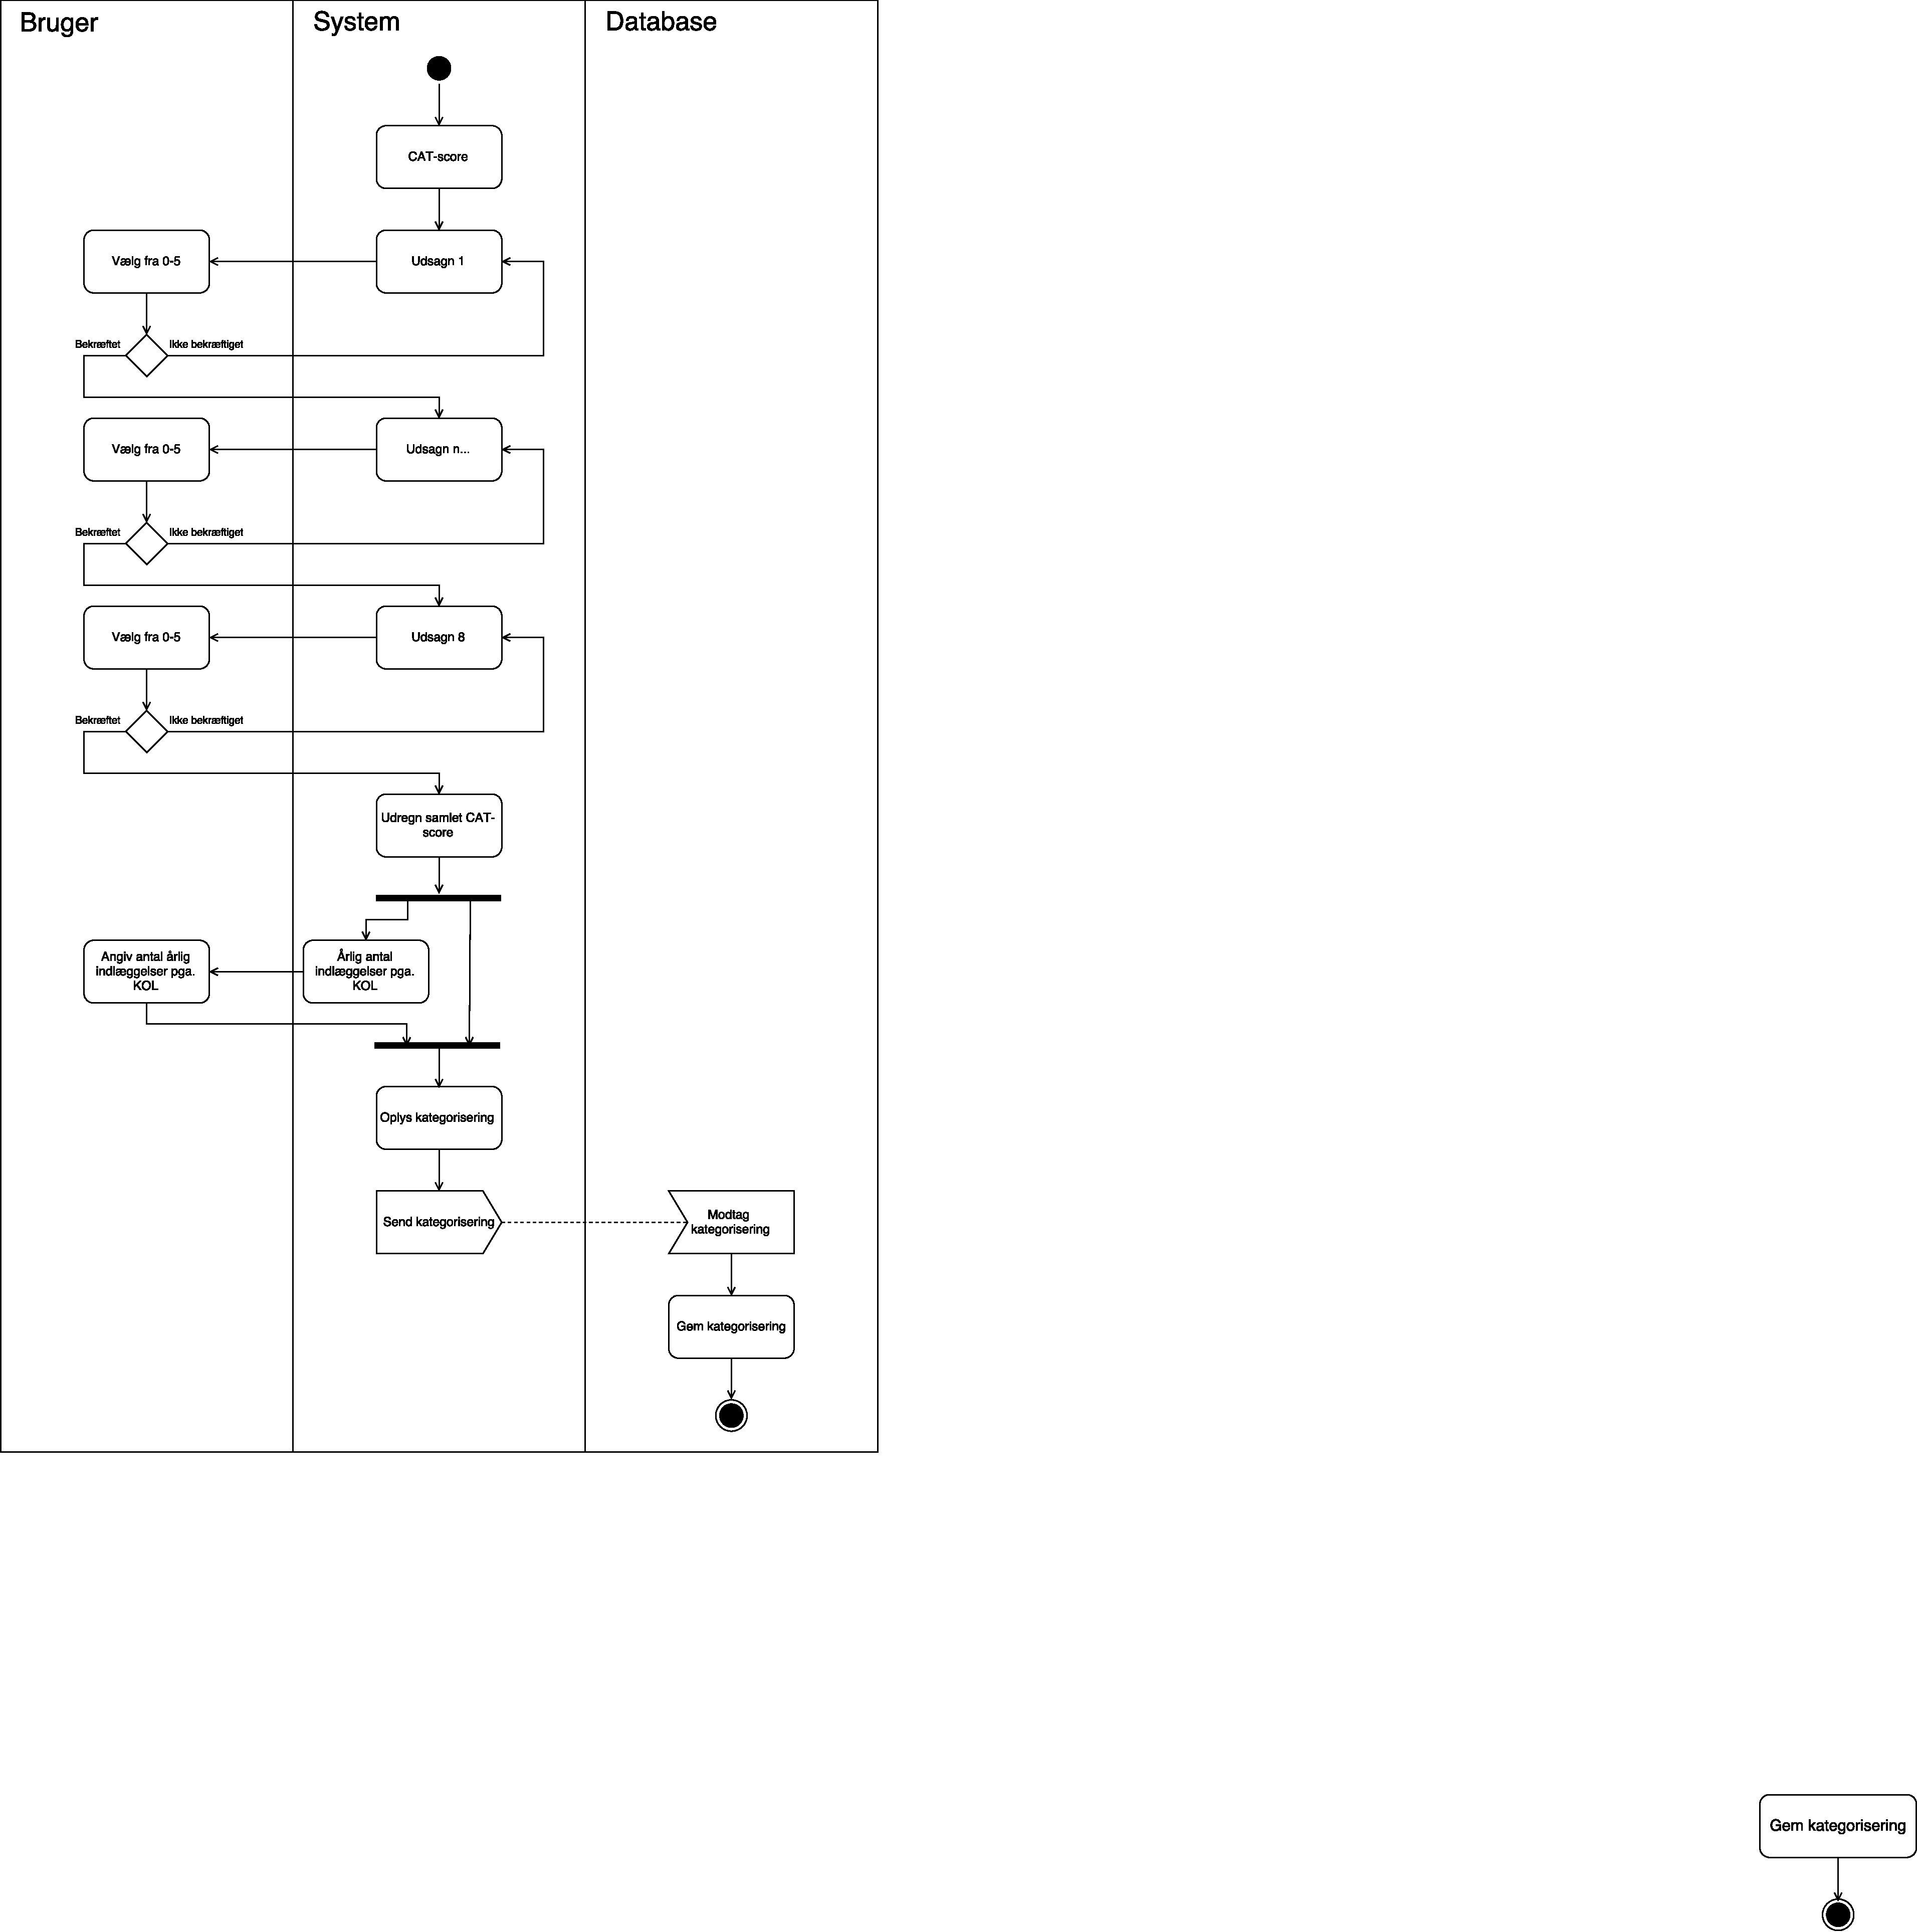
\includegraphics[width=1\textwidth]{figures/aktivitetsdiagram/Kategorisering}
\caption{Aktivitetsdiagram for kategorisering af KOL-patienter.}
\label{fig:Kate}
\end{figure}

\noindent
Systemet starter med at vise en grænseflade for hver af de otte udsagn, der udgør CAT-scoren, jf. \autoref{fig:CAT}. Til hvert af udsagnene angiver brugeren en score passende til deres sygdomstilstand, hvor systemet ud fra de individuelle score beregner en samlet CAT-score. 
Dernæst vises grænsefladen for årlig antal indlæggelser forårsaget af KOL, hvor brugeren skal angive antal indlæggelser årligt. Ud fra den samlede CAT-score og antal indlæggelser, beregner systemet brugerens kategorisering af KOL. Efterfølgende viser systemet brugerens kategorisering som  A, B, C eller D.
Kategoriseringen sendes og gemmes i databasen.  
%\subsection*{Daglig helbredstilstand}
Førend en træning påbegyndes skal brugerens daglige helbredstilstand angives. Dette er for at sikre, at træningen tilpasses den individuelle bruger samt imødekomme dag til dag variationer. Af \autoref{fig:helbredstilstand} fremgår aktivitetsdiagrammet for angivelse af den daglige helbredstilstand. 

\begin{figure} [H]
\centering
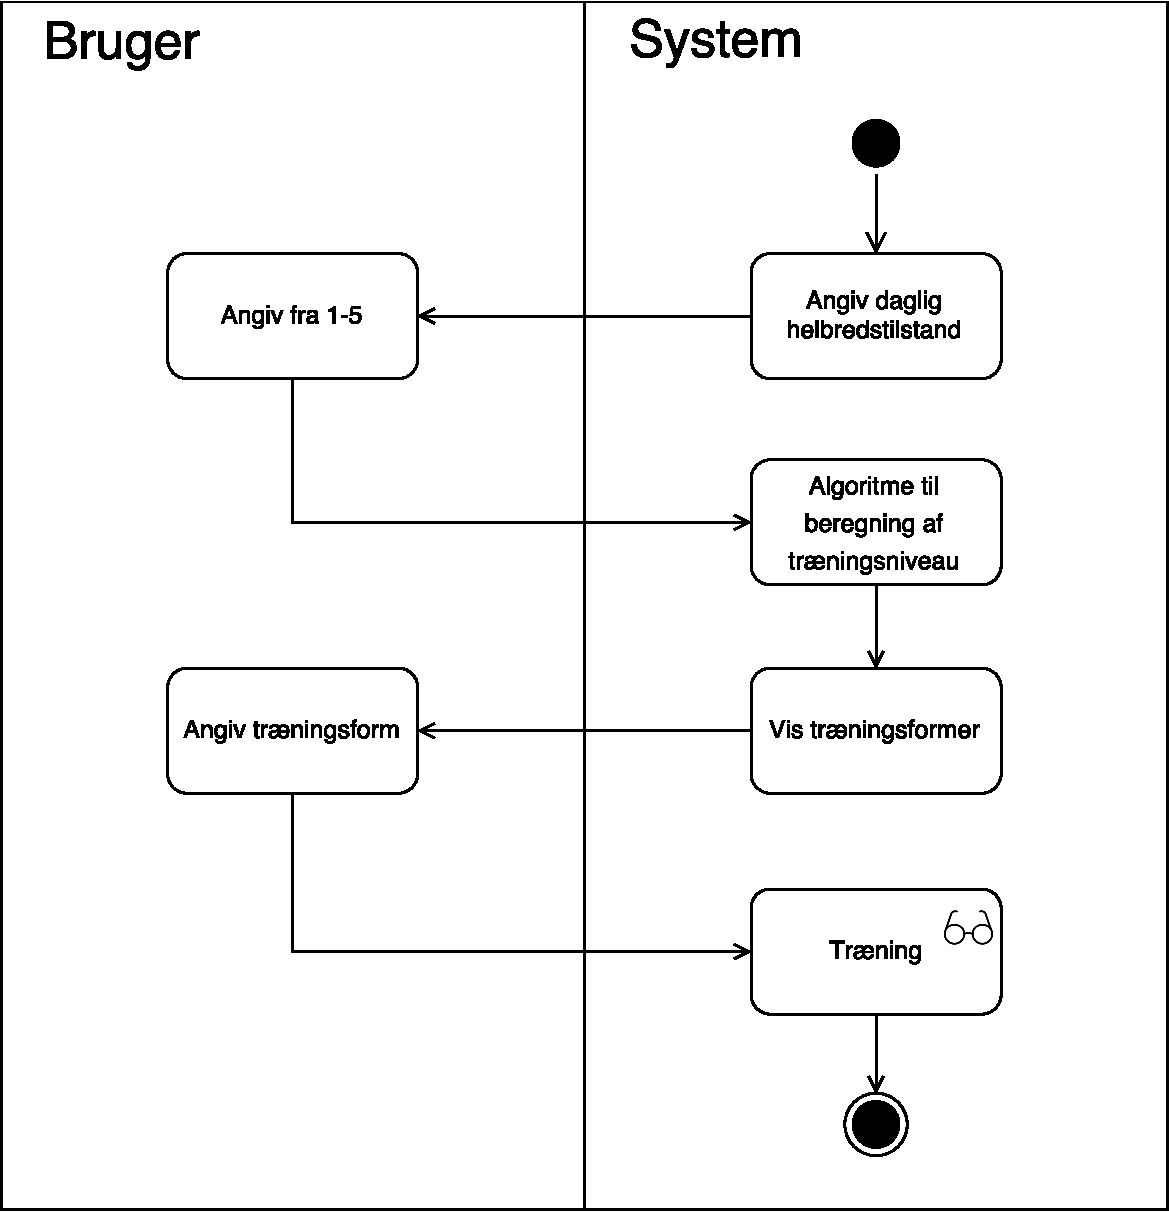
\includegraphics[width=0.9\textwidth]{figures/aktivitetsdiagram/Helbredstilstand}
\caption{Aktivitetsdiagram for daglig helbredstilstand. Træning er yderligere beskrevet af \autoref{fig:traening}.}
\label{fig:helbredstilstand}
\end{figure}

\noindent
Den daglige helbredtilstand angives ved hjælp af en skala fra 1, svarende til en dårlig helbredstilstand, til 5, svarende til en god helbredstilstand. Ud fra den daglige helbredstilstand, kategoriseringen af KOL samt evaluering fra førhenværende træning, passende til den angivede helbredstilstand, vælges et træningsniveau passende til brugerens nuværende helbred. Dertil foreslås brugeren forskellige træningsformer, herunder konditions-, styrketræning samt vejrtrækningsøvelser. Den ønskede træningsform vælges, hvortil træningen kan udføres. Træningen er yderligere beskrevet af \autoref{fig:traening}. 


*** Beslutningstræ! ***
\subsection*{Træning} \label{sec:traening}
Brugeren har mulighed for at fortage træninger baseret på forskellige træningsformer og træningstyper. Derudover skal træningen kunne tilpasses individuelt under hver enkelt træningssession, samt tilkolbe yderligere måleenheder for at opnå en mere vejledende og fyldestgørende træning.  
Aktivitetsdiagrammet over træningen fremgår af \autoref{fig:traening}. 

\begin{figure} [H]
\centering
\textbf{Aktivitetsdiagram: Træning}\par\medskip
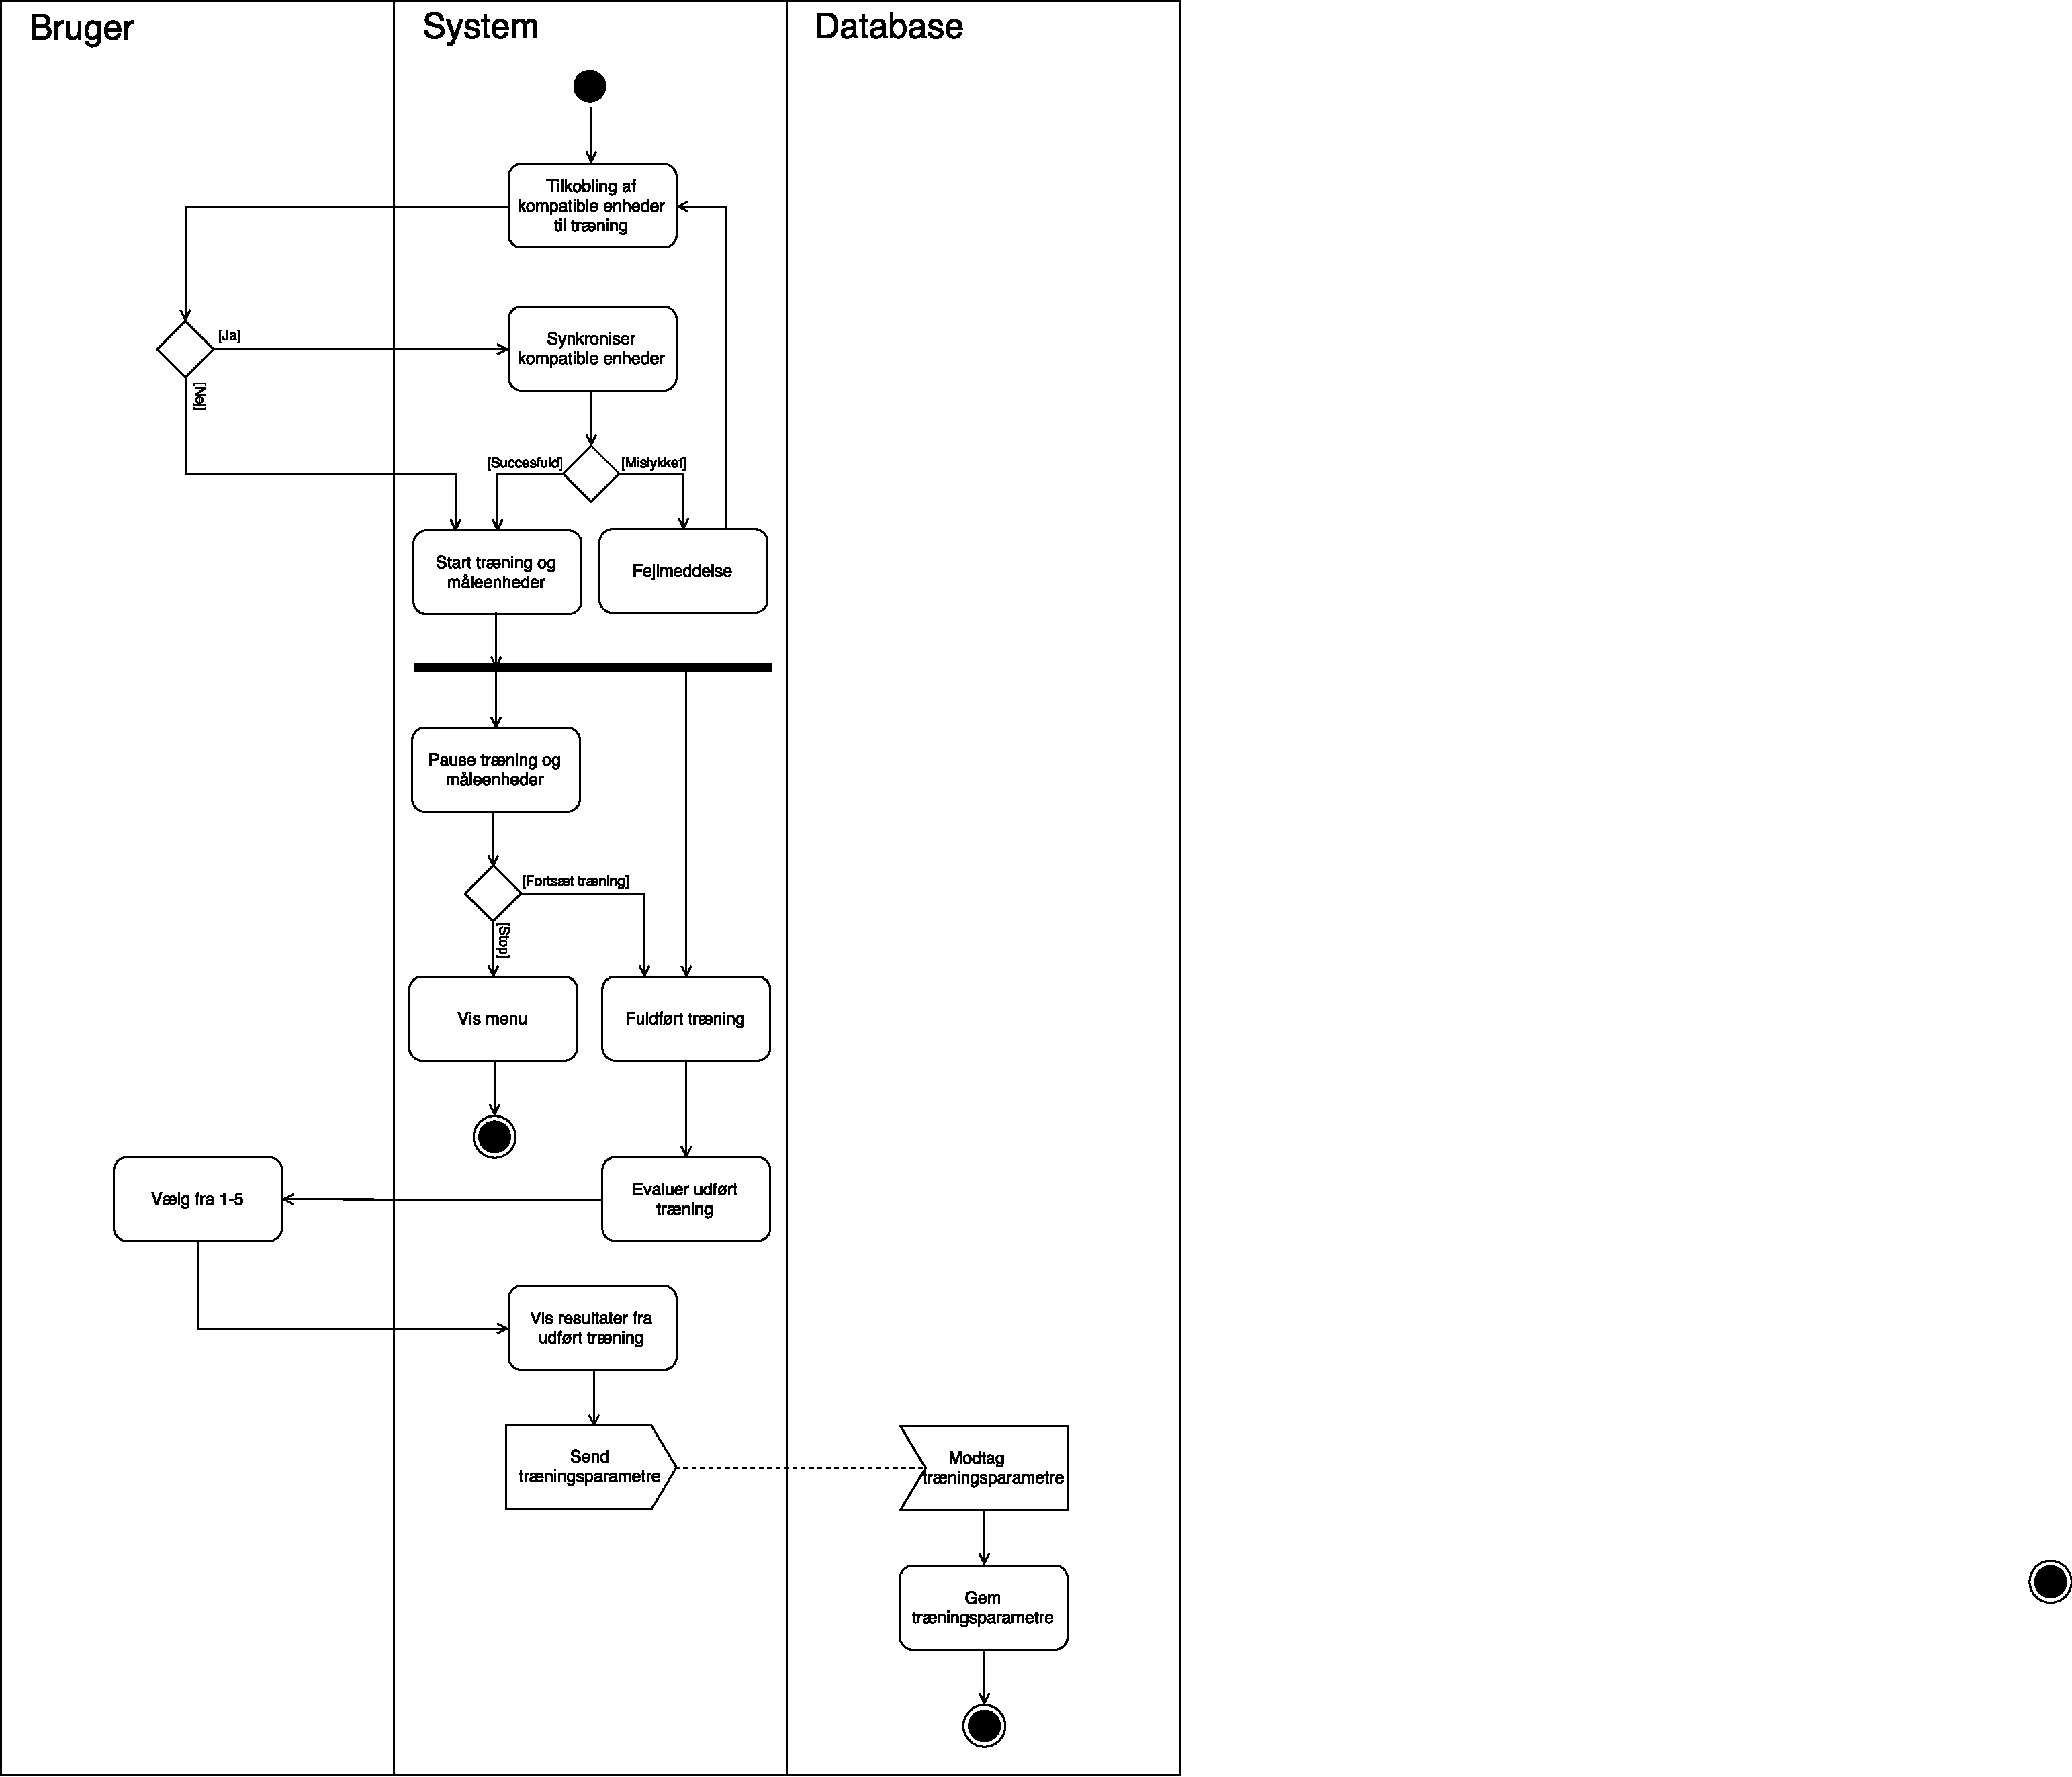
\includegraphics[width=0.8\textwidth]{figures/aktivitetsdiagram/Traening}
\caption{Aktivitetsdiagram over træning.}
\label{fig:traening}
\end{figure}

\noindent
Før selve træningen påbegyndes, skal brugeren angive den ønskede træningsform, herunder konditions-, styrketræning eller vejrtrækningsøvelser. Ud fra den valgte træningsform skal brugeren angive træningstype, eksempelvis kan der i forlængelse af konditionstræning vælges gå, løbe eller cykle. 
Efterfølgende tilpasses træningsniveauet til den enkelte bruger, og er beskrevet af et særskilt aktivitetsdiagram i \autoref{fig:traeningsniveau}.
Systemet vil efterfølgende undersøge om der er kompatible måleenheder til rådighed, og tilkoble dem til træningen før den påbegyndes af brugeren. 
Under træningen vil systemet kontinuert vise træningen og målinger der fortages. Brugeren kan til hver en tid vælge at afslutte træningen, dog skal denne handlingen bekræftes i tilfælde af at brugeren ved fejl angiver at træningen skal stoppes. 
Systemet stopper dermed træningen og afventer en evalueringen som skal angives af brugeren. 
Efter at træningssættet er evalueret sender systemet informationen relateret til træningssessionen til databasen, hvor det gemmes.  

\subsection*{Tilpasning af træningsniveau} \label{sec:traeningsniveau}
Tilpasning af træningsniveau er en funktion der skal varetage træningen for brugeren, ved at anbefale et træningsniveau ud fra brugeres kategorisering, dag til dag variationer og tidligere evalueringer af træninger. Aktivitetsdiagrammet over valg af træningsniveau fremgår af \autoref{fig:traening}.
 
\begin{figure} [H]
\centering
\textbf{Aktivitetsdiagram: Valg af træningsniveau}\par\medskip
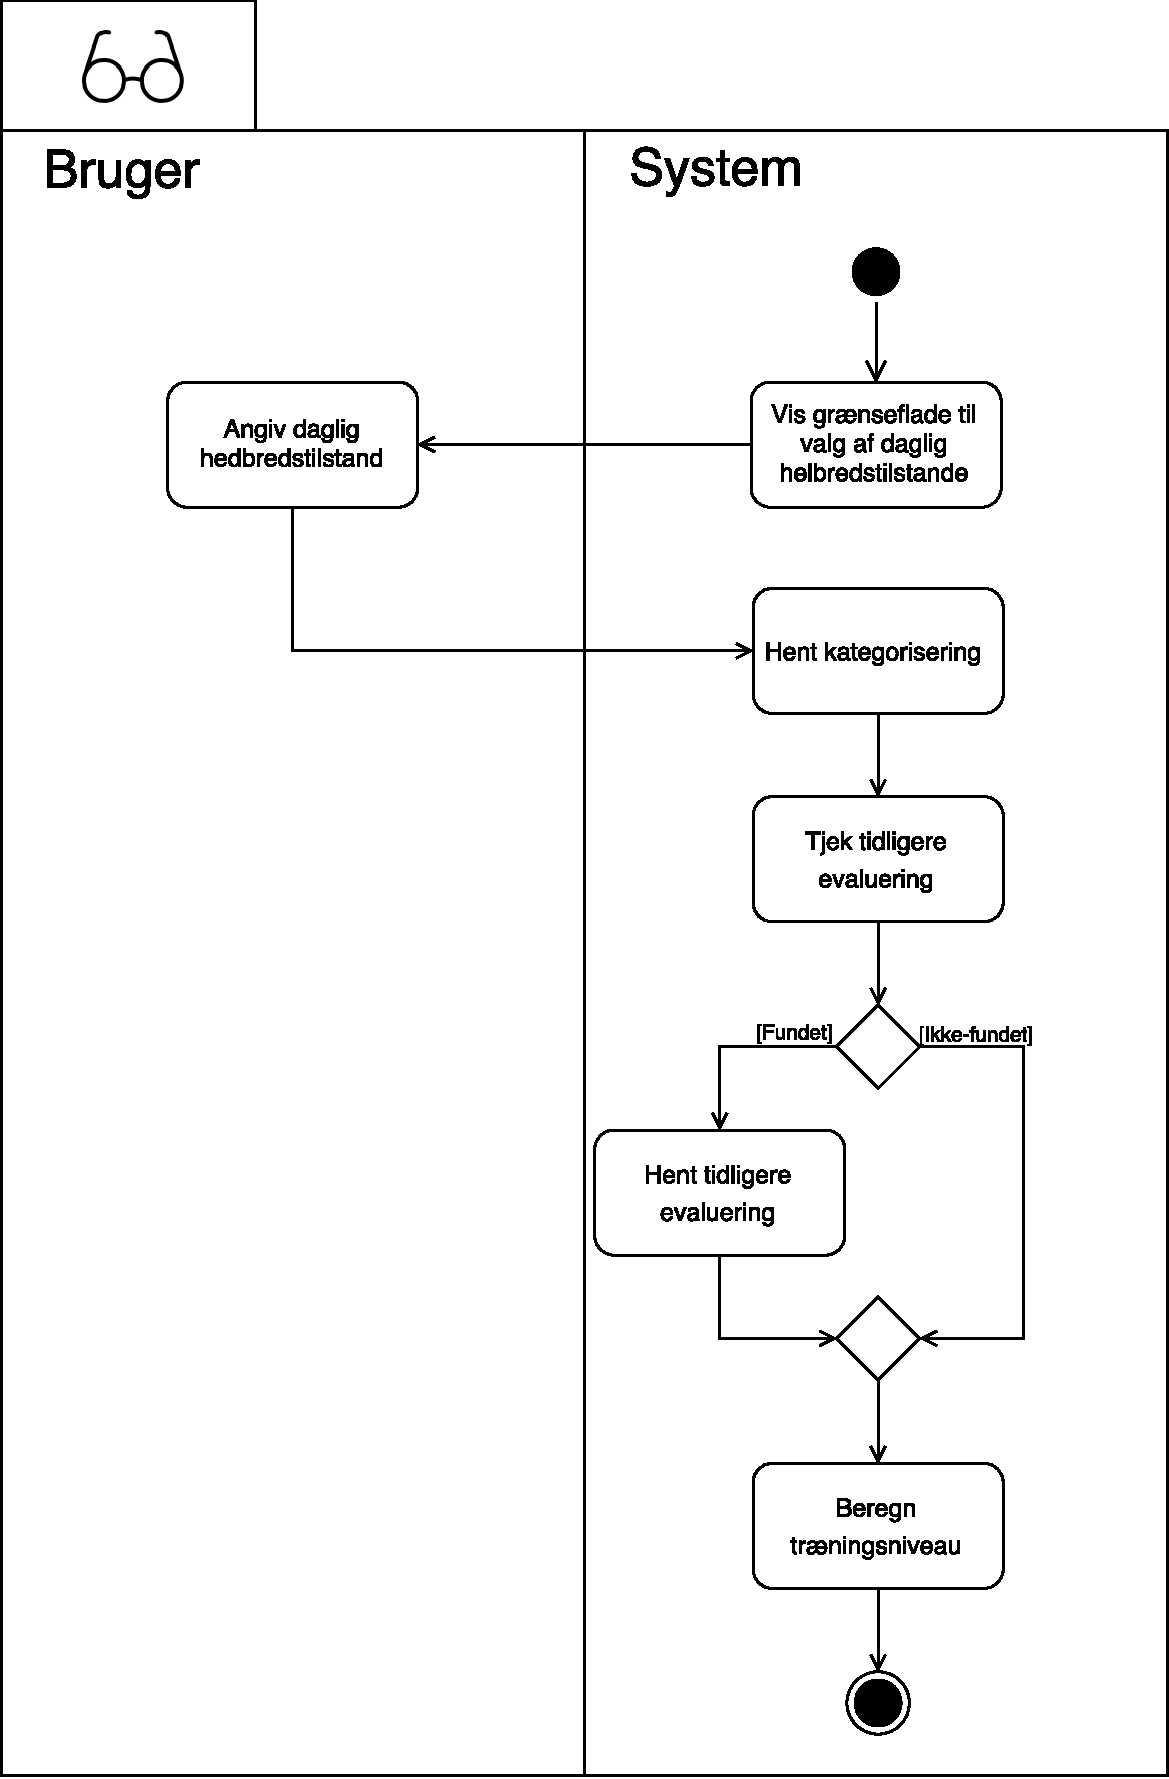
\includegraphics[width=0.8\textwidth]{figures/aktivitetsdiagram/Tilpasningaftraeningsniveau}
\caption{Aktivitetsdiagram over valg af træningsniveau.}
\label{fig:traeningsniveau}
\end{figure}

\noindent
Valg af træningsniveau ses som en aktivitet i aktivitetsdiagrammet for træning i \autoref{fig:traening}. For at systemet kan tilpasse træningsniveauet, vil brugeren skulle angive sin helbredstilstand før den givne træning. Yderligere beregnes træningsniveauet af brugers kategorisering, som blev defineret første gang brugeren loggede ind på app'en, og på tidligere evalueringer, såfremt tidligere evalueringer er fortaget.


Tilpasningen af træningsniveauet kan også visualiseres som en simpel beslutningstabel, der ses af \autoref{tab:beslutningstabel}. Tabellen beskriver hvordan en algoritme, ville regulere i træningsniveauet således det er passende til den enkelte bruger.  

\subsubsection*{Algoritme til tilpasning af træningsniveau}
Algoritmen til valg af træningsniveau er illustreret som en simpel beslutningstabel, der viser, hvilke parameter, som ligger til grund for valg af træningsniveau til den enkelte bruger. Af \autoref{tab:beslutningstabel} ses beslutningstabellen for valg af træningsniveau.

\begin{table}[H]
\centering
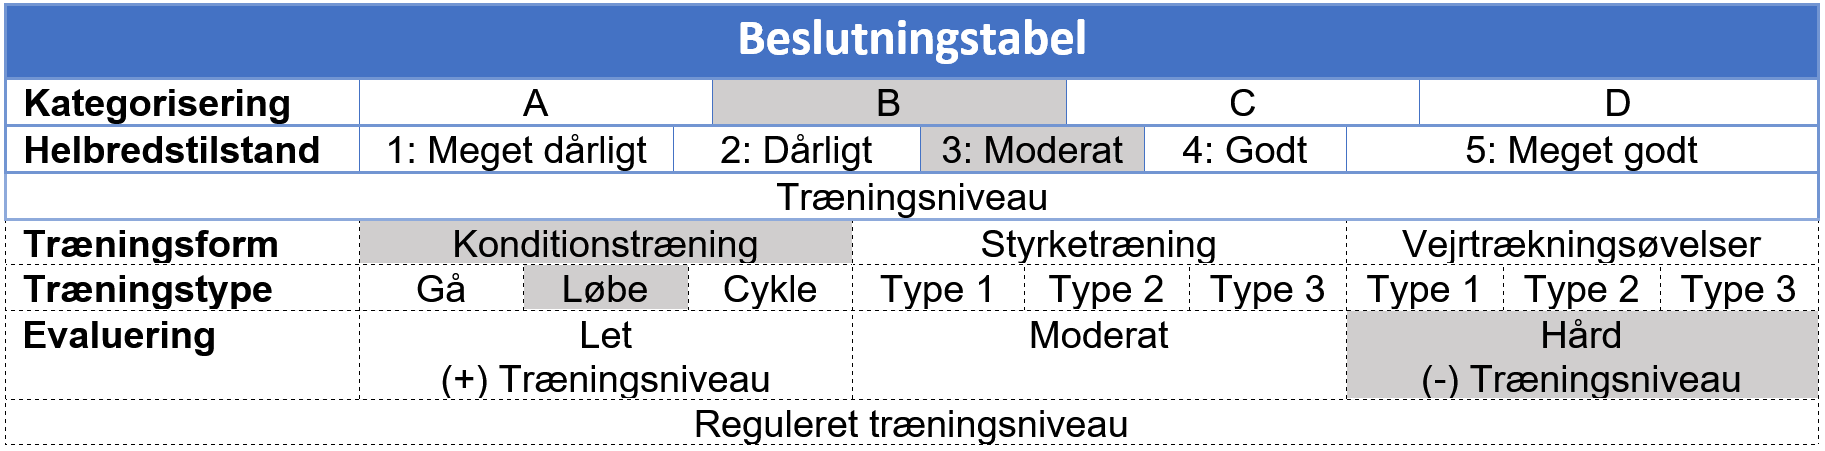
\includegraphics[width=1\textwidth]{figures/aktivitetsdiagram/beslutningstabel}
\caption{Beslutningstabel for træningsniveau. Kategorisering, daglig helbredstilsand samt eventuel evaluering medregnes til at bestemme træningsniveau til den enkelte træning. Af dette eksempel er brugeren kategoriseret B med en helbredstilstand, der er angivet som moderat. Dertil har brugeren valgt løb under konditionstræning. Tidligere har brugeren haft samme daglig helbredstilstand samt træning, og evalueret denne træning som værende hård. Dette muliggøre en regulering af træningsniveauet, hvorfor niveauet i dette tilfælde sænkes.}
\label{tab:beslutningstabel}
\end{table} 

\noindent
Af \autoref{tab:beslutningstabel} fremgår en simpel beslutningstabel for, hvorledes et træningssæt tilpasses den enkelte bruger. Beslutningstabellen tager udgangspunkt i brugerens kategorisering, daglig helbredstilstand samt en eventuel evaluering. Brugeren er i dette tilfælde kategoriseret til B. Helbredstilstanden angives førend en træning påbegyndes, for således at tilpasse niveauet til den pågældende dag. Helbredstilstanden angives efter \textit{1: Meget dårligt}, \textit{2: Dåligt}, \textit{3: Moderat}, \textit{4: Godt} eller \textit{5: Meget godt}, hvortil brugerens helbredstilstand her angives som moderat
Træningsniveauet vurderes dermed ud fra brugerens kategorisering samt helbredstilstand. 
For at have mulighed for at kunne regulere træningssættet yderligere, medregnes den forhenværende evaluering, der er forbundet med samme helbredstilstand, træningsform og type. I dette tilfælde har brugeren før haft samme helbredstilstand, træningsform samt type og dertil evalueret denne træning til værende hård. Algoritmen regulerer hertil træningsniveauet for denne træning ned, for således at give brugeren en bedre træningsoplevelse. 

\subsection*{Resultater}
Fra app'ens hovedmenu kan brugeren tilgå sine resultater, der visualiseres grafisk og ved virtuelle belønninger.
Aktivitetsdiagrammet over resultater fremgår af \autoref{fig:resultater}.

\begin{figure} [H]
\centering
\textbf{Aktivitetsdiagram: Resultater}\par\medskip
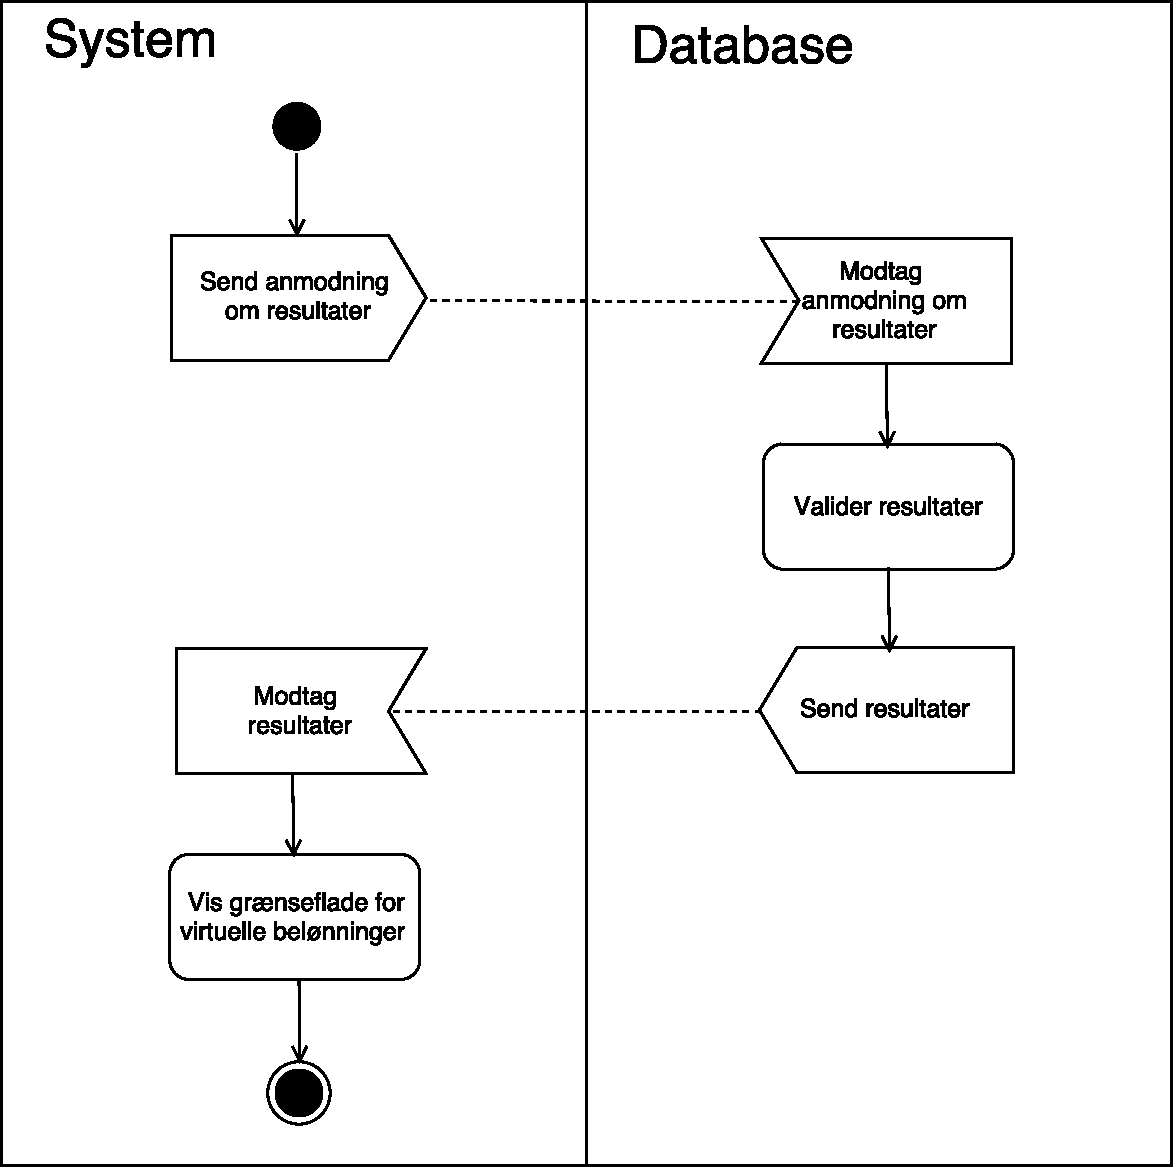
\includegraphics[width=0.95\textwidth]{figures/aktivitetsdiagram/Resultater}
\caption{Aktivitetsdiagram over resultater.}
\label{fig:resultater}
\end{figure}

\noindent
Under resultater er det muligt for brugeren at se sin ugentlige træning samt virtuelle belønninger. Idet brugeren tilgår resultater fra hovedmenuen, hentes resultater, der vises som en grafisk udvikling, fra databasen. Brugeren har fra grænsefladen for grafisk udvikling mulighed for at tilgå sine belønninger. Ønskes dette, hentes brugerens belønninger fra databasen, hvorefter de visualiseres i grænsefladen for belønninger. Belønningerne varierer afhængig af træningsform, og der kan opnås forskellige belønninger inden for forskellige kategorier. 

%Et eksempel på fordeling af belønninger i forskellige kategorier fremgår af \autoref{tab:beloenninger}.
%
%\begin{table} [H]
%\centering
%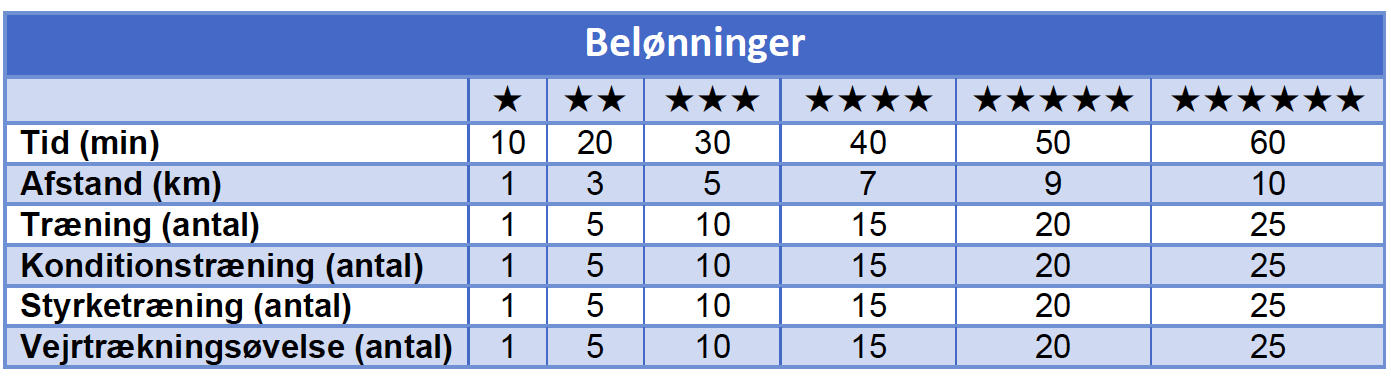
\includegraphics[width=1\textwidth]{figures/aktivitetsdiagram/beloenninger}
%\caption{Eksempel på belønninger opnået ved træning inden for forskellige kategorier.}
%\label{tab:beloenninger}
%\end{table}
%
%\noindent
%Ud fra \autoref{tab:beloenninger} fremgår et eksempel på fordeling af virtuelle belønninger, der er opdelt efter afstand, tid og antallet af gennemførte træninger. 
\subsection{Social relationer} 
For at motivere KOL-patienter til en regelmæssig træning, vælges at integrere muligheden for sociale relationer i app'en. Dette muliggøre, at brugere kan følge hinanden og derved se, hvilke belønninger andre brugere har opnået. Hertil skal det være muligt for brugeren at tilføje og fjerne venner fra deres venneliste. 
Af \autoref{fig:venner} fremgår et aktivitetsdiagram for sociale relationer. 

\begin{figure} [H]
\centering
\includegraphics[width=0.65\textwidth]{figures/aktivitetsdiagram/venner}
\caption{Aktivitetsdiagram for sociale relationer.}
\label{fig:venner}
\end{figure}

\noindent
Vennelisten viser en oversigt over andre brugere, som den individuelle bruger vælger at følge. Heraf skal det være muligt for den individuelle bruger at tilgå information fra disse andre brugere. Denne information begrænses til at vise vundet belønninger for de andre brugere, da den resterende information anses som værende personlig til den enkelte bruger. 
Fra vennelisten skal den individuelle bruger have mulighed for at fjerne brugere fra vennelisten eller tilføje andre brugere, hvortil disse funktioner uddybes af henholdsvis \autoref{fig:venner} og \autoref{fig:tilfoejven}.  
Ønskes det at fjerne en bruger fra vennelisten, sendes informationer om den valgte bruger til databasen, hvorved vennerelationen slettes. Derefter returneres en bekræftigelse, der viser, at den valgte bruger er fjernet fra vennelisten. 

\begin{figure} [H]
\centering
\includegraphics[width=0.65\textwidth]{figures/aktivitetsdiagram/foelgnyven}
\caption{Aktivitetsdiagram for tilføjelse af venner til vennelisten.}
\label{fig:tilfoejven}
\end{figure}

Ved tilføjelse af nye bruger indtastes brugernavnet eller medlemsID'et på den givne bruger. Brugernavnet eller medlemsID'et sendes til databasen, der returnerer et brugernavn, medlemsID, vennerelation eller fejlmelding til systemet. Hvis der allerede er en relation mellem de to brugere eller, at brugerinformationen ikke eksisterer i databasen, forekommer en fejlmelding, hvortil et andet brugernavn eller medlemsID kan indtastes på ny. 
Såfremt, at der ikke forekommer en fejlmelding vises den søgte bruger, hvortil det er muligt at følge vedkommende. 
Vælges dette, sendes en anmodning til databasen som opretter en vennerelation mellem de to brugere. Efterfølgende returneres en bekræftelse om vennerelationen til systemet.
\subsection{Redigering af brugeroplysninger}
Brugeren skal ud fra app'ens hovedmenu have mulighed for at redigere private samt sygdomsspecifikke oplysninger. Dette er med henblik på, at brugeren selv skal kunne ændre sin adgangskode samt sin kategorisering, hvis deres helbred forværres. Af \autoref{fig:Redigerbrugeroplysninger} er aktivitetsdiagrammet for redigering af brugeroplysninger illustreret. 

\begin{figure} [H]
\centering
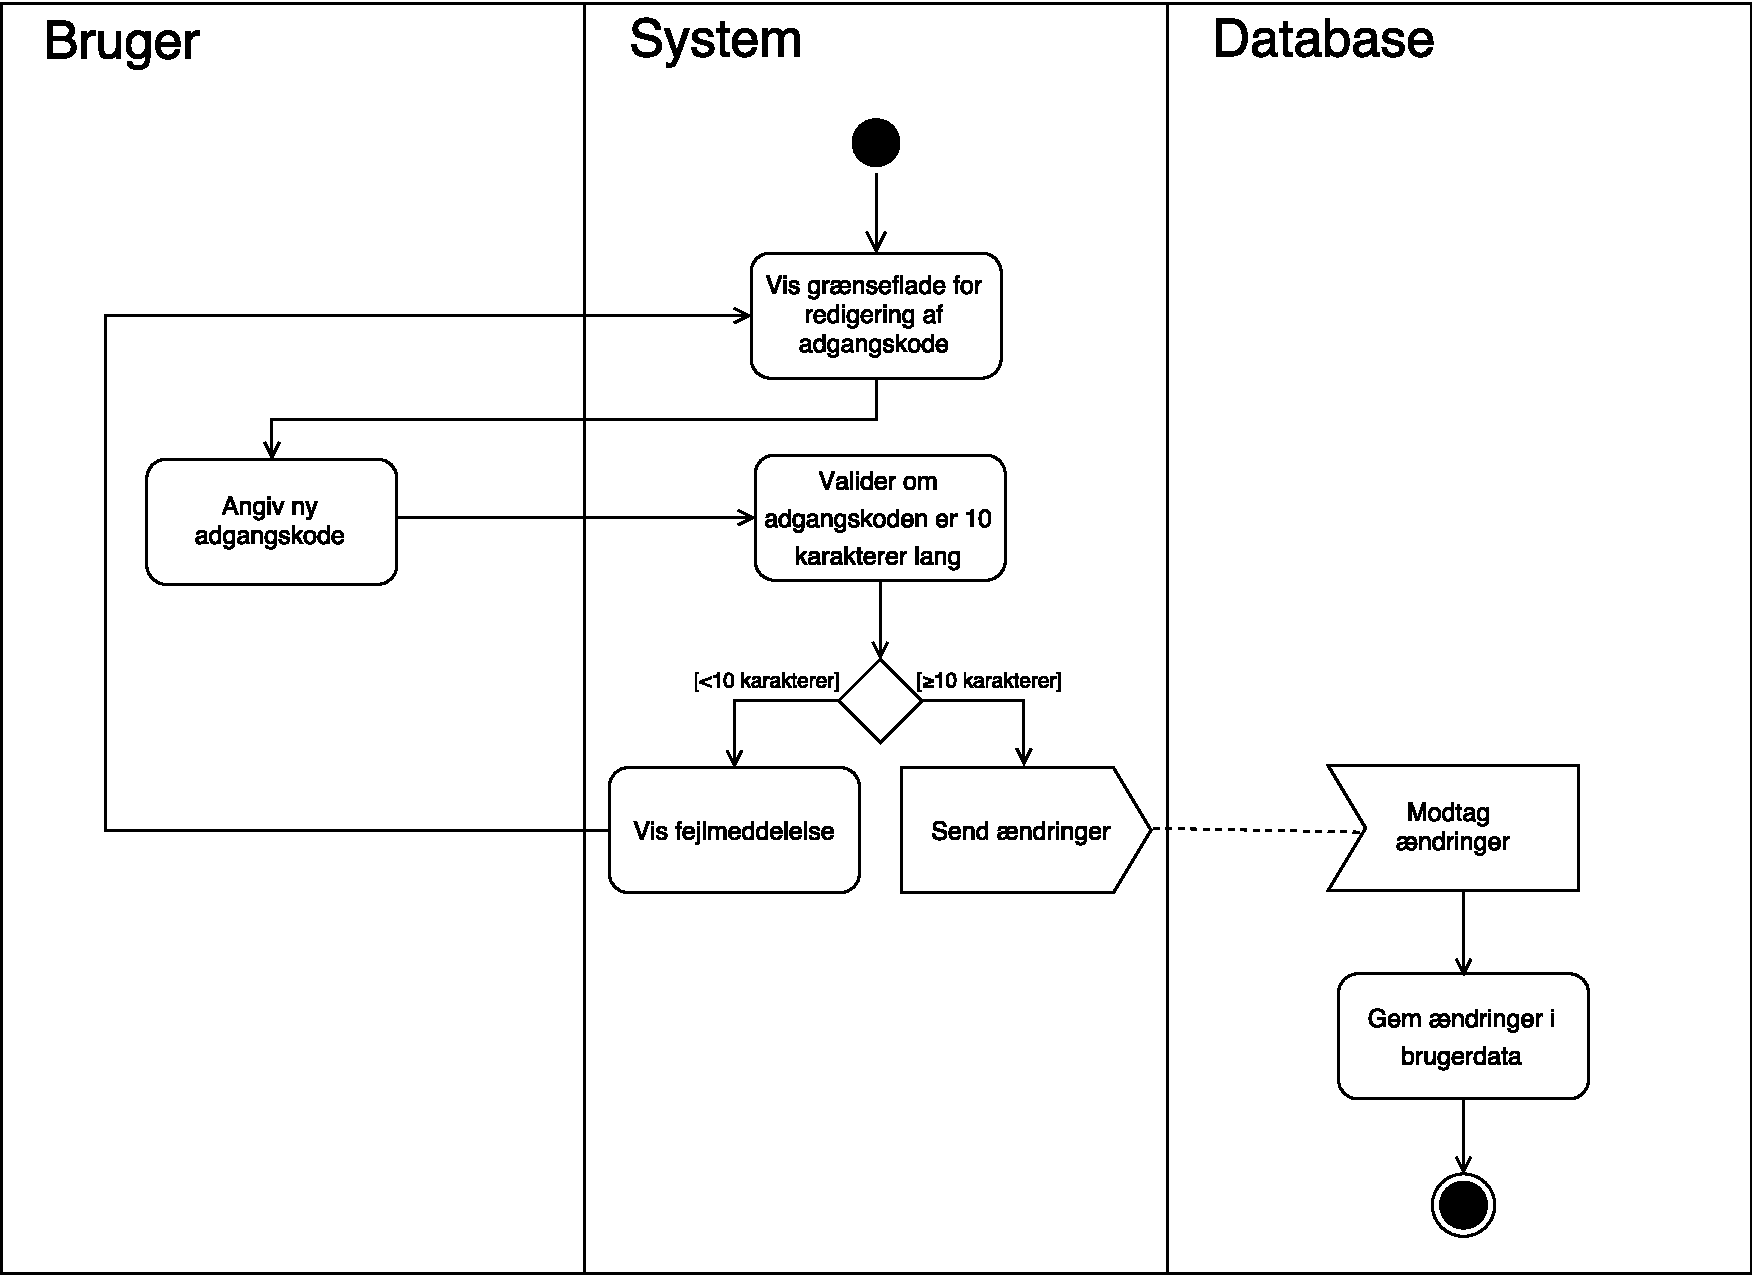
\includegraphics[width=0.9\textwidth]{figures/aktivitetsdiagram/Redigerbrugeroplysninger}
\caption{Aktivitetsdiagram for redigering af brugeroplysninger.}
\label{fig:Redigerbrugeroplysninger}
\end{figure}

Det skal både være muligt at ændre sin adgangskode samt kategoriseringen, som blev defineret første gang brugeren loggede ind på app'en. Da brugeren ved registrering får tildelt en tilfældig adgangskode, jf. \autoref{sec:registrering}, skal det være muligt at ændre denne til en personlig adgangskode. For at kunne foretage en ændring af adgangskoden, skal den nye adgangskode som minimum være seks karakterer lang. Hvis dette ikke opfyldes sendes en fejlmeddelse tilbage til brugeren, hvortil en ny adgangskode skal indtastes. 
I tilfælde af, at brugerens tilstand ændres er det ligeledes muligt at redigere denne. I \autoref{sec:kategorisering} beskrives aktivtetsdiagrammet for kategoriseringen af KOL yderligere. 
Ved korrekt redigering af brugeroplysninger sendes ændringerne til databasen, hvorefter de gemmes.
\subsection*{Log ud}
I forlængelse af log ind funktionen, er det også en log ud funktion. Denne funktion tillader brugeren at logge sig ud af systemet, således at brugeren ikke forbliver logget ind, og tillader yderligere andre brugere at logge ind fra samme app.
Aktiviteterne for log ind funktion fremgår af \autoref{fig:logind}.

\begin{figure} [H]
\centering
\textbf{Aktivitetsdiagram: Log ud}\par\medskip
\includegraphics[width=0.9\textwidth]{figures/aktivitetsdiagram/Logud}
\caption{Aktivitetsdiagram over log ud, hvor aktiviteter forekommer hos brugen, systemet eller databasen.}
\label{fig:logud}
\end{figure}

Brugeren har fra hovedmenuen, muligheden for at logge ud af systemet. Vælger brugen dette, vil grænsefladen for log ud vises. 
Brugeren skal efterfølgende bekræfte at de ønsker at logge ud, før at systemet systemt gennemføre handlingen og vis grænsefladen for log ind. Brugeren kan dog også vælge at fortryde log ud handlingen, i tilfælde af at bruger ved fejl valgte log ud, hvor systemet vil returnere til hovedmenuen.  
\subsection*{Analyseklasser}
Inden analyseklasserne udarbejdes, foretages en analyse ud fra systembeskrivelsen, use case og funktionaliteter til at identificere substantiver og verber. Dette gøres for at sikre, at alle funktionaliteter indgår i klassediagrammet. Substantiver og verber fremgår af \autoref{tab:subverb}.

\begin{table}[H]
\centering
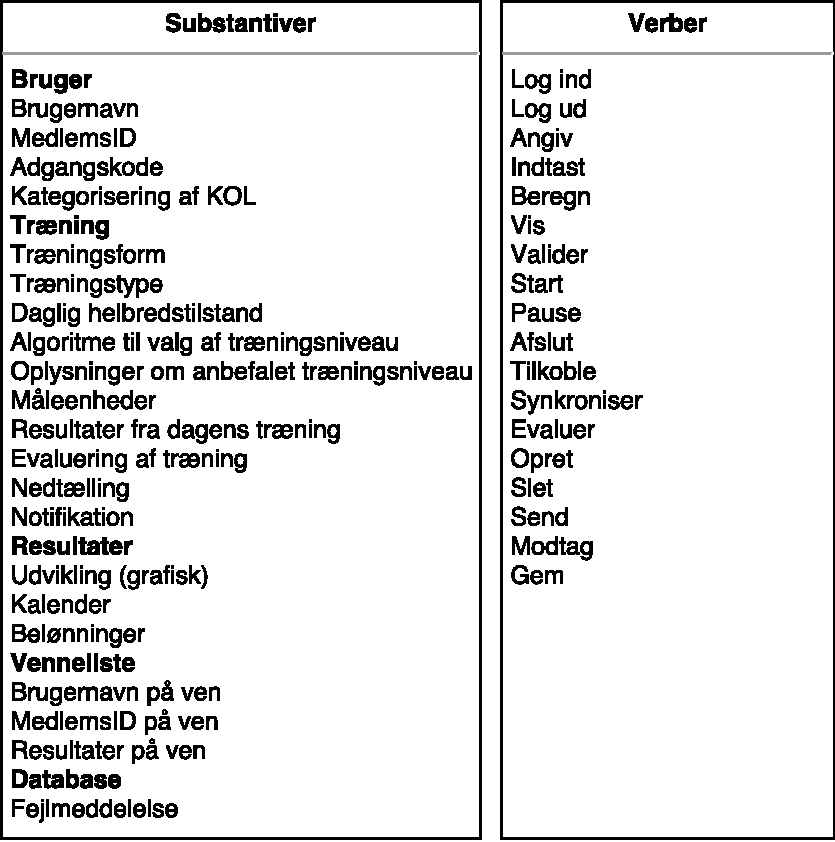
\includegraphics[width=1\textwidth]{figures/aktivitetsdiagram/substantiveverber}
\caption{Substantiver og verber identificeret ved analyse af systembeskrivelse, use case samt funktionaliteter.}
\label{tab:subverb}
\end{table}

\noindent
De fremhævede substantiver, brugeroplysninger, træning, resultater, venneliste og database, identificeres som klasser. Under hver klasse fremgår deres tilhørende attributter, der beskriver den overordnede klasse. Verberne betegner de metoder, der kan tilgås i de forskellige klasser. Klasserne er opstillet med relationer, hvilket fremgår af \autoref{fig:analyseklasse}.

\begin{figure}[H]
\centering
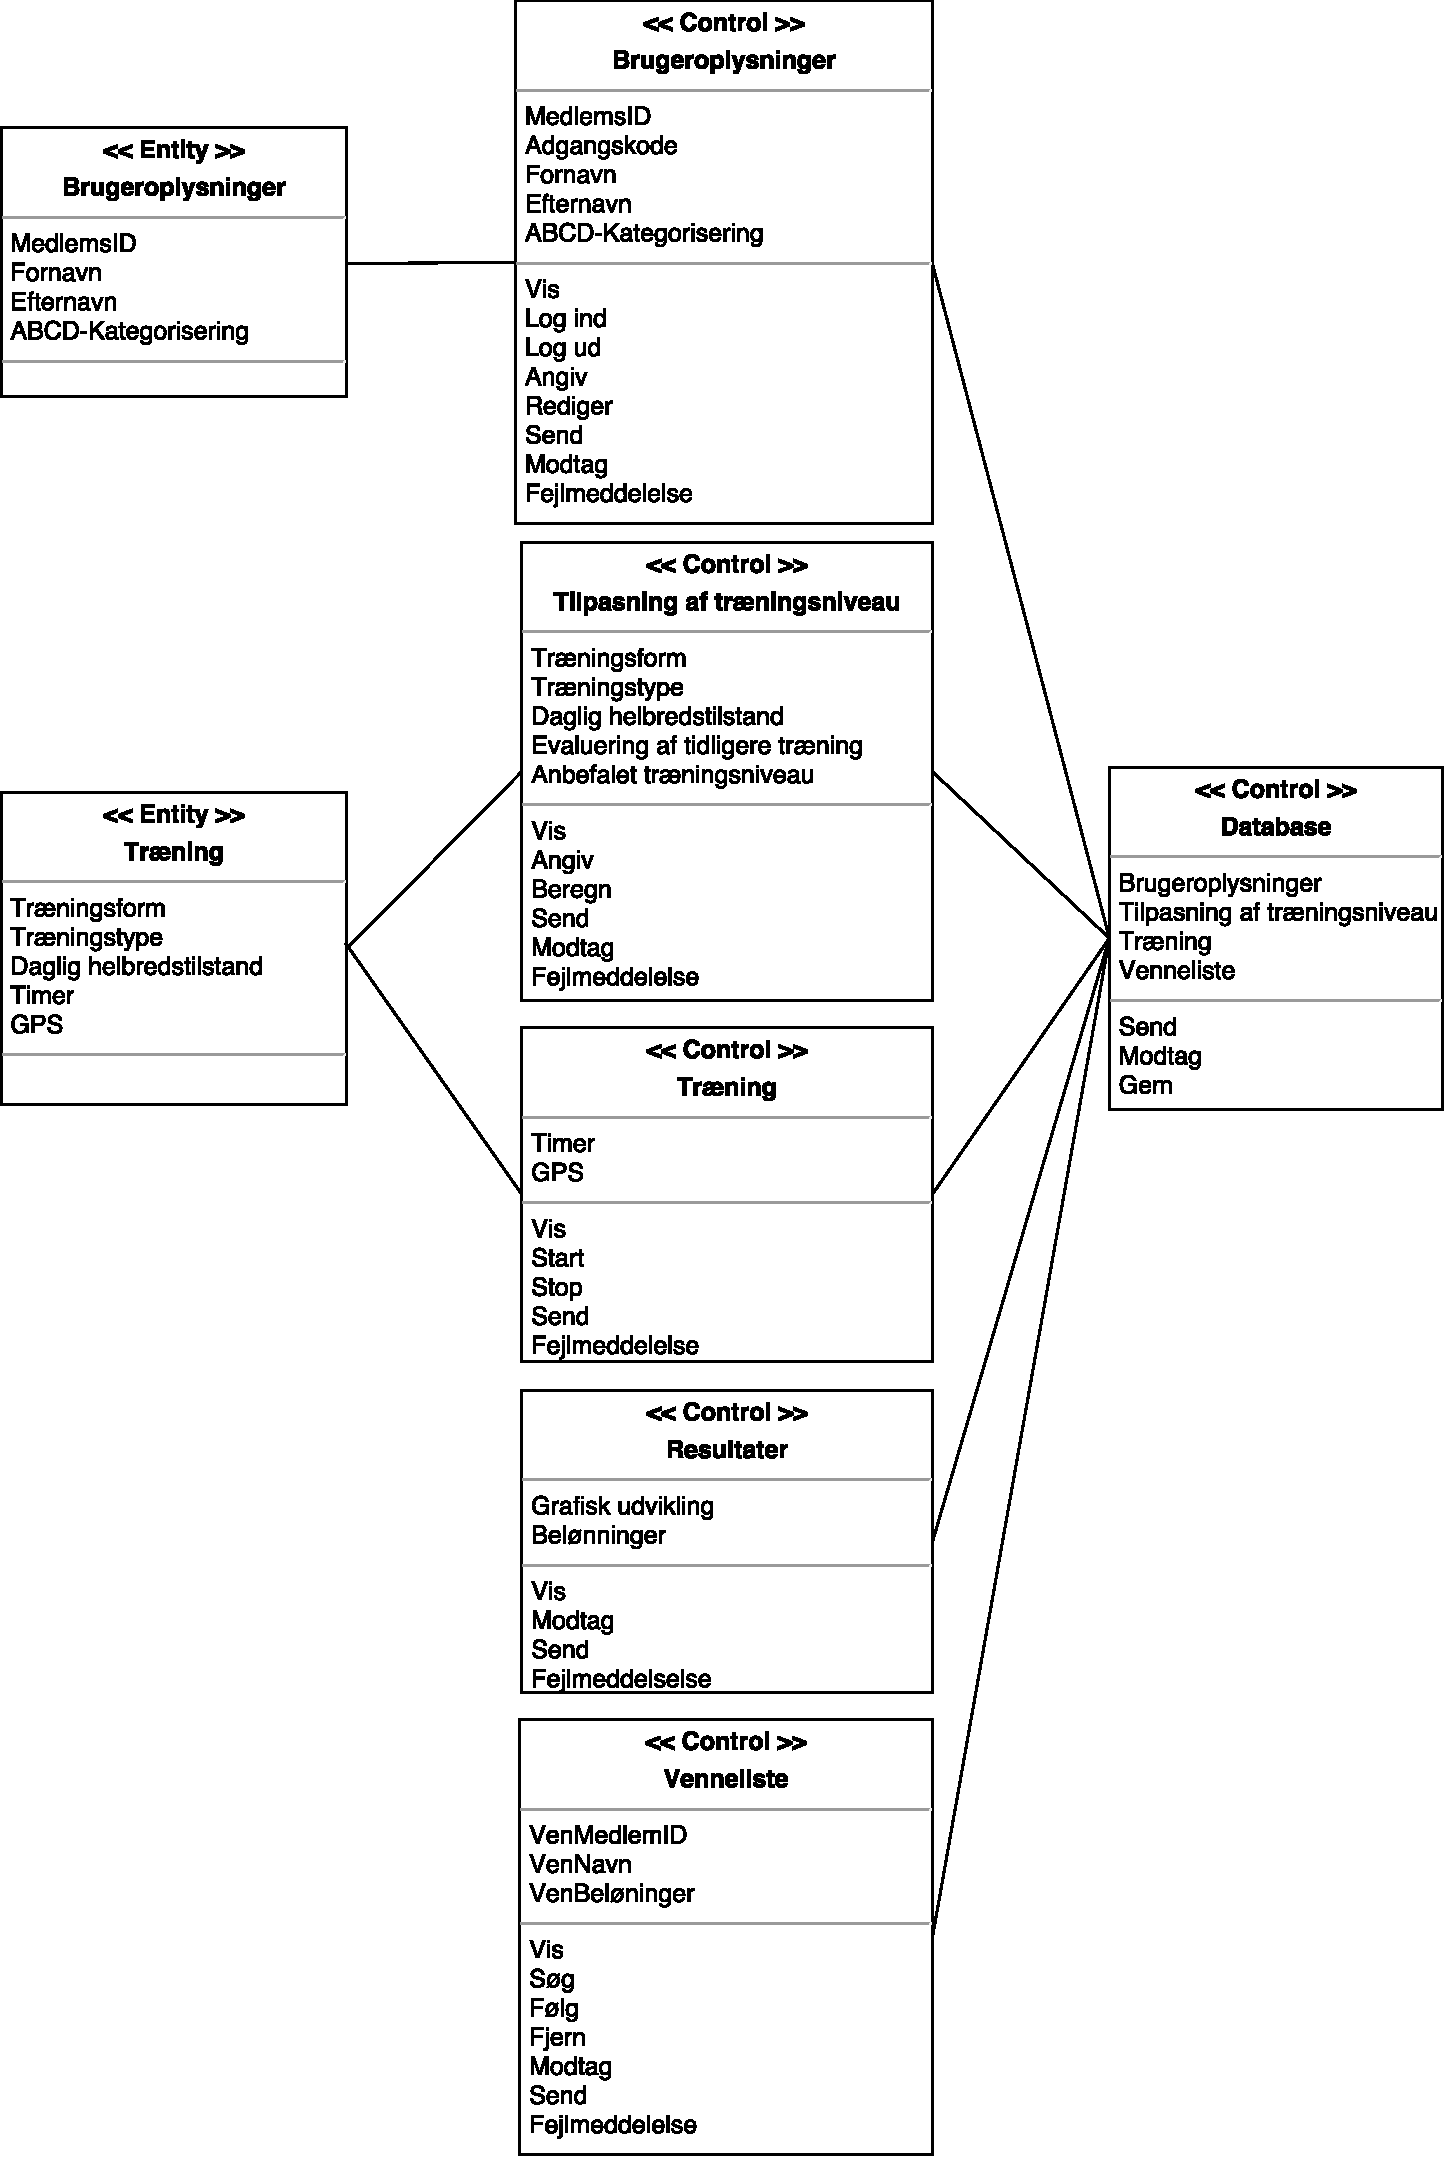
\includegraphics[width=1\textwidth]{figures/aktivitetsdiagram/analyseklasser}
\caption{Analyseklasser udarbejdet ud fra de identificerede substantiver og verber.}
\label{fig:analyseklasse}
\end{figure}

\noindent
Af \autoref{fig:analyseklasse} fremgår relationen mellem klasserne og deres dertilhørende attributter samt metoder. 



%%Afgrænsning
%%-----------------------Design-------------------------
\chapter{Systemdesign} \label{cha:design}
I dette kapitel beskrives design af app'en samt design af database. I design af app'en tages der udgangspunkt i de analyseklasser, der blev identificeret i \autoref{cha:analyse}, hvoraf disse omdannes til designklasser. Herefter visualiseres sammenspillet mellem de forskellige designklasser i sekvensdiagrammer. Design af database, der vil fremgå til sidst af kapitlet, vil visualiseres i et ER-diagram samt tilhørende schema. 

\section{Designafgrænsning} \label{sec:brugervenlighed}
Systemet designes med henblik på at opfylde kravsspecifikationerne, der blev udarbejdet i systemanalysen jf. \autoref{sec:funktionellekrav}. I forbindelse med de opstillede funktionelle krav foretages der afgrænsninger for at gøre design og efterfølgende implementering af systemet mere konkret. Der afgrænses til konditionstræning, da app'en formål ikke er at udforme et træningssæt til KOL-patienter. Dog forventes det, at implementeringen af styrketræning og vejrtrækningsøvelser er lignende. 

Der er opstillet et non-funktionelt krav om et brugervenligt system. For at opfylde dette krav, tages der udgangspunkt i gestaltlovene samt generelle egenskaber indenfor design af brugergrænseflader, der kan have indflydelse på brugervenligheden. 

Gestalt principperne bygger på en række love, der er opstillet af forskellige psykologer og anvendes til at designe visuelle elementer med henblik på forbedring af læring eller effektivisering af visuelle resultater. Der findes mange gestalt love. De mest anvendte til design af grænseflader er; symmetri, regelmæssighed, lukkethed, prægnans, fokuspunkt, ensartethed, nærhed, lighed og harmoni.\cite{Chang2002} Udover gestaltlovene har følgende egenskaber betydning for brugervenligheden \cite{ferre2001}:
\begin{itemize}
\item Systemets funktioner skal være lette at lære at anvende for uerfarne brugere.
\item Systemet skal være effektivt at anvende i forhold til tiden, det tager at fuldføre en opgave.
\item Det skal være let at huske, hvordan systemet anvendes efter længere perioder uden brug af systemet.
\item Fejlraten ved brug af systemet skal være så lav som muligt.
\item Systemet skal være tilfredsstillende for brugeren at anvende.
\end{itemize}
 

 






%% Designklasser
%\subsection{Brugervenlighed}
Der er i \autoref{sec:funktionellekrav} opstillet et non-funktionelt krav om et brugervenligt system. For at opfylde dette krav, tages der udgangspunkt i gestaltlovene samt generelle egenskaber indenfor design af brugergrænseflader, der kan have indflydelse på brugervenligheden. 

Gestalt principperne bygger på en række love, der er opstillet af forskellige psykologer og anvendes til at designe visuelle elementer med henblik på forbedring af læring eller effektivisering af visuelle resultater. Der findes mange gestalt love. De mest anvendte til design af brugergrænseflader er; symmetri, regelmæssighed, lukkethed, prægnans\fxnote{Figur-grund eller prægnans omhandler det psykologiske fænomen, at man ikke kan opleve en figur uden samtidig at opleve dens baggrund}, fokuspunkt, ensartethed, nærhed, lighed og harmoni.\cite{Chang2002} Udover gestalt lovene har følgende egenskaber betydning for brugervenligheden \cite{ferre2001}:
\begin{itemize}
\item Systemets funktioner skal være lette at lære at anvende for uerfarne brugere
\item Systemet skal være effektivt at anvende i forhold til tiden, det tager at fuldføre en opgave
\item Det skal være let at huske, hvordan systemet anvendes efter længere perioder uden brug af systemet
\item Fejlraten ved brug af systemet skal være så lav som muligt
\item Systemet skal være tilfredsstillende for brugeren at anvende
\end{itemize}
 
 
\section{Objektorienteret design}
Der vælges at opdele analyseklasserne, som tidligere er defineret, til mindre designklasser. Dette gøres for at specificere de definerede attributter og metoder, hvilket gør det lettere at modificere systemet. Ud fra de opstillede designklasser udarbejdes sekvensdiagrammer. I sekvensdiagrammerne er systemets klasser opdelt efter MVC. Objektet og livslinjer farvekodes afhængig af klassens MVC-type. Modelklasser er røde, viewklasser er blå, og controllerklasser er grønne. I sekvensdiagrammer findes desuden også database, som er illustreret med lilla. I sekvensdiagrammerne findes metoder, der henter data fra en klasse til en anden. Idet det ikke er en egentlig metode, der sender data, illustreres overførslen med en stiplet pil, når data sendes til en klasse efter en hent-metode er kaldt. 

Der er udarbejdet et samlet diagram over designklasser og relationerne i mellem, hvilket vil fremgå af bilag \autoref{bilagA}. De enkelte designklasser og sekvensdiagrammer er opdelt i database, lagring af data, fejlmeddelelse, log ind, kategorisering, hovedmenu, tilpasning af træningsniveau, træning, resultater, venneliste, redigering af adgangskode og log ud. 

\subsection{Database}
Databasen kan tilgås ved den tilhørende controller. Databasen og controlleren fremgår af \autoref{fig:MVCDatabase}. 

\begin{figure} [H]
\centering
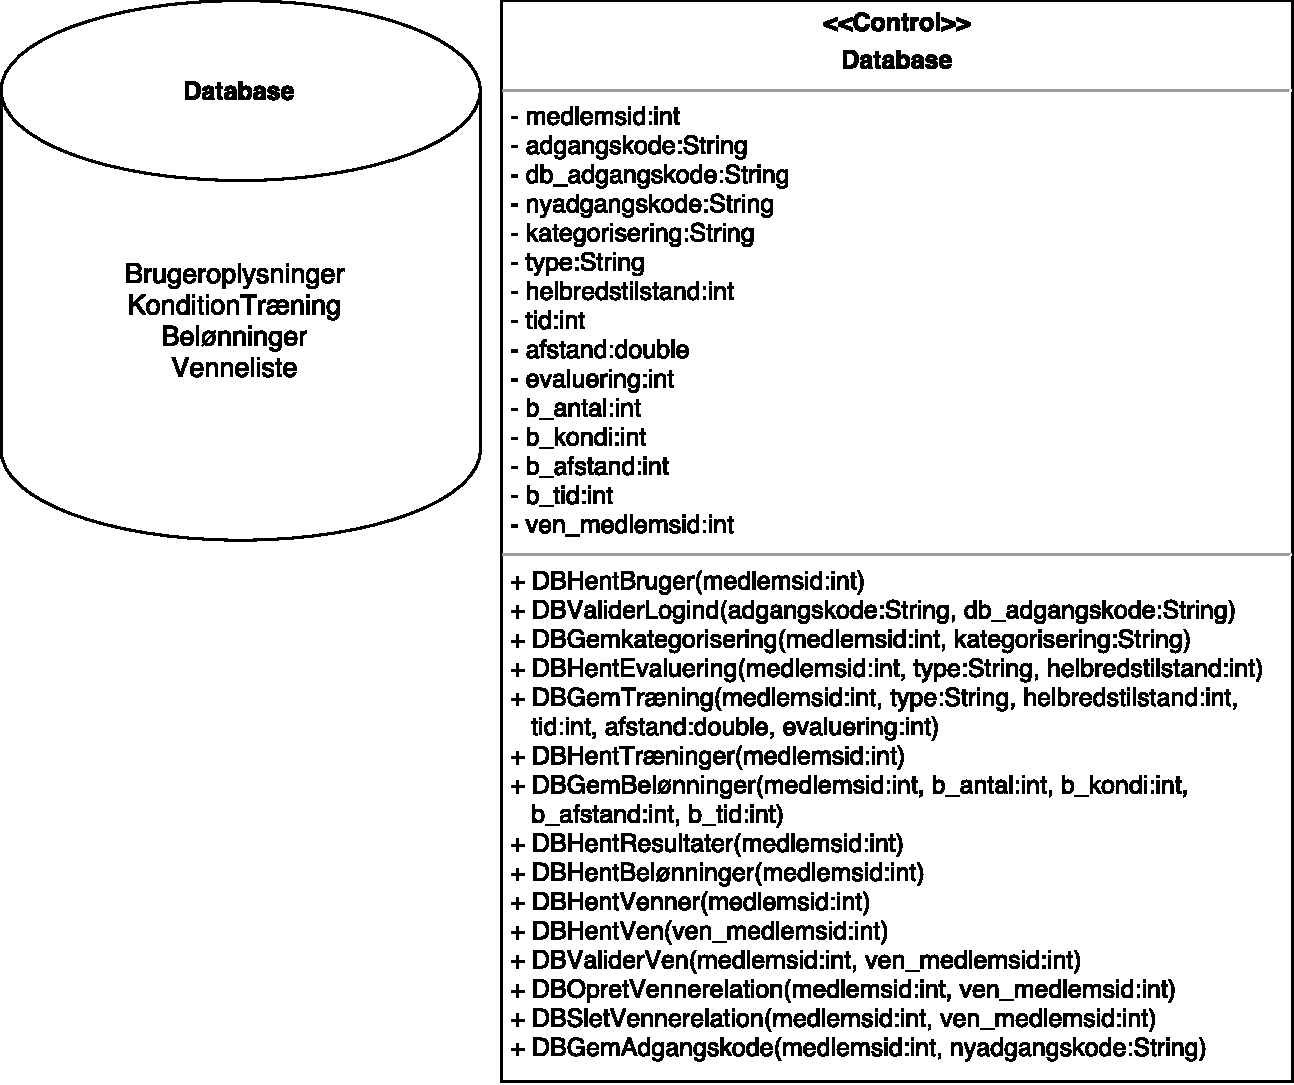
\includegraphics[width=0.9\textwidth]{figures/MVC/MVCDatabase}
\caption{Designklasser for Database.}
\label{fig:MVCDatabase}
\end{figure}

\noindent
Databasen indeholder brugeroplysninger, venneliste, resultater og registrerede brugere. Designet af denne vil fremgå af \autoref{sec:ER}. \textit{DatabaseController} har til formål at gemme, sende og modtage data mellem databasen og de forskellige controllere. Der oprettes forbindelse til denne ved log ind, hvor brugeroplysninger, venneliste og resultater sendes og gemmes i de forskellige entity. 


\subsection{Entity}  
Databasen har oprettet forbindelse ved log ind, sendes og gemmes data i tre forskellige entity, som fremgår af \autoref{fig:MVCEntity}. 

\begin{figure} [H]
\centering
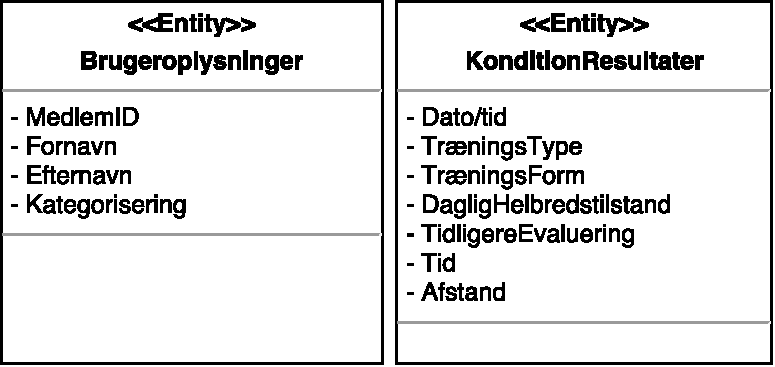
\includegraphics[width=0.9\textwidth]{figures/MVC/Entity}
\caption{Designklasser for Entity.}
\label{fig:MVCEntity}
\end{figure}

\noindent
\textit{Brugeroplysninger} indeholder informationer om brugeren, herunder MedlemsID, Adgangskode, Fornavn, Efternavn og Kategorisering. Denne har en relation med RedigeringController, som fremgår af \autoref{fig:MVCRedigering}. 
\textit{Venneliste} har informationer om andre brugere der følges, såsom VenMedlemsID, VenFornavn, VenEfternavn og VenBelønninger. Controllerne der har relationen til denne beskrives i \autoref{fig:MVCVenneliste} og  \autoref{fig:MVCVen}.
\textit{Resultater} indeholder brugerens resultater, som er defineret ud fra DatoTid, TræningsType, TræningsForm, DagligHelbredstilstand, Evaluering, Tid, Afstand, EksterneMålinger og Belønninger. Disse har relation til ResultatController, der fremgår af  \autoref{MVCResultat}.


\subsection*{Fejlmeddelelse}
Til at vise fejlmeddelelser er der opstillet en fælles grænseflade, hvori teksten ændres alt efter, hvilken fejl, der forekommer. Designklassen ses af \autoref{fig:Designfejl}.

\begin{figure} [H]
\centering
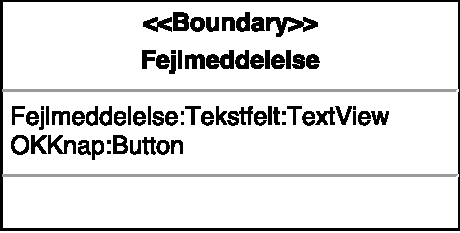
\includegraphics[width=0.5\textwidth]{figures/MVC/MVCfejl}
\caption{Designklasse for fejlmeddelelse.}
\label{fig:Designfejl}
\end{figure}

\noindent
Grænsefladen indeholder, foruden et tekstfelt, en OKKnap, der ved tryk henviser systemet til den forhenværende grænseflade. Fejlmeddelelsesgrænsefladen håndteres af den pågældende controller, hvori fejlen opstår. 
\input{rapportAfsnit/eProblemloesning/Design/MVCLogind}
\subsection*{Kategorisering}
Kategoriseringsfunktionen inddeles i klasser af typen boundary og en dertilhørende controller, som det fremgår af \autoref{fig:DesignKategorisering}.

\begin{figure} [H]
\centering
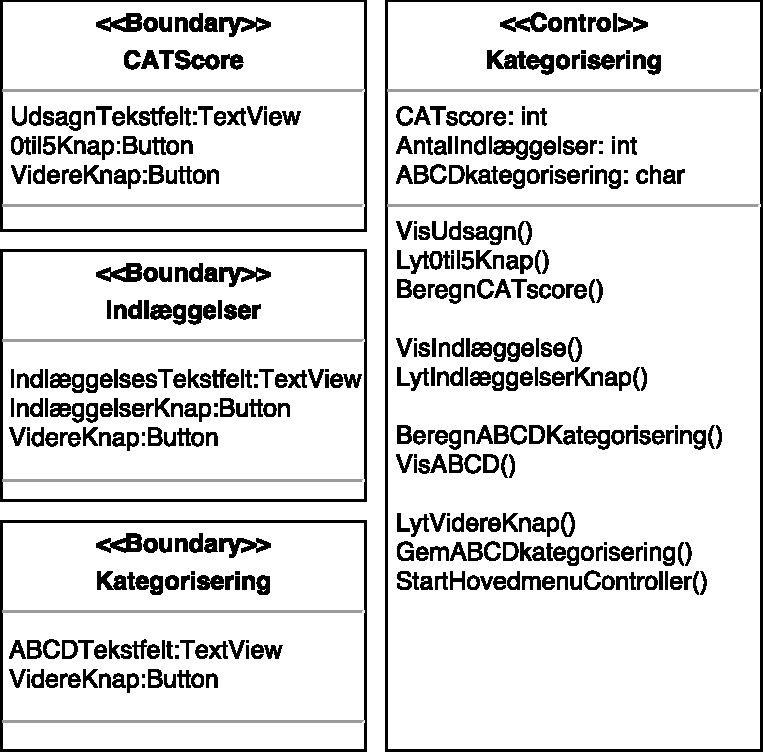
\includegraphics[width=0.9\textwidth]{figures/MVC/MVCKategorisering}
\caption{Designklasser for kategorisering.}
\label{fig:DesignKategorisering}
\end{figure}

\noindent
I \textit{KategoriseringGrænseflade} stilles otte udsagn fra CAT-scoren, som besvares af brugeren ved hjælp af knapper af typen button. Dertil fremgår der ligeledes en videre knap for således, at brugeren kan bekræfte sit svar og fortsætte til næste udsagn. Efter udsagnene er besvaret, skal indlæggelser det seneste år forårsaget af KOL besvares ud fra to yderligere knapper. Når kategoriseringen er beregnet vises denne i et tekstfelt. 

\textit{KategoriseringController} håndterer de forskellige knapper samt beregning af kategoriseringen ud fra den samlede CAT-score og antal indlæggelser. Kontrolleren lytter efter knapperne til besvarelse af de otte udsagn samt indlæggelser. Efter kategoriseringen er beregnet sendes denne til databasen, hvorefter den gemmes. Dertil har kontrolleren metoden til at starte hovedmenuen efter gennemført kategorisering.  
\subsection*{Hovedmenu} \label{sec:MVCHovedmenu}
Hovedmenuen er den primære grænseflade, der inddeles i en boundary samt en tilhørende controller. Disse fremgår af \autoref{fig:Designhovedmenu}.

\begin{figure} [H]
\centering
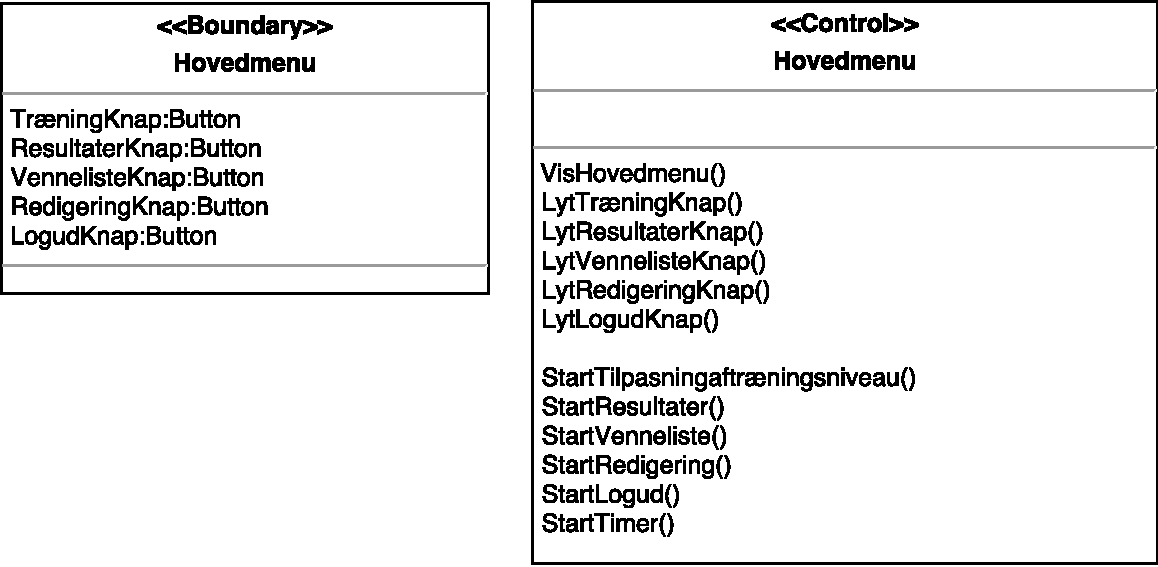
\includegraphics[width=0.9\textwidth]{figures/MVC/MVCHovedmenu}
\caption{Designklasser for hovedmenu.}
\label{fig:Designhovedmenu}
\end{figure}

\noindent
\textit{HovedmenuGrænseflade} skal tillade adgang til de forskellige funktionaliteter af app’en, herunder skal det være muligt at tilgå træning, resultater, venneliste, redigering samt log ud. Funktionaliteterne tilgås via tilhørende knapper af typen button. 

Til grænsefladen er der ligeledes en \textit{HovedmenuController}, som viser layoutet for hovedmenuen. Controlleren lytter derudover efter de forskellige knapper, hvorefter den respektive metode startes.  

\subsection*{Tilpasning af træningsniveau}
Førend en træning kan påbegyndes, tilpasses træningsniveauet den enkelte bruger. Tilpasning af træningsniveauet er inddelt i fire boundarys. Disse håndteres af en samlet controller, hvilket fremgår af \autoref{fig:DesignTilpasning}.

\begin{figure} [H]
\centering
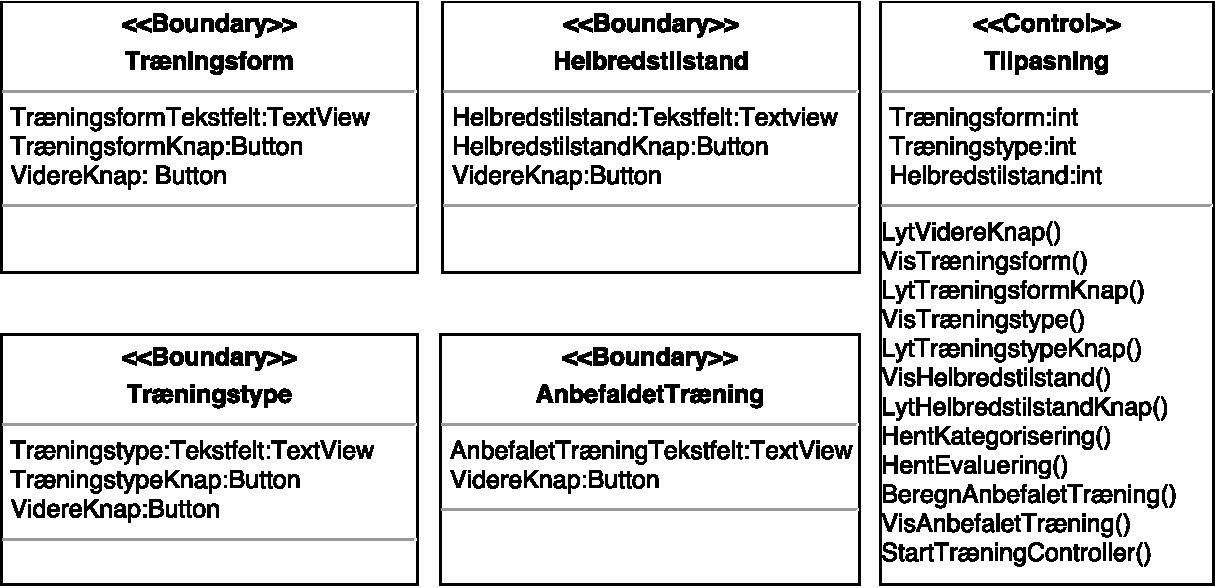
\includegraphics[width=1\textwidth]{figures/MVC/MVCTilpasning}
\caption{Designklasser for tilpasning af træningsniveau. Til venstre ses de fire boundarys for henholdsvis Træningsform, Træningstype, Helbredstilstand og AnbefaletTræning. Til højre fremgår den tilhørende controller.}
\label{fig:DesignTilpasning}
\end{figure}

\noindent
Der er opstillet grænseflader for tilpasning af træning, hvilket omfatter \textit{Træningsform}, \textit{Træningstype}, \textit{Helbredstilstand} og \textit{AnbefaletTræning}. Der er til hver grænseflade opstillet tekstfelter af typen TextView og knapper af typen Button.   

Den tilhørende controller til de ovenstående boundarys lagrer den angivne træningsform, træningstype samt helbredstilstand  i entityen, KonditionResultater, således disse senere kan sendes til databasen efter endt træning. Der er opstillet tilhørende private attributter og metoder, herunder Vis, Lyt, Send, Hent, Beregn og Start. Metoderne sender, henter og beregner i forhold til definerede inputsparametre. Efter inputsparametre er der angivet, hvorvidt der returneres en værdi.

I sammenspil med designklasserne er der udarbejdet et sekvensdiagram, hvilket fremgår af \autoref{fig:SEKTilpasning}. 

\begin{figure} [H]
\centering
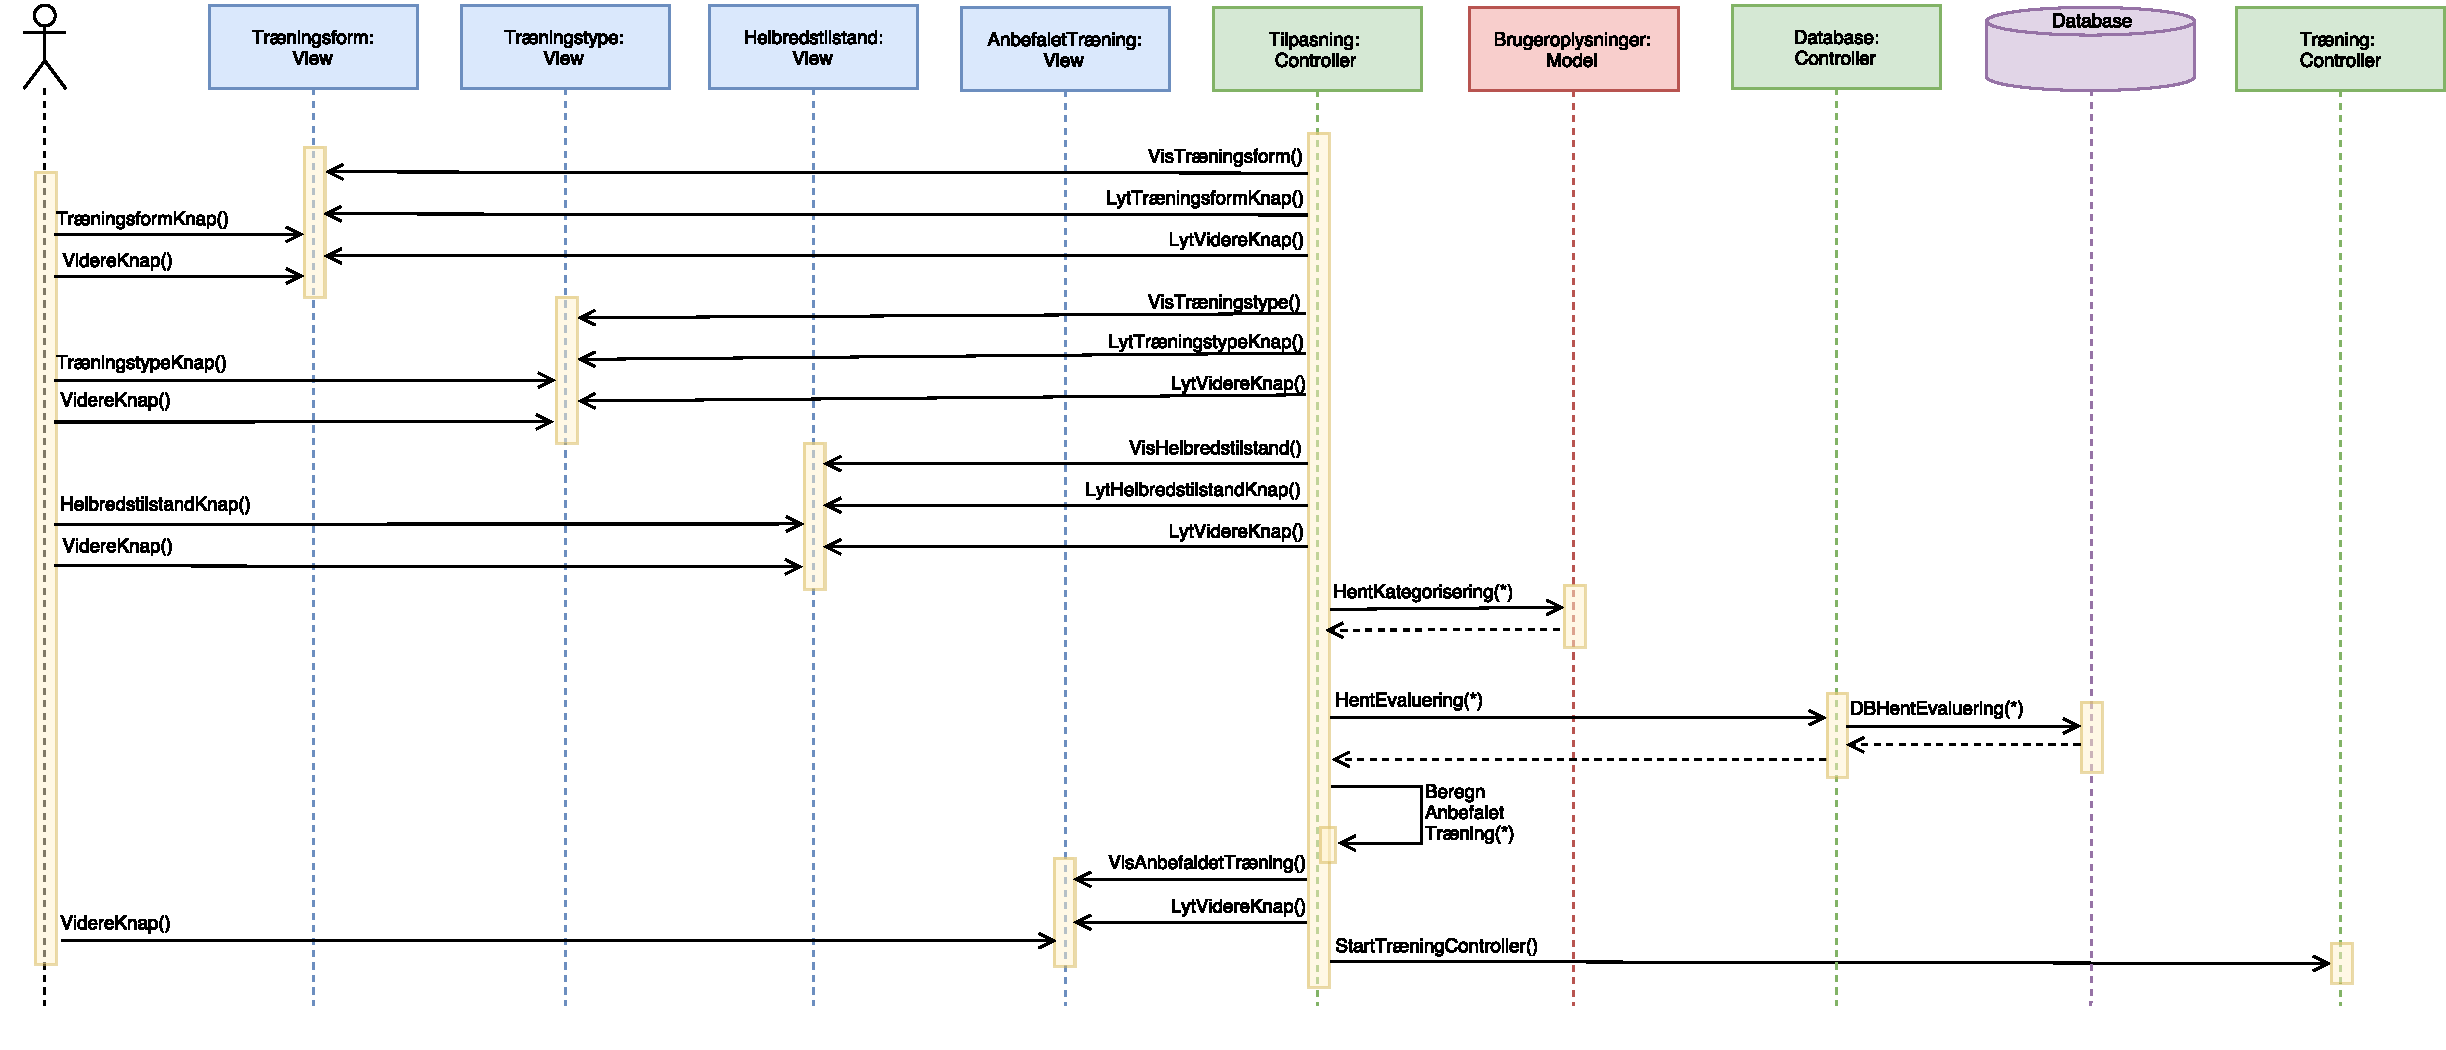
\includegraphics[width=1.55\textwidth, angle=90]{figures/Sek/SEKTilpasning}
\caption{Sekvensdiagram for tilpasning af træningsniveau.}
\label{fig:SEKTilpasning}
\end{figure}

\noindent
Den første grænseflade, som vises, er \textit{Træningsform}. Denne grænseflade indeholder et tekstfelt, der beskriver, hvad brugeren skal angive. Dertil er der opstillet en TræningsformKnap, hvor brugeren kan vælge mellem konditionstræning, styrketræning eller vejrtrækningsøvelser. Når der er angivet træningsform, trykker brugeren på VidereKnap, hvorefter controlleren, \textit{Tilpasning}, viser grænsefladen for valg af \textit{Træningstype}. Brugeren skal her angive træningstype ud fra tre forskellige muligheder. Dette vil for eksempel ved konditionstræning være gå, løbe eller cykle. Brugeren bekræfter valget ved at trykke på VidereKnap, hvorefter controlleren viser grænsefladen for \textit{Helbredstilstand}. Helbredstilstanden angives og bekræftes ved at trykke på VidereKnap. Herefter sender controlleren parametrene, type og helbredstilstand, til modellen \textit{KonditionResultater}, hvorefter controlleren henter kategoriseringen i modellen for \textit{Brugeroplysninger} og efterfølgende tidligere evaluering fra \textit{Database} via \textit{Database} controlleren, hvis der eksisterer en tilhørende evaluering. Stjerner indikerer inputsparametre, der fremgår af tilhørende designklasse.
Efterfølgende beregner controlleren \textit{Tilpasning} anbefalet træningsniveau og viser dette på grænsefladen for \textit{AnbefaletTræning}. Brugeren kan herefter trykke på VidereKnap, hvis denne trykkes på, startes \textit{Træning} controlleren. 

\subsection*{Træning}
Træningen er opdelt i tre boundarys. Boundaryen \textit{Evaluering} er først aktiv efter træningen, idet træningen skal evalueres. Der er til disse tre boundarys opstillet en fælles controller. Boundarys og controller fremgår af \autoref{fig:DesignTraening}. 

\begin{figure} [H]
\centering
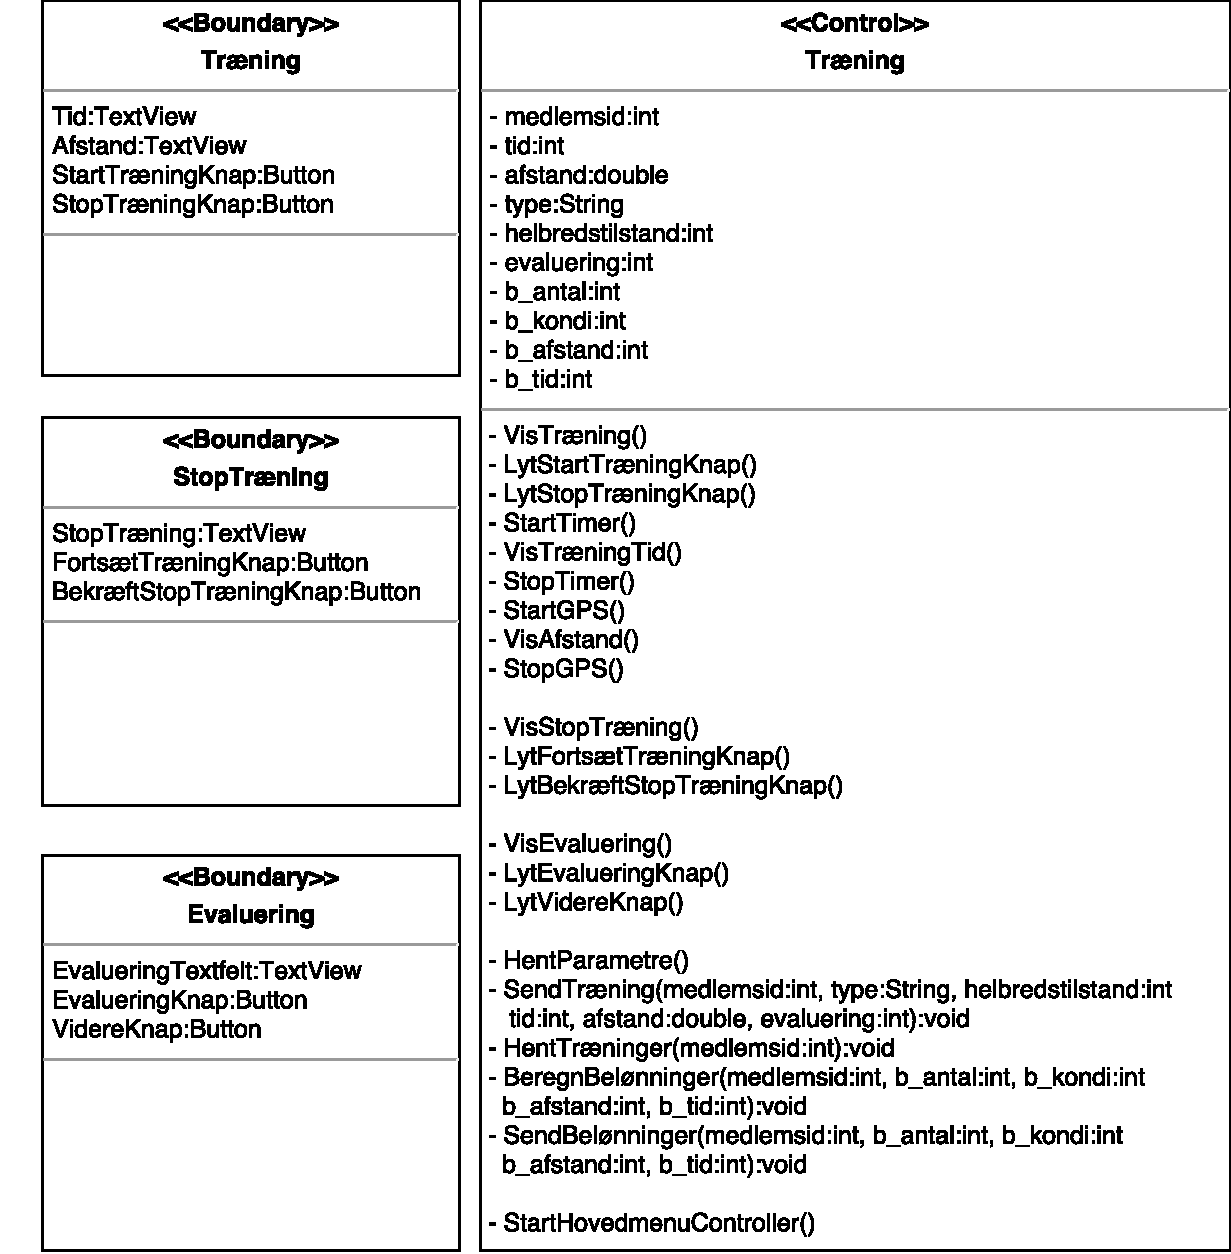
\includegraphics[width=0.7\textwidth]{figures/MVC/MVCTraening}
\caption{Designklasser for træning samt evaluering. Til venstre fremgår boundarys for Træning, StopTræning og Evaluering. Den tilhørende controller ses til højre.}
\label{fig:DesignTraening}
\end{figure}

\noindent
Grænsefladen for \textit{Træning}, \textit{StopTræning} og \textit{Evaluering} indeholder tekstfelter og knapper af typen TextView og Button. Controlleren \textit{TræningEvaluering} indeholder metoderne Lyt, Vis, Start, Stop og Send. 

I sammenspil med designklasserne er der udarbejdet et sekvensdiagram, hvilket fremgår af \autoref{fig:SEKTraening}. 

\begin{figure} [H]
\centering
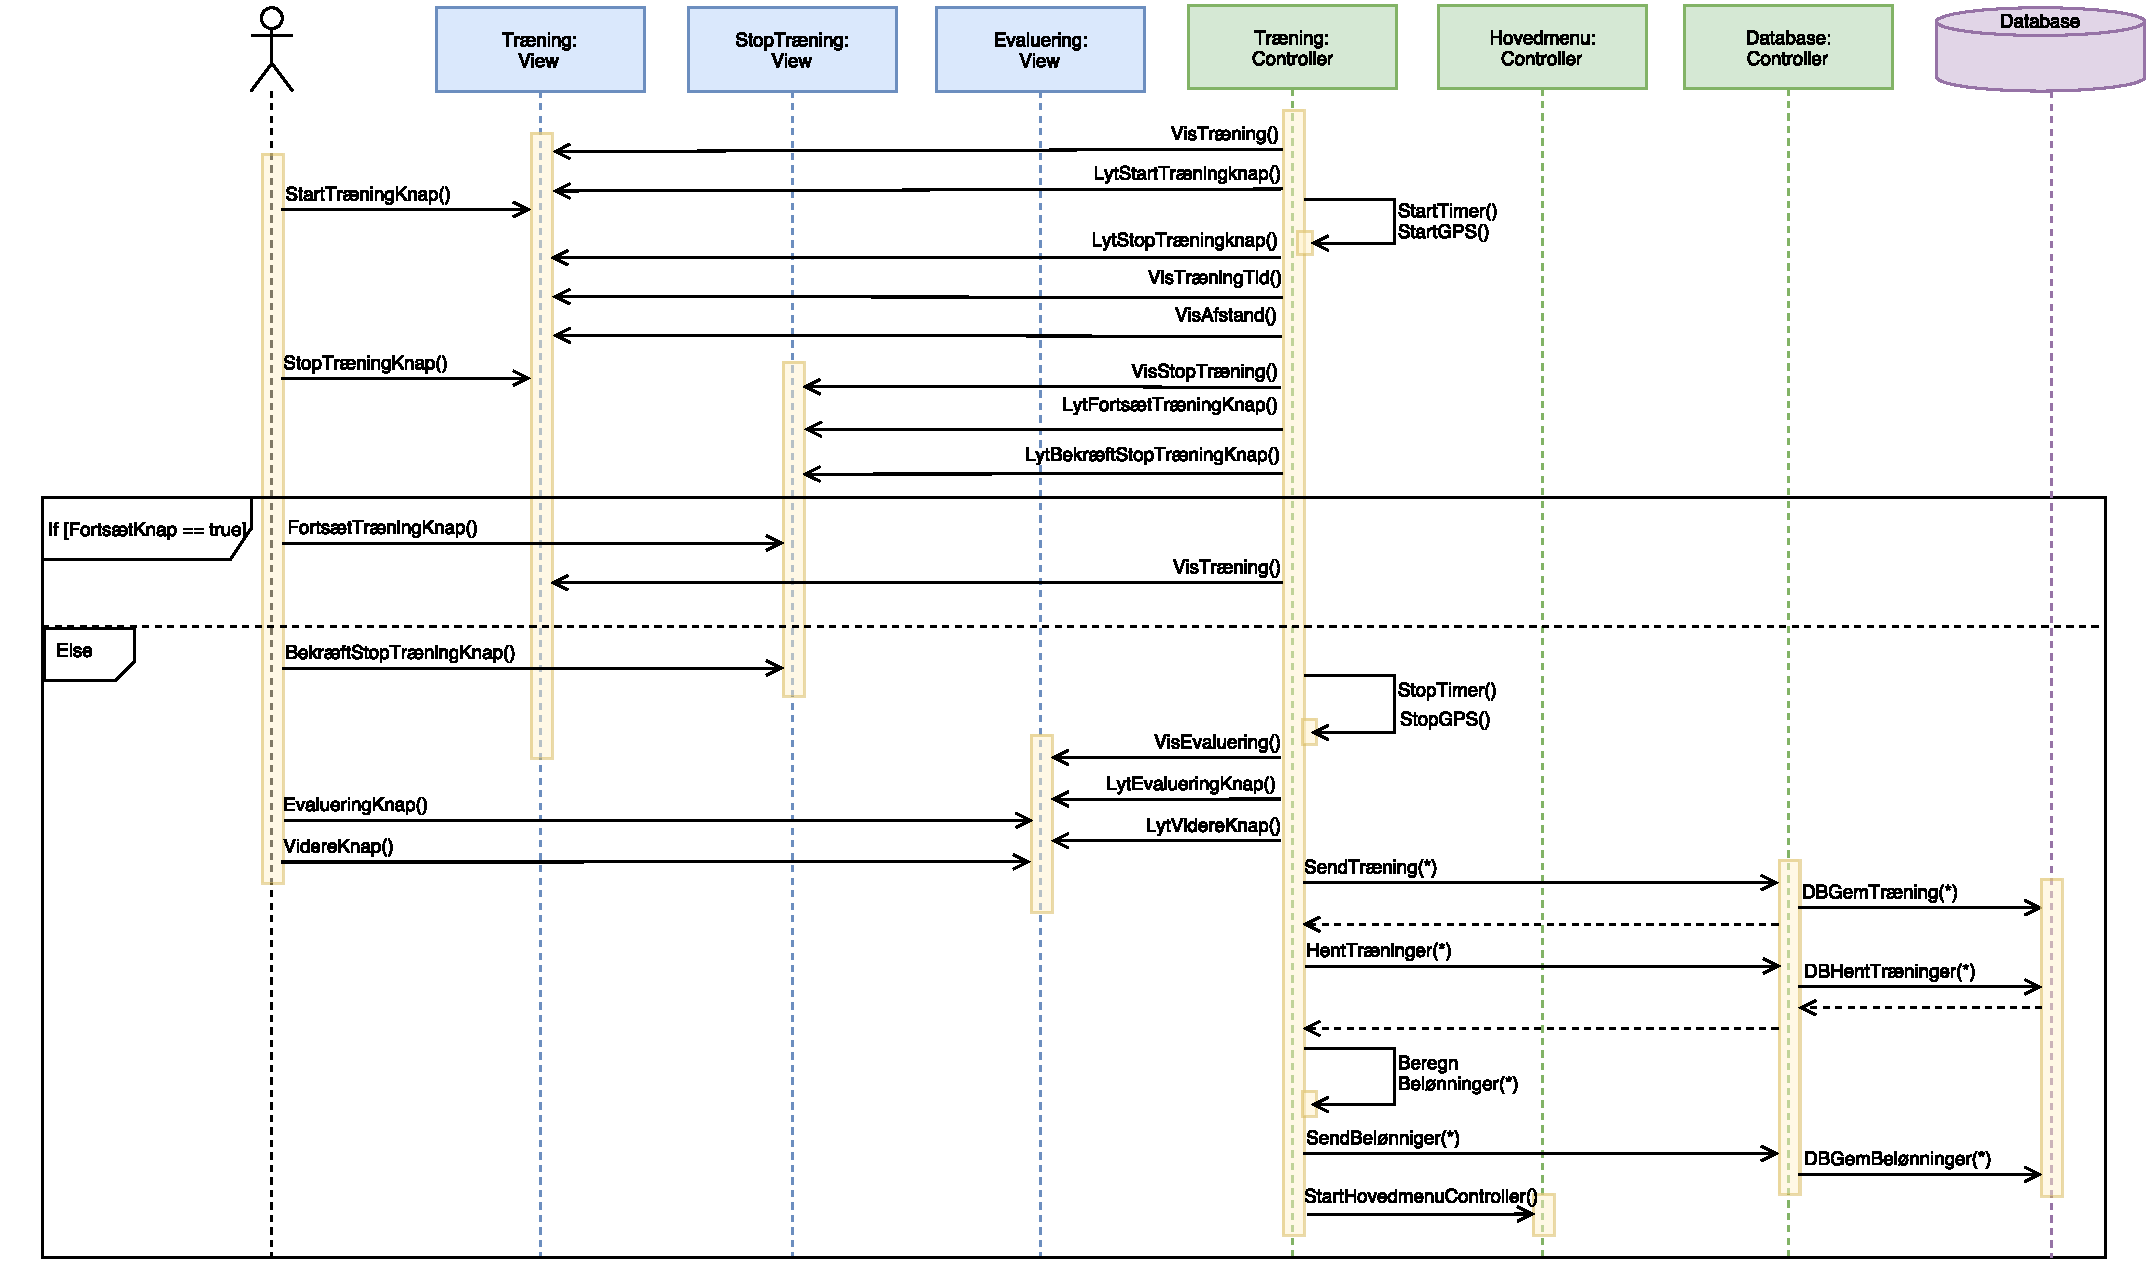
\includegraphics[width=1.55\textwidth, angle=90]{figures/Sek/SEKTraening}
\caption{Sekvensdiagram for træning.}
\label{fig:SEKTraening}
\end{figure}

\noindent
\textit{Træning} er den første grænseflade, der vises efter tilpasningen af træningsniveauet. Controlleren \textit{TræningEvaluering} starter timer og GPS, når brugeren har trykket på StartTræningKnap. Herefter vises tiden og afstanden i grænsefladen. Brugeren kan under træningen, eller når træningen er fuldført, afslutte ved at trykke på StopTræningKnap, hvorefter grænsefladen for \textit{StopTræning} vises. I denne grænseflade har brugeren mulighed for at trykke på FortsætTræningKnap eller BekræftStopTræningKnap. Vælges FortsætTræningKnap vises grænsefladen for \textit{Træning}, og brugeren skal igen trykke på StartTræningKnap for at starte træning og måleenheder. Vælges BekræftStopTræningKnap stopper controlleren med at måle data fra GPS og timer. Herefter vises grænsefladen \textit{Evaluering}, hvor brugeren skal angive en evaluering af dagens træning. Evaluering bekræftes ved VidereKnap. Herefter sender controlleren træningsoplysninger til controlleren for \textit{Database}, som gemmer træningen i \textit{Database}. Der gives besked til \textit{Hovedmenu} controlleren om at vise hovedmenuen.



%Denne indeholder tekstfelter, hvori tiden samt afstanden oplyses. Derudover er der et tekstfelt til kompatiblemålinger, hvis disse er tilsluttet. Da \textit{TræningsGrænsefladen} skal oplyse målinger fra tilkoblede kompatible måleenheder, skal denne grænseflade ligeledes styres af \textit{TilkoblingafkompatibleenhederController}, der ses af \autoref{fig:kompatiblemåleenheder}. Yderligere indeholder denne grænseflade en stopknap, af typen button, hvis træningen ønskes afsluttet. 
%Ønskes træningen afsluttet vises \textit{StopTræningGrænseflade}, hvori der er opstillet et tekstfelt samt to knapper. Tekstfeltet informerer brugeren om, at vedkommende er ved at afslutte træningen, hvorved brugeren kan bekræfte, at træningen skal stoppes eller fortsætte træningen ved hjælp af de opstillede knapper. 
%Efter en afsluttet træning, skal træningen evalueres, hvilket forekommer i \textit{EvalueringGrænsefladen}. Denne grænseflade indeholder et tekstfelt, der informerer brugeren om evalueringen, samt fire knapper. De tre knapper er opstillet således brugeren kan evaluere den udførte træning. Evalueringen bekræftes ved, at benytte den sidste knap til at bevæge sig videre i app’en. 
%\textit{TræningEvalueringController} er den fælles controller, som bestemmer, hvilken boundary, som vises. Denne controller lagrer tiden, afstanden, evaluering samt kompatible målinger, hvis disse er tilkoblet. Derudover lytter controlleren på de forskellige respektive knapper og håndterer skiftet mellem boundarys. Idet brugeren har evalueret sin træning og bekræftet ved at benytte videreknappen sendes alle træningsoplysningerne til databasen, hvori de gemmes. Dertil returneres brugeren til hovedmenuen. 

\subsection{Resultater}
Resultater inddeles i en grænseflade og dertilhørende controller, som det fremgår af \autoref{fig:MVCresultater}. 

\begin{figure} [H]
\centering
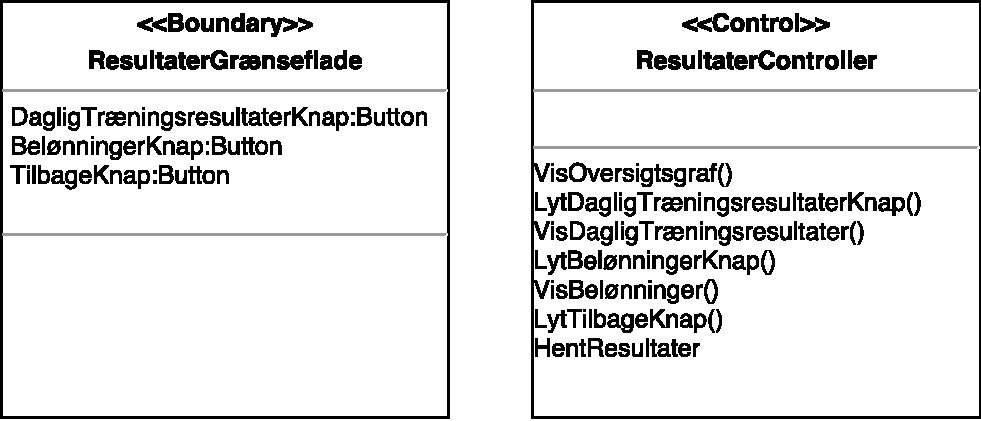
\includegraphics[width=0.9\textwidth]{figures/MVC/Resultater}
\caption{Designklasser for resultater}
\label{fig:MVCresultater}
\end{figure}

\noindent
I \textit{ResultaterGrænseflade} er der opstillet knapper af typen button for daglig træningsresultater belønninger og en tilbage. Disse indikerer ved tryk, at brugerens har valgt en af de mulige handlinger. 
 
Der er til \textit{ResultaterGrænseflade} opstillet en \textit{ResultatController}, der har til formål at hente nye resultater fra dagens træning i træningscontrolleren, når resultater tilgås via hovedmenugrænsefladen. Herefter vises en oversigtsgraf over udført træning. Træningscontrolleren fremgår af \autoref{fig:MVCTræning}. Controlleren lytter på om brugeren trykker på de angivne knapper i grænsefladen for resultater og viser valgt handling, hvis dette er tilfældet. 

\subsection*{Venneliste}
Venneliste inddeles i to boundaryklasser og en dertilhørende controlklasse, som fremgår af \autoref{fig:MVCVenneliste}. 

\begin{figure} [H]
\centering
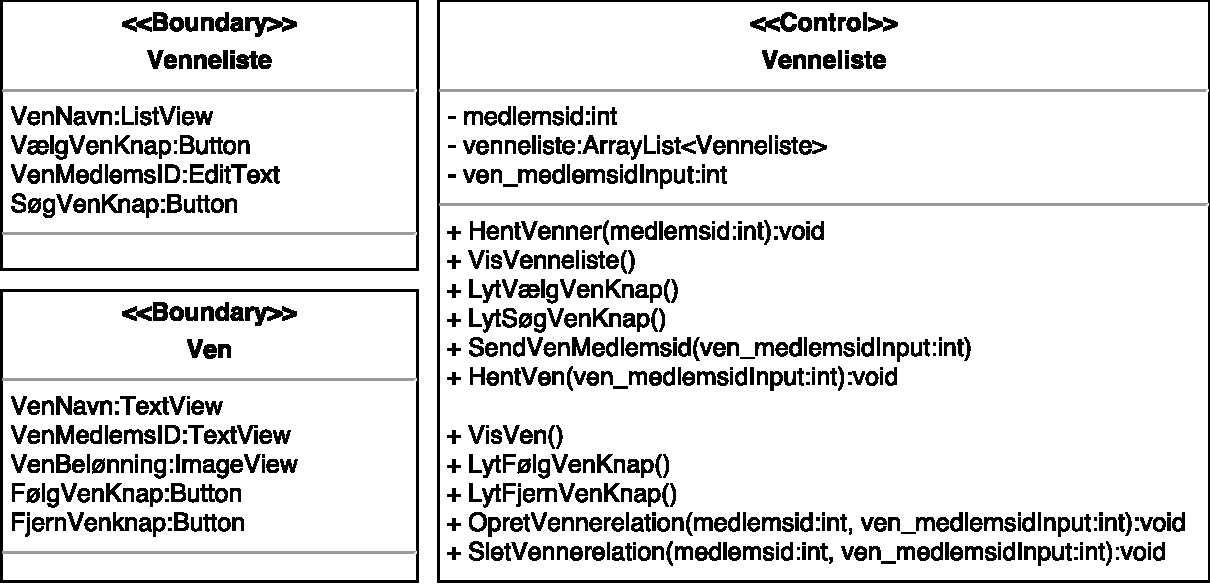
\includegraphics[width=0.5\textwidth]{figures/MVC/MVCVenneliste}
\caption{Designklasser for venneliste. Til venstre ses boundary for Venneliste og Ven, hvor der til højre ses tilhørende controller.}
\label{fig:MVCVenneliste}
\end{figure}

\noindent
I grænsefladen \textit{Venneliste} findes en liste, af typen ListView, med navn på de brugere, der følges. Hver bruger, der vises af den givne grænseflade, kan tilgås ved at trykke på brugeren. Derudover er der i denne grænseflade et søgefelt, af typen EditText, med en tilhørende SøgVenKnap, af typen Button, som muliggør, at brugeren kan søge på andre brugere med deres medlemsID. 
Når en bruger tilgås, enten via vennelisten eller ved at søge på en bruger, vises grænsefladen for den pågældende bruger. Hertil vises  tekstfelter, af typen TextView, med brugerens medlemsID og navn, samt et billede af typen ImageView, som viser brugerens belønninger. Hvis brugeren ikke følges, er der her opstillet en FølgVenKnap.
Den tilhørende controller har metoderne Hent, Vis, Lyt og Opret. 
Ud fra de nævnte designklasser er udarbejdet et sekvensdiagram, der fremgår af \autoref{fig:SEKVenneliste}.

\begin{figure} [H]
\centering
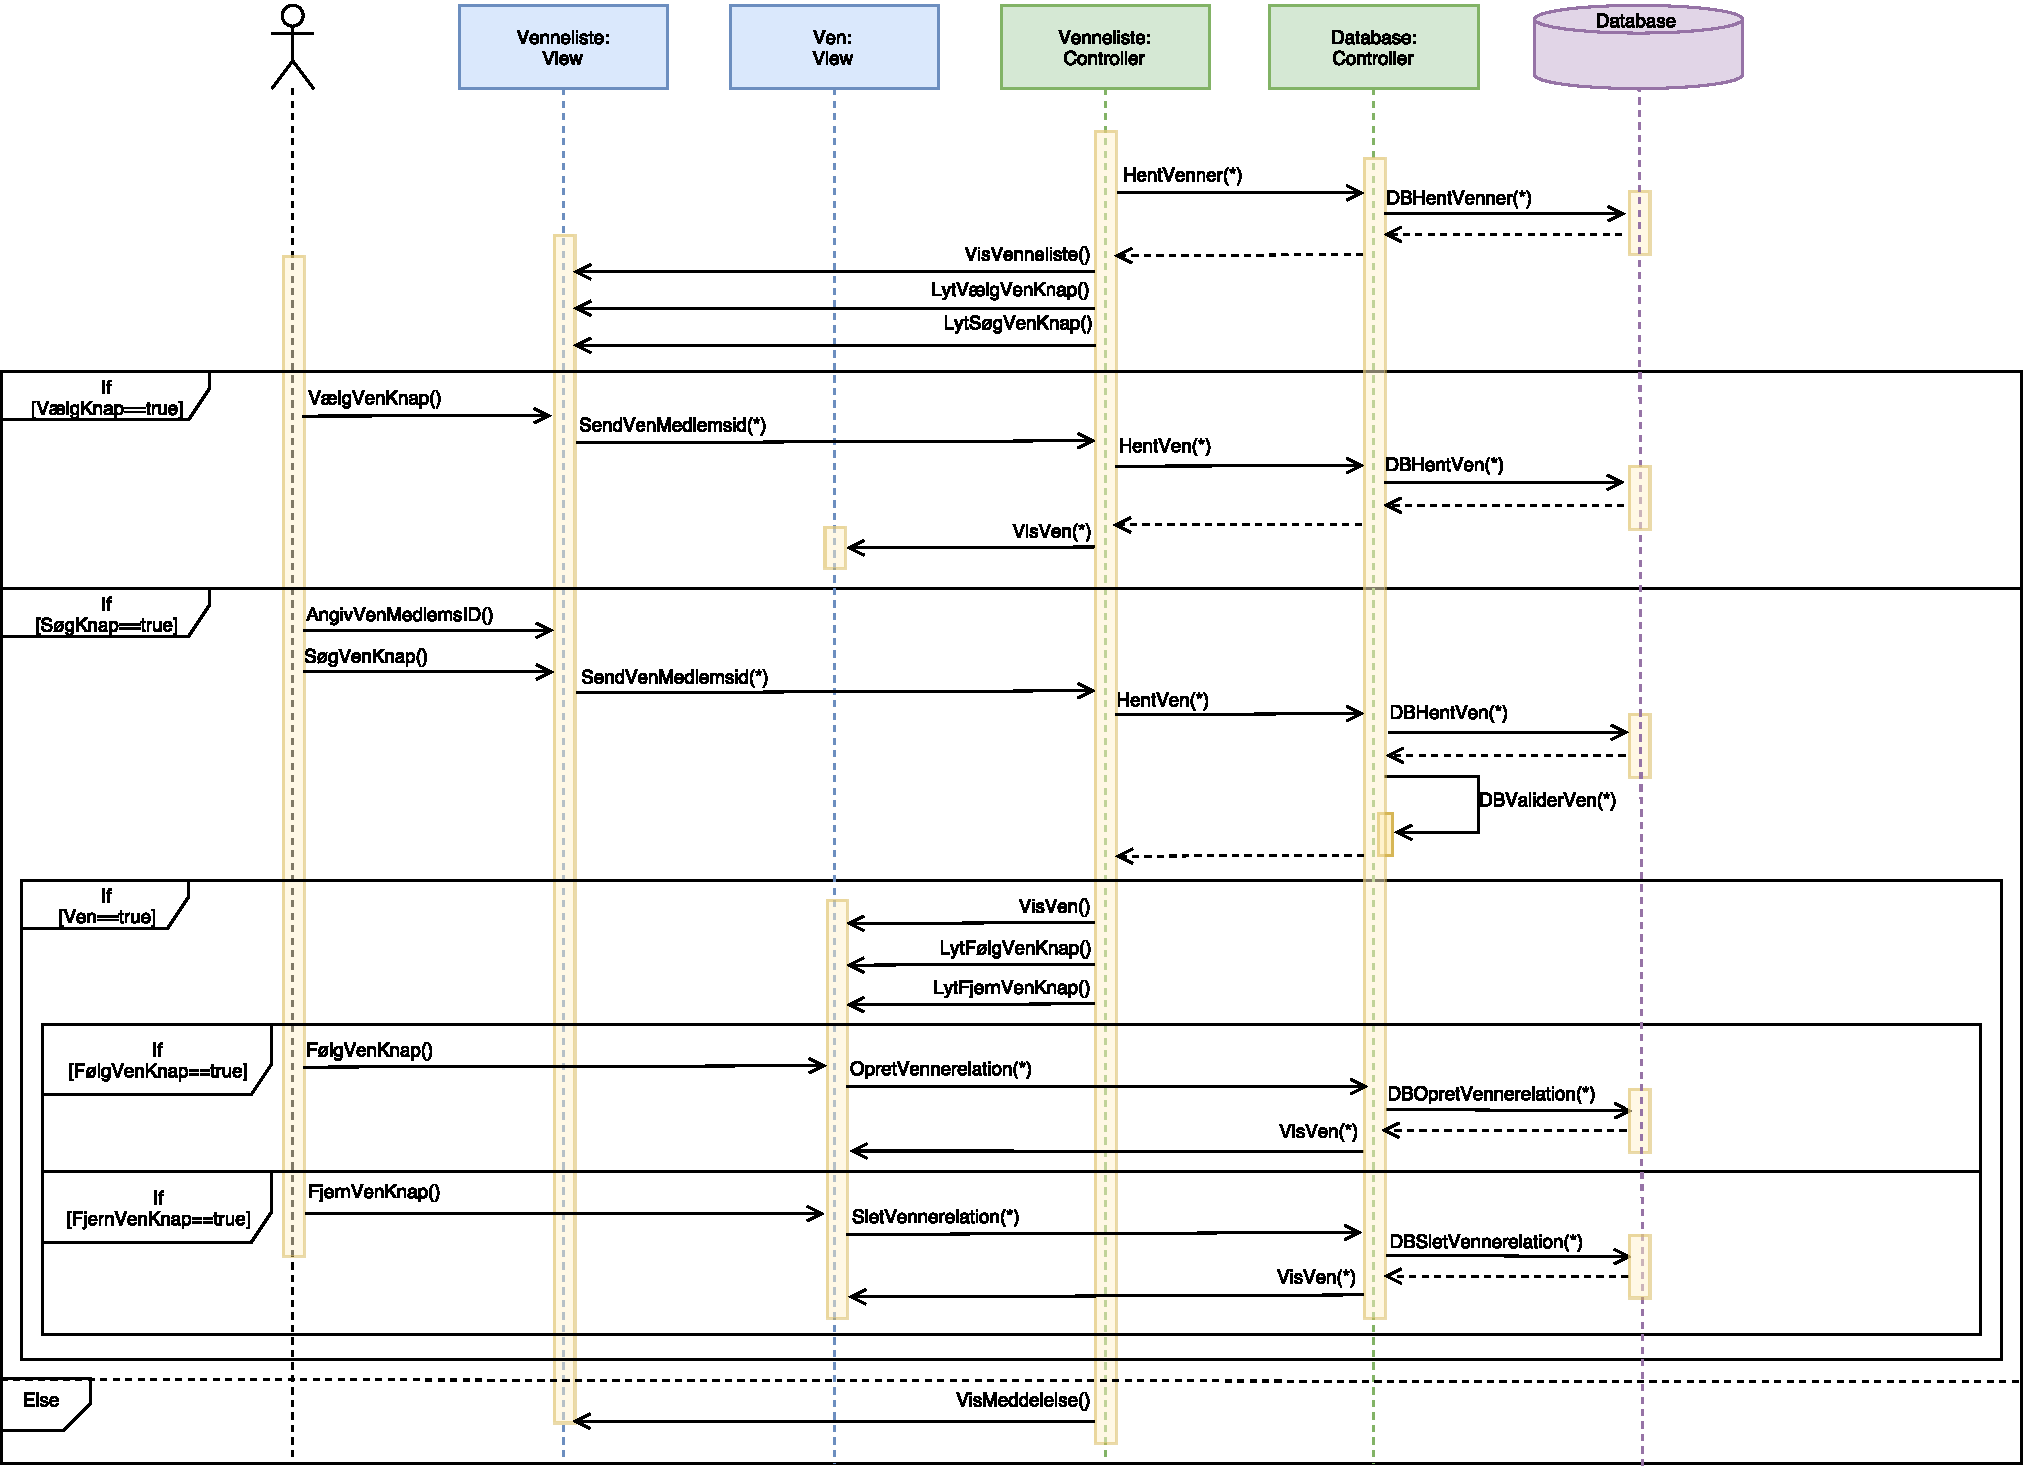
\includegraphics[width=1.55\textwidth, angle=90]{figures/Sek/SEKVenneliste}
\caption{Sekvensdiagram for venneliste.}
\label{fig:SEKVenneliste}
\end{figure}

\noindent
Controlleren \textit{Venneliste} henter venneliste fra \textit{Database} via dens tilhørende controller, hvorefter grænsefladen for venneliste vises. 
Dertil lytter controlleren på VælgVenKnap samt SøgVenKnap. Vælger brugeren at tilgå en ven fra vennelisten, vises grænsefladen for den valgte ven. Vælger brugeren derimod at søge efter en anden bruger, hentes det indskrevne medlemsID, således den søgte bruger kan findes i databasen, hvortil den valideres. Såfremt brugeren ikke findes i databasen vises en grænseflade for \textit{Fejlmeddelelse} og brugeren returneres efterfølgende til grænsefladen for \textit{Venneliste}. Findes brugeren i databasen vises grænsefladen \textit{Ven}, hvor brugeren har mulighed for at følge vennen. Hvis brugeren trykker på FølgVenKnap oprettes der en vennerelation i databasen. Brugeren vil efterfølgende fremgå af vennelisten.  



%Venneliste inddeles i en grænseflade og dertilhørende controller, som det fremgår af \autoref{fig:MVCVenneliste}. 

%\begin{figure} [H]
%\centering
%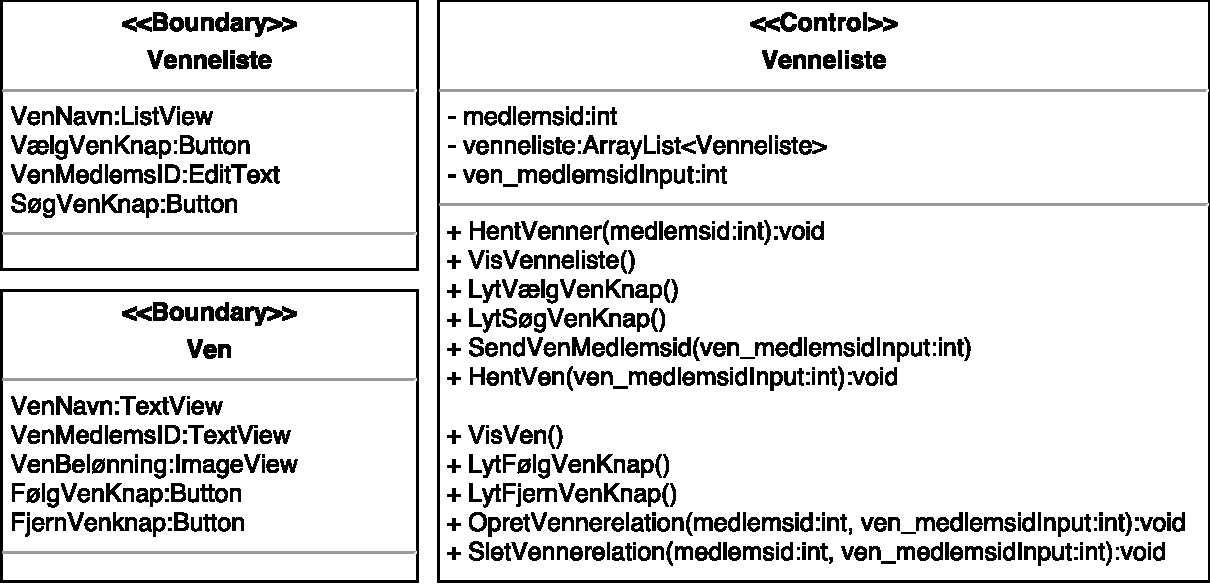
\includegraphics[width=0.8\textwidth]{figures/MVC/MVCVenneliste}
%\caption{Designklasser for venneliste.}
%\label{fig:MVCVenneliste}
%\end{figure}

%\noindent
%\textit{VennelisteGrænsefladen} indeholder tekstfelter for fornavn og efternavn på de brugere de følger. Derudover er der opstillet tekstfelt for medlemsID, hvor brugeren kan angive medlemsID'et på en bruger de ønsker at følge. Dertil er der opstillet en tilhørende søge knap, af typen button, der ved tryk indikere at brugeren har angivet medlemsID på brugeren den ønsker at følge. Derudover har brugeren mulighed for at vælge en bruger eller gå tilbage via en vælg eller tilbage  knap, der også er af typen button. 


%Der er til \textit{VennelisteGrænsefladen} opstillet en \textit{VennelisteController}, der har til formål at vise en oversigt over vennelisten når grænsefladen for vennelisten tilgås. Brugeren har via vælg knappen mulighed for at tilgå en bruger den følger
%Controlleren lytter på om brugeren trykker på vælg knappen eller søg knappen. Vælg knappen giver brugeren mulighed for at tilgå enkelt bruger ud fra vennelisten. Trykker brugeren på søg knappen kontrollere controlleren om det angivne medlemsID findes i databasen, herefter kan brugeren trykke på vælg. Trykkes der på en af vælg knapperne, enten i vennelisten eller efter søgning på medlemsID vises \textit{VenGrænsefladen}, som fremgår af \autoref{MVCVen}. Controlleren lytter på tilbage knappen, hvis denne trykkes på vises forrige grænseflade. 


%\subsubsection*{Ven}
%Ven inddeles i en grænseflade og tilhørende controller, som det fremgår af \autoref{fig:MVCVen}.

%\begin{figure} [H]
%\centering
%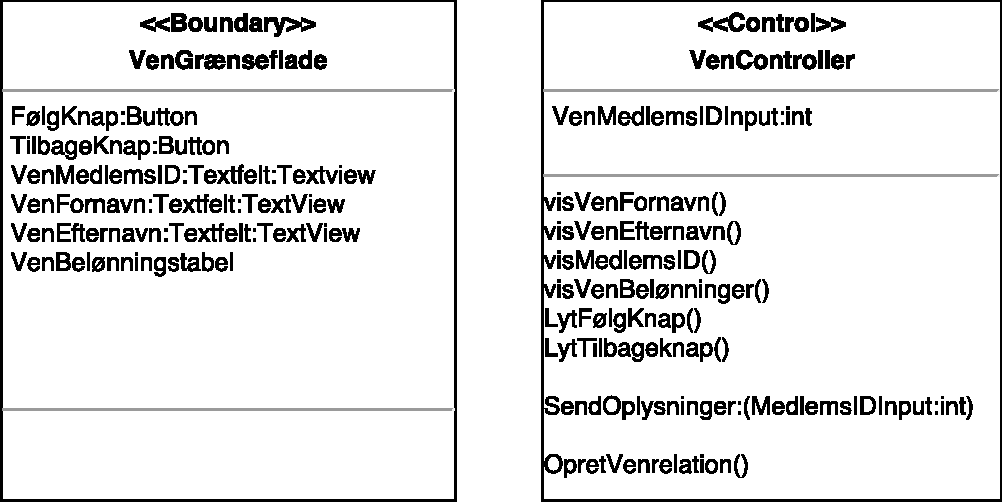
\includegraphics[width=0.8\textwidth]{figures/MVC/MVCVen}
%\caption{Designklasser for ven.}
%\label{fig:MVCVen}
%\end{figure}

%\noindent
%I \textit{VenGrænseflade} vises tekstfelter for valgt bruger, herunder MedlemsID, fornavn og efternavn. Dertil er der opstillet en følg knap og en tilbage knap af typen button. Følg knap er kun tilgængelig, hvis brugeren ikke følger den valgte ven. Derudover vises en tabel med den valgte brugers belønninger.


%Til \textit{VenGrænsefladen} er der opstillet en \textit{VenController}, som har til formål vise brugeroplysninger, herunder MedlemsID, fornavn og efternavn samt belønningstabel for den valgte bruger. Controlleren lytter på om brugeren trykker på følg knappen, hvis brugeren ikke allerede følger eller trykker på tilbage knappen. Trykkes der på følg knappen sendes MedlemsID'et på den bruger der ønskes at følges til databasen, hvorefter vennerelation gemmes i denne. Vælger brugeren at trykke på tilbage knappen vises den forrige grænseflade.   
\subsection{Redigering}
Redigering inddeles i en grænseflade og en tilhørende controller, som det fremgår af \autoref{fig:Redigering}. 

\begin{figure} [H]
\centering
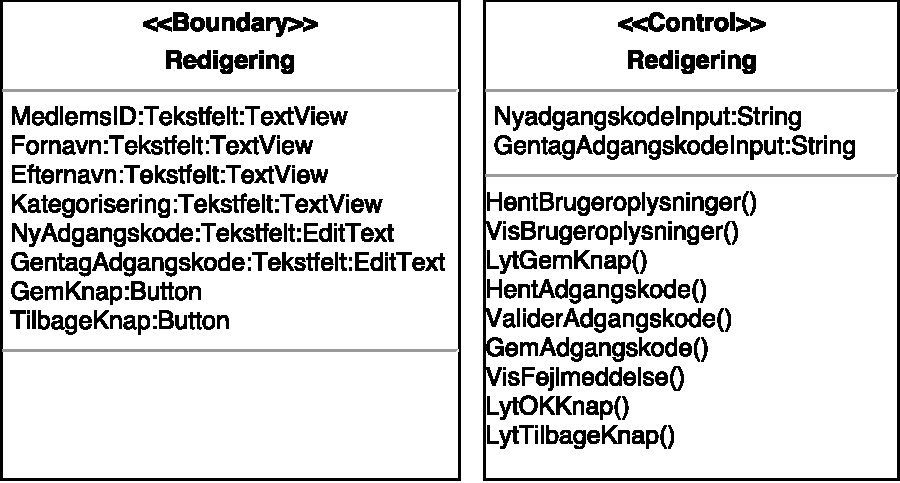
\includegraphics[width=0.9\textwidth]{figures/MVC/Redigering}
\caption{Designklasser for Redigering.}
\label{fig:Redigering}
\end{figure}


\noindent
I \textit{RedigeringGrænseflade} opstilles tekstfelter for medlemsID, fornavn, efternavn og kategorisering. Derudover opstilles tekstfelter for ny adgangskode og gentag adgangskode, hvor brugeren kan redigere adgangskoden. Dertil er der en gem knap og en tilbage knap, af typen button. Gem knappen indikere ved tryk at brugeren ønsker at gemme den nye adgangskode. 


Til \textit{RedigeringGrænsefladen} er der opstillet en \textit{RedigeringController}, som har til formål at vise informationer om brugeren. Derudover lytter den på gem knappen, hvis denne trykkes, sammenligner controlleren de indtastede adgangskoder. Er disse ens sender controlleren den  nye adgangskode til databasen. Controlleren lytter på om tilbage knappen trykkes på, hvis dette sker vises den forrige grænseflade.  


\section*{Log ud}
Log ud inddeles i en boundary og en dertilhørende controller, som det fremgår af \autoref{fig:MVCLogUd}. 

\begin{figure} [H]
\centering
\includegraphics[width=0.6\textwidth]{figures/MVC/Logud}
\caption{Designklasser for log ud. Til venstre ses boundary og til højre controller.}
\label{fig:MVCLogUd}
\end{figure}

\noindent
Der opstilles i log ud et tekstfelt, af typen TextView. Dertil opstilles en BekræftKnap og FortrydKnap af typen Button. 
Den tilhørende controller indeholder metoderne, Vis, Lyt, Nulstil og Start. I sammenspil med designklasserne er der opstillet et sekvensdiagram, som fremgår af \autoref{fig:SEKlogUd}.

\begin{figure} [H]
\centering
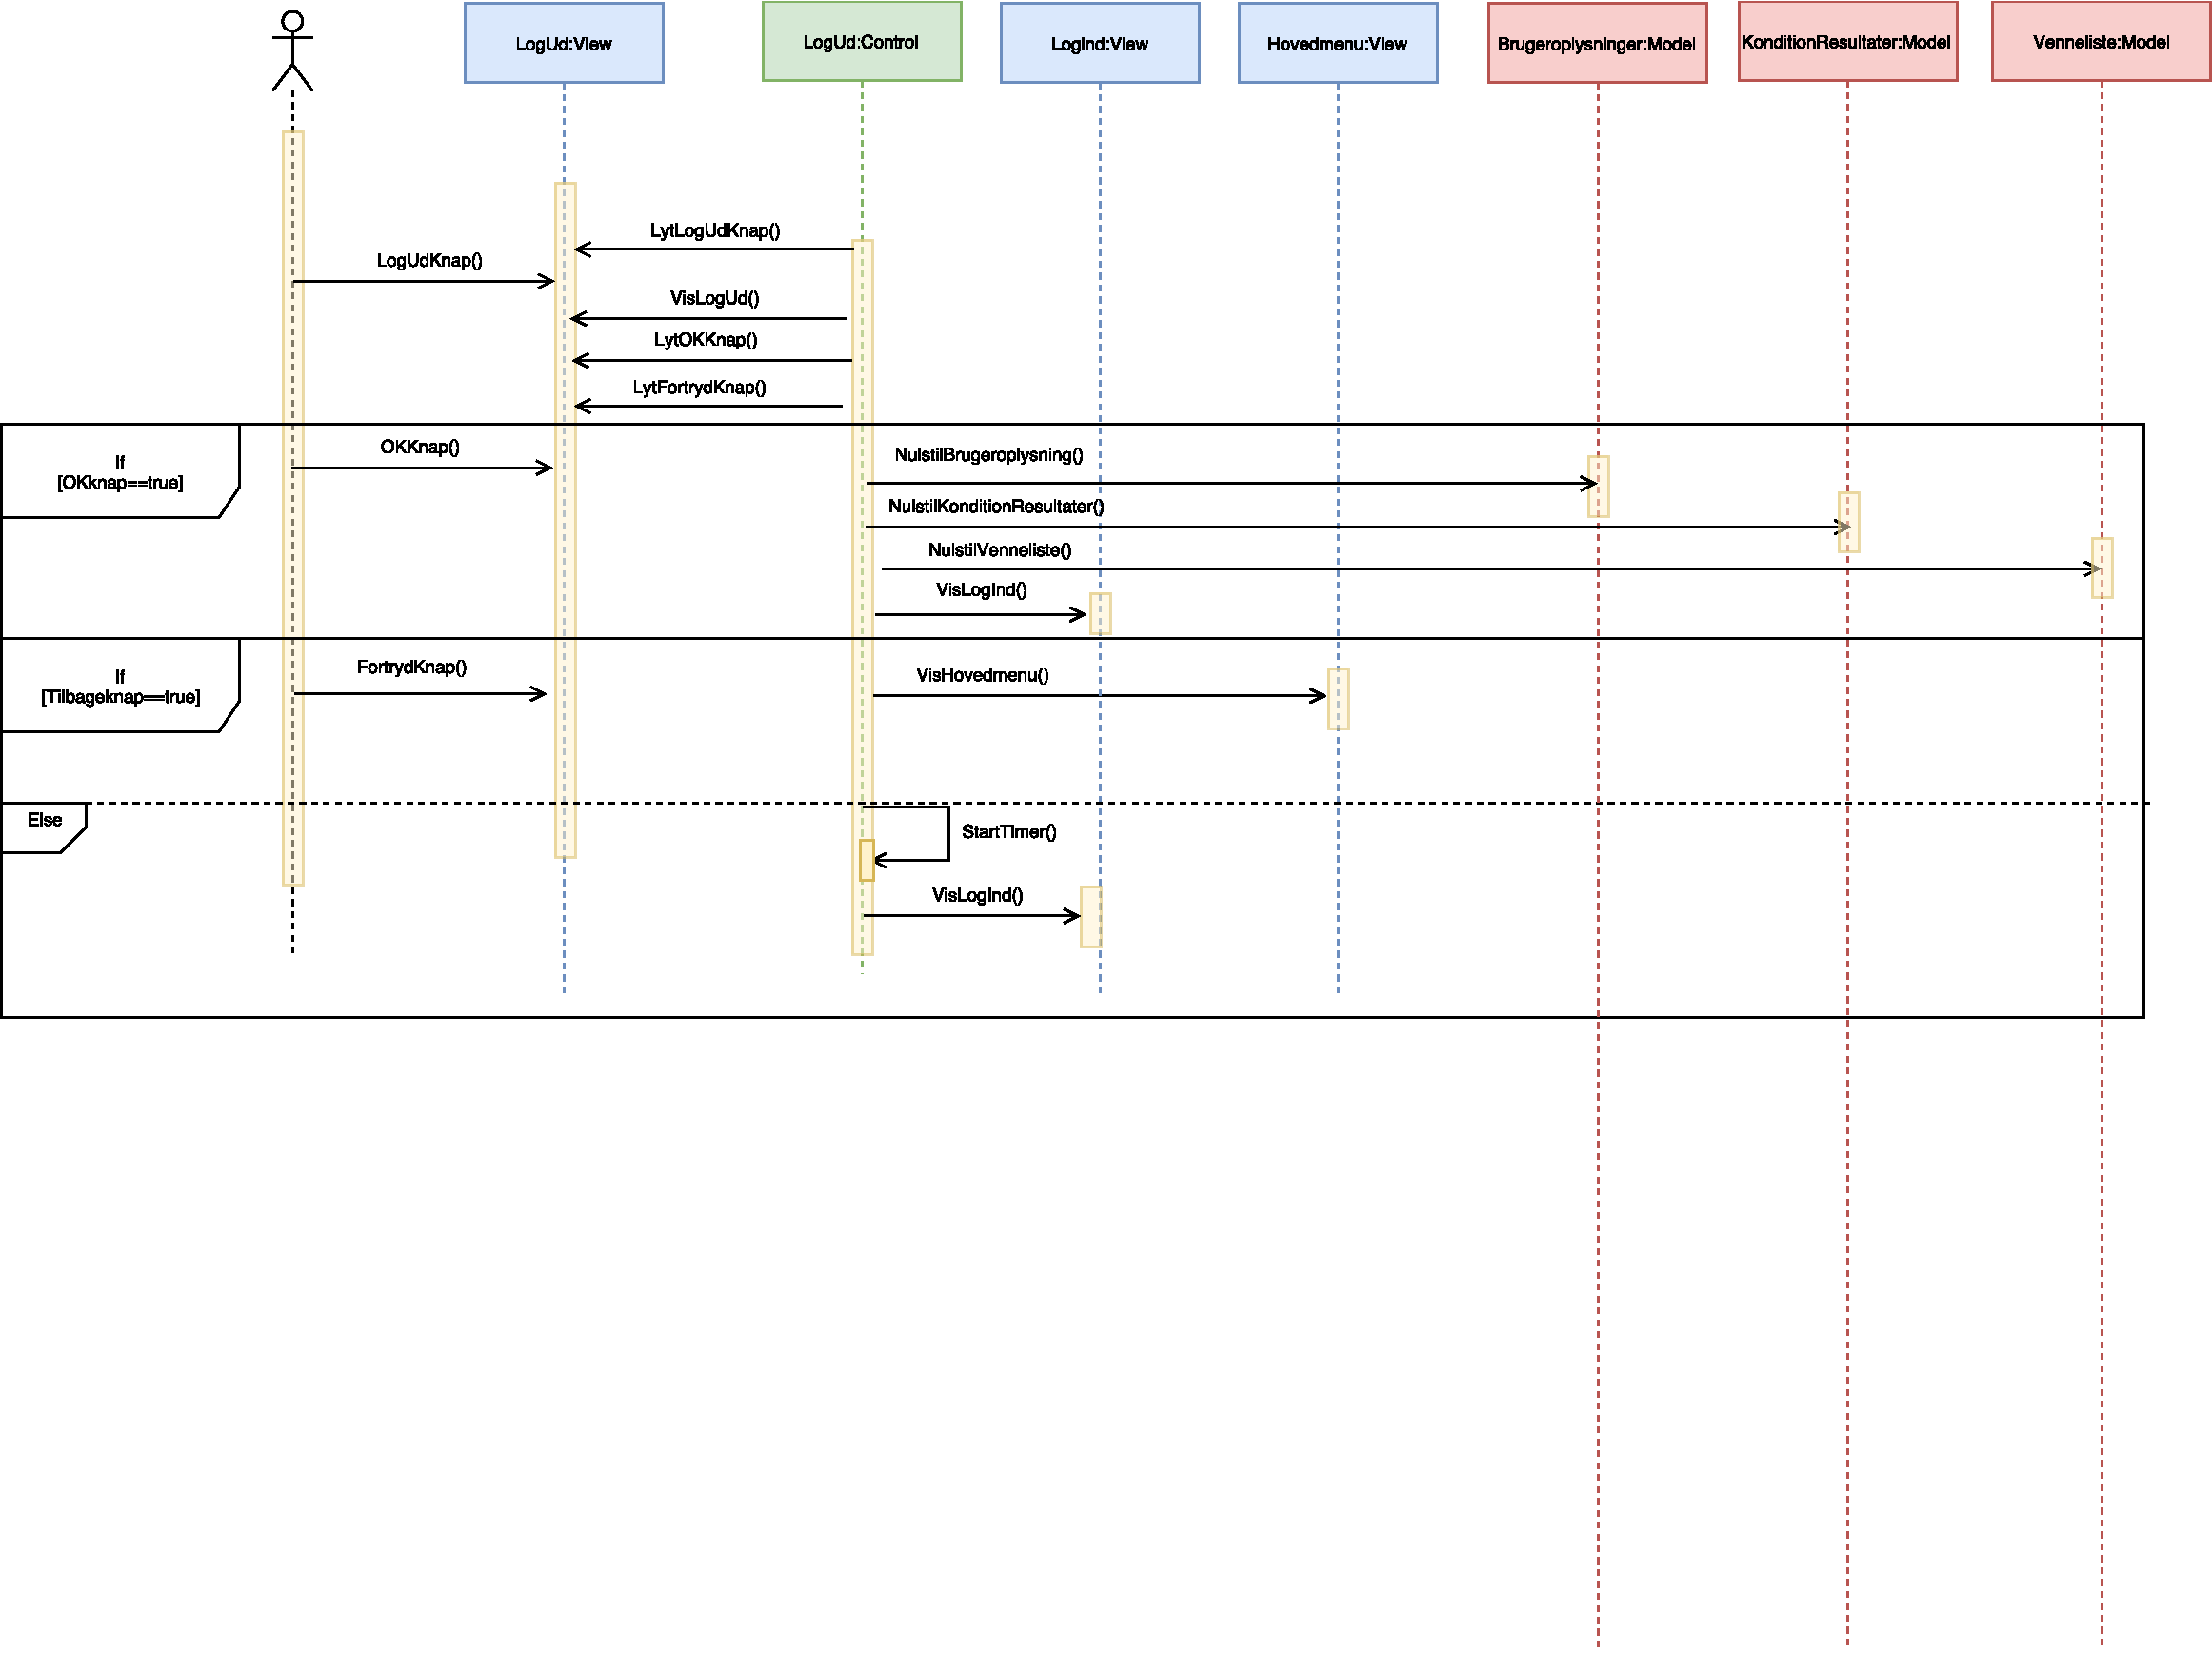
\includegraphics[width=1.28\textwidth]{figures/Sek/SEKLogUd}
\caption{Sekvensdiagram for log ud.}
\label{fig:SEKlogUd}
\end{figure}

\noindent
Når brugeren via grænsefladen for hovedmenuen trykker på knappen for log ud vises grænsefladen for \textit{Log ud}. Her har brugeren mulighed for at trykke på BekræftKnap eller FortrydKnap. Hvis brugeren trykker på BekræftKnap, nulstilles modellen for \textit{Brugeroplysninger} og \textit{Venneliste}, hvorefter grænsefladen for \textit{Log ind} vises. Trykker brugeren på FortrydKnap, vises grænsefladen for \textit{Hovedmenu} igen. 


%% Design af database
\section{Design af database} \label{sec:ER}
Det ønskes, at brugerdata er knyttet til den enkelte bruger i databasen. Dette er med henblik på, at app'en ikke skal lagre større mængder data på den mobile enhed samt sikre data i tilfælde af uforudsete hændelser, som eksempelvis tab af mobil enhed. Databasen skal indeholde oplysninger om de enkelte KOL-patienter, herunder resultater opnået ved træning og vennerelation. 

\subsection{ER-diagram}
Modellering af databasen udarbejdes ud fra et ER-diagram. ER-diagrammet relaterer sig til én KOL-patient i databasen. Databasen tager udgangspunkt i entiteter, som sundhedspersonale, KOL-patient, vennerelation, træning og belønninger. ER-diagrammet for databasen fremgår af \autoref{fig:ERdiagram}.


\begin{figure} [H]
\centering
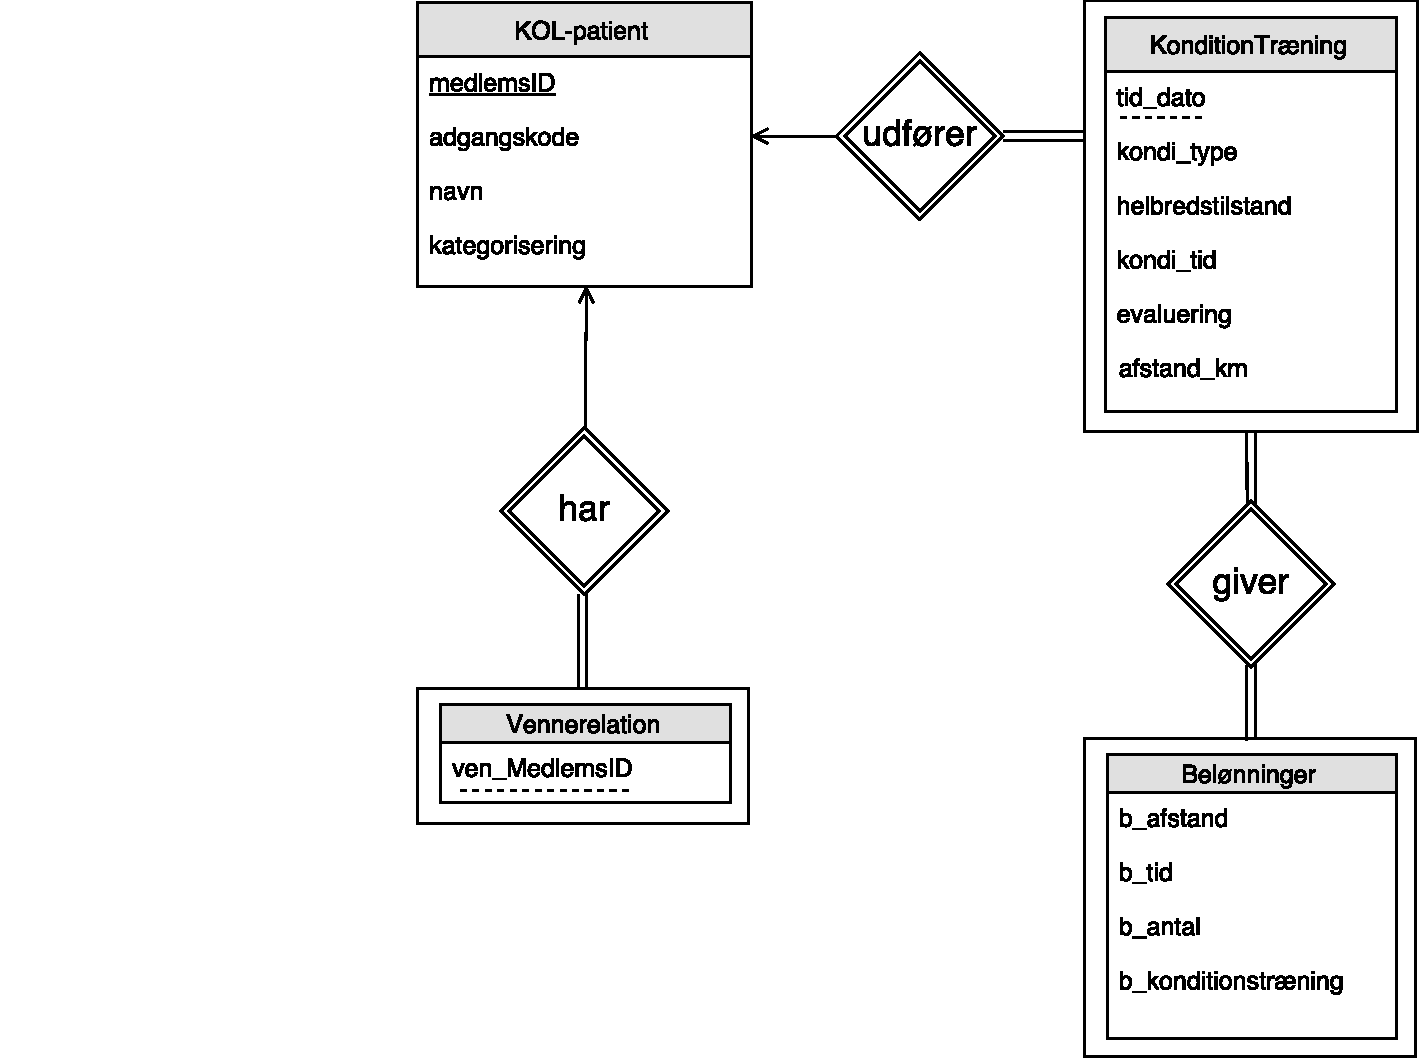
\includegraphics[width=1\textwidth]{figures/Aktivitetsdiagram/ERdiagram}
\caption{ER-diagram for database.}
\label{fig:ERdiagram}
\end{figure} 

\noindent
Af \autoref{fig:ERdiagram} ses ER-diagrammet over databasen, hvori KOL-patienter oprettes og informationer om patienterne samt deres resultater lagres. Sundhedspersonalet fremgår som en stærk entitet, der opretter alle KOL-patienter, hvor én KOL-patient oprettes i databasen én gang. Sundhedspersonalet defineres med et personaleID, afdelingID, personalefornavn og personaleefternavn, hvor \textit{personaleID} er primærnøglen, der kan identificere medarbejderen. Den enkelte KOL-patient er en stærk entitiet, som registreres med primærnøglen, \textit{medlemsID}, samt adgangskode, fornavn, efternavn og kategorisering. Derudover fremgår de svage entiteter, herunder vennerelation, træning og belønninger. Én KOL-patient har mange vennerelationer, som kan identificeres ved KOL-patientens \textit{medlemsID} og \textit{venMedlemsID}. Det samme gør sig gældende for træninger, hvor én KOL-patient kan udføre mange træninger, der identificeres ved  \textit{dato/tid} og \textit{medlemsID}. Ligeledes kan belønninger, som er en mange til mange relation, identificeres ved \textit{data/tid} og \textit{medlemsID}.

\subsection{Schema}
ER-diagrammet omskrives til schema for at kunne normalisere og implementere databasen. Normaliseringen anvendes med henblik på at reducere redundans og inkonsistens. Schema er i anden normalform og fremgår af \autoref{tab:schema}. 

\begin{table} [H]
	\centering
  \begin{tabular}{ | l | p{12cm} |} \hline
     \textbf{Stærke entiteter} & Sundhedspersonale = (\underline{personaleID}, afdelingsID, personaleFornavn, personaleEfternavn)
\newline KOL-patient = (\underline{medlemsID}, adgangskode, fornavn, efternavn, kategorisering) \\ \hline
 	\textbf{Svage entiteter} & Træning = (\underline{medlemsID}, \underline{tid/dato}, træningsform, træningstype, daglig helbredstilstand, tid, afstand, evaluering)
 \newline Vennerelation = (\underline{medlemsID}, \underline{venMedlemsID}, venFornavn, VenEfternavn venBelønninger)
\newline Belønninger = (\underline{medlemsID}, \underline{tid/dato}, afstand, tid, antal, konditionstræning)\\ \hline
    \end{tabular}
    \caption{ER-diagram for databasen omskrevet til schema på anden normalform.}
    \label{tab:schema}
\end{table}


\noindent
Schemaet på anden normalform optimeres til tredje normalform, da det giver bedre muligheder ved implementering af databasen. For at komme på tredje normalform fjernes dimensioner, der ikke har en direkte tilgang til primærnøglen. Tredje normalform ses af \autoref{tab:schema3}.


\begin{table} [H]
	\centering
  \begin{tabular}{ | l | p{12cm} |} \hline
     \textbf{Stærke entiteter} & Sundhedspersonale = (\underline{personaleID}, afdelingsID)
\newline KOL-patient = (\underline{medlemsID}, adgangskode, kategorisering) \\ \hline
 	\textbf{Svage entiteter} & Træning = (\underline{medlemsID}, \underline{tid/dato}, træningsform, træningstype, daglig helbredstilstand, tid, afstand, evaluering)
 \newline Vennerelation = (\underline{medlemsID}, \underline{venMedlemsID},  venBelønninger)
\newline Belønninger = (\underline{medlemsID}, \underline{tid/dato}, afstand, tid, antal, konditionstræning)\\ \hline
    \end{tabular}
    \caption{ER-diagram for databasen omskrevet til schema på tredje normalform.}
    \label{tab:schema3}
\end{table}





%%-----------------------Implementering-------------------------
\chapter{Implementering}
I dette kapitel beskrives implementeringen af app'en, der omhandler transformationen fra design til kode. Det vil beskrives, hvilken platform koden implementeres gennem samt den tilhørende database. Derudover beskrives implementeringen af designklasserne, der opdeles i grænseflader samt model- og controllerklasser. Ydermere vil de centrale elementer i app'en beskrives. Disse elementer omhandler tilpasning af træningsniveau, træning, resultater samt brugerens venneliste. Overordnet vil beskrivelserne tage udgangspunkt i udpluk af den implementerede kode.

I \autoref{cha:design} er analyse- og designklasser samt funktionsnavne navngivet på dansk, hvorfor bogstaverne æ, ø og å forekommer. Disse symboler anvendes ikke under implementeringen. 

Metoderne er tidligere, i \autoref{cha:design}, defineret som private, nogle af disse er dog implementeret som public, da det ønskes at tilgå disse fra andre klasser. 

\section{Platform}
Det er valgt at implementere app'en i platformen Android Studio version 2.3.1 og programmere i Java, da dette er et objektorienteret programmeringssprog \cite{Brahma2015}. Android Studio er et officelt Integrated Development Environment (IDE) for udvikling af android app's \cite{android2017}, hvilket er passende for udviklingenen af dette projekts problemløsning. Dertil tilbyder Android Studio at teste app's på Android Emulator, som kan simulere en android smartphone. Denne kan ses af \autoref{fig:androidEmulator}, hvoraf der til højre for androidskærmen fremgår et kontrolpanel, hvor funktionaliteter for emulatoren kan tilgås. 

\begin{figure} [H]
\centering
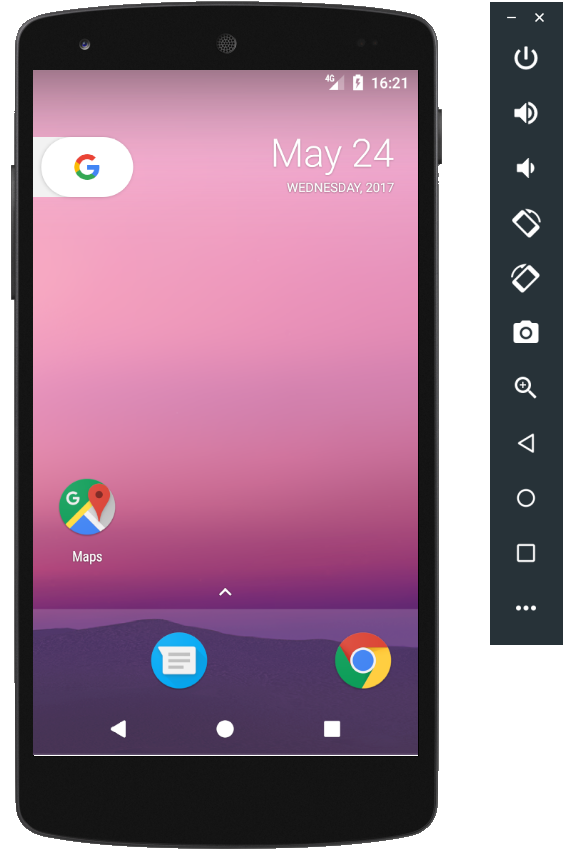
\includegraphics[width=0.5\textwidth]{figures/emulator}
\caption{Android Emulator.}
\label{fig:androidEmulator}
\end{figure}

\noindent
I emulatorens kontrolpanel findes Extended Controls, som fremgår af \autoref{fig:emulatorExtend}. Hertil er det muligt at simulere en android smartphones egenskaber, såsom lokalisation.

\begin{figure} [H]
\centering
\includegraphics[width=1\textwidth]{figures/emulatorExtend}
\caption{Android Emulator.}
\label{fig:emulatorExtend}
\end{figure}

\subsection*{Struktur af Android Studio}
Strukturen i Android Studio opdeles i \textit{manifests}, \textit{res} samt \textit{java} mapper. \textit{Manifests} mappen indeholder en \textit{AndroidManifest.xml} fil, der er essentiel for, at app'en kan køre og indeholder de aktiviter, der implementeres. Derudover er der i denne fil defineret tilladelser for den givne app. For udvikling af app'en har det været nødvendigt at tillade brug af internet samt GPS-lokalisation, for således at kunne tilgå databasen og beregne afstand. 
\textit{Res} mappen indeholder ikke-kode ressourcer, der eksempelvis er de forskellige layouts, som udgør grænsefladerne.
Javaklasserne, der er oprettet i forbindelse med udviklingen af app'en er placeret i \textit{java} mappen.\cite{android2017}
 
\section{Database}
Til implementering af databasen samt kommunikation med denne benyttes programmet XAMPP. Programmet opretter en lokal apache webserver samt database på en given computer, der fungerer som et Localhost miljø. Den lokale webserver simulerer en ekstern webserver, hvilket giver et passende miljø til at teste og udvikle prototypen. Dertil anses dette ikke som værende fjernt fra et virkelighedsnært scenarie, hvor systemet benyttes med ekstern server og database.
Ved direkte håndtering af databasen benyttes phpMyAdmin, der er et online databaseadministrationssystem, som understøtter Structured Query Language (SQL) \cite{silbershatz2011}. 
Databasen er implementeret under navnet \textit{db\_KOL}, hvori tabeller oprettes på baggrund af design jf. \autoref{sec:ER} i relation til attributter og datatyper.

\subsection*{Kommunikation med databasen}
Kommunikation mellem Android Studio og databasen kan ikke forekomme direkte, hvorfor php: Hypertext preprocessor scripts benyttes. Php er et Server-Side Scripting Language, hvilket køres på serveren og muliggør, at systemet kan tilgå databasen \cite{silbershatz2011}. Dertil kan de oprettede php-scripts betragtes som controlleren for database, der er designet i \autoref{sec:databaseDesign}.
Der er oprettet et php-script, \textit{config.php}, der indeholder informationerne host, bruger, adgangskode samt navn på den oprettede database. Dette script inkluderes i et seperat script, \textit{DB\_connect.php}, til at etablere forbindelsen til databasen. Der er opstillet forskellige php-scripts, som javakoden refererer til via URL links. Af disse links fremgår ip-adressen for serveren samt filplaceringen af det givne script. 

De forskellige scripts får information fra app'en for således at kunne udføre SQL-kommandoer. Informationen sendes fra app'en som en JavaScript Object Notation (JSON) repræsentation. JSON benyttes ved dataoverførsel, der gør det muligt at pakke data som et objekt eller array.\cite{silbershatz2011} Php-scripts brugt i dette projekt er sat op til at tjekke, hvorvidt der bliver sendt en værdi i det respektive navn. Er værdierne sat og ikke NULL, ligges værdierne i en ny variabel. Et eksempel af dette ses af \autoref{fig:phplogind}, hvor et udklip af php-scriptet for log ind er visualiseret. 

\begin{figure} [H]
\centering
\includegraphics[width=1\textwidth]{figures/imple/phplogind}
\caption{Udklip af log ind php-script, hvor medlemsid samt adgangskode modtages og indsættes i tilhørende variabler, der benyttes i et funktionskald.}
\label{fig:phplogind}
\end{figure}

\noindent
Dette udklip viser, hvordan koden modtages og gemmes i nye variabler. Værdierne gemmes i et associativt array, der ved hjælp af en POST-metode gør det muligt at overføre data til et andet script, \textit{db\_functions.php}, hvori SQL-kommandoer udføres \cite{w3schools2017}. Linje 21 viser, hvordan variablerne benyttes i et funktionskald, der eksekveres i \textit{db\_functitons.php}. Af \autoref{fig:phplogindsql} ses et udklip af denne funktion.

\begin{figure} [H]
\centering
\includegraphics[width=1\textwidth]{figures/imple/phplogindsql}
\caption{Udklip af php-scripts for funktionen log ind. Herunder ses SQL-kommandoen for denne funktion.}
\label{fig:phplogindsql}
\end{figure}

\noindent
Det ses af \autoref{fig:phplogindsql}, hvordan en SQL-kommando udføres. Tabellen \textit{users} er tidligere i \autoref{sec:ER} defineret KOL-patient. Den viste SQL-kommando henter alt fra tabellen \textit{users} tilhørende medlemsid'et i databasen, der er lig spørgsmåltegn. Spørgsmåltegnet markerer et bindingspunkt, hvorpå en parameter kan tilknyttes. Parameteren, der bindes på ved brug af \textit{bind\_param}, fremgår af linje 176, hvoraf \textit{"s"} indikerer, at medlemsid'et er af typen string. I dette tilfælde valideres log ind-informationerne førend user returneres til log ind php-scriptet, der håndterer user, hvilket fremgår af \autoref{fig:phplogindresp}.


\begin{figure} [H]
\centering
\includegraphics[width=1\textwidth]{figures/imple/phplogindresp}
\caption{Udklip af php-scripts, hvori user håndteres og sendes til app'en.}
\label{fig:phplogindresp}
\end{figure}

\noindent
Som det ses af \autoref{fig:phplogindresp} opstilles if/else statement, der håndterer, hvorvidt \textit{user} returneres. Hvis \textit{user} returneres bliver brugerdata gemt i \textit{response}, der sendes tilbage til app'en som en JSON repræsentation. Returneres \textit{user} ikke, gemmes en fejlmeddelelse i \textit{response}, der ligeledes sendes til app'en som en JSON repræsentation. 

Der er i javakoden opsat en \textit{Response.listener}, der lytter efter respons. Ved respons oprettes et nyt JSON objekt, hvori responset lagres, således dette kan benyttes i app'en. 


\section{Grænseflader}
Til at implemtere grænseflader i systemet benyttes XML-filer, der håndteres i deres respektive controllere. I disse filer er det muligt at definere, hvilken type elementer, der skal indgå i layoutet. Dertil kan typen af layout defineres alt efter, hvordan layoutet skal opstilles. Layouts brugt i dette system er af type linear og relative.  

Elementer, såsom TextView og Button, opstilles i layouts med type, størrelse samt orientering. Forekommer det, at elementerne skal benyttes i javakoden, defineres disse ligeledes med et id. Et eksempel af layoutkode fra log ind ses af \autoref{fig:logindlay}.

\begin{figure} [H]
\centering
\includegraphics[width=0.6\textwidth]{figures/imple/logindlay}
\caption{Udklip af kode fra log ind-layout. Udklippet viser et \textit{EditText}, hvori brugeren angiver adgangskode samt en Button for log ind.}
\label{fig:logindlay}
\end{figure}

\noindent
Af dette udklip ses koden for tekstfeltet, hvori brugeren angiver adgangskode samt koden for layoutet af log ind-knappen. Feltet for adgangskoden er her af typen \textit{EditText}, der tillader, at brugeren kan angive tekst. Dette felt har ligeledes et id, der muliggør at referere til feltet og hente den angivne adgangskode til validering af log ind. Knappen er opstillet af typen \textit{Button} og har ligeledes et id, hvortil en listener er opstillet i javakoden. Dette ses yderligere af \autoref{fig:list}.

\section{Model- og controllerklasser} \label{sec:impmodelcon}
Model- og controllerklasser er implementeret i Java Class-filer. Heri er klasser defineret med navn samt tilhørende attributter og metoder. Af \autoref{fig:javaclass} ses et eksempel på, hvordan en controller er implementeret. 

\begin{figure} [H]
\centering
\includegraphics[width=0.6\textwidth]{figures/imple/javaclass}
\caption{Udpluk af javaklassen for LoginController. Punktummerne symboliserer den resterende kode, der ikke anses nødvendig for forklaring af opsætning af javaklasser.}
\label{fig:javaclass}
\end{figure}

\noindent
Det fremgår af dette udklip, at klassen, \textit{LoginController}, er af typen public og nedarver \textit{activity}. Dette gør sig gældende for samtlige klasser implementeret. Denne klasse for \textit{LoginController} har attributten \textit{btnLogin}, der refererer til log ind-knappen på grænsefladen. Idet app'en skal reagere, når brugeren trykker på log ind-knappen, opsættes en listener på knappen, hvilket ses af \autoref{fig:list}.


\begin{figure} [H]
\centering
\includegraphics[width=0.6\textwidth]{figures/imple/list}
\caption{Udpluk af koden for listeneren opsat for log ind-knappen. Punktummerne symboliserer den resterende kode, der ikke anses nødvendig for forklaring af opsætning af listener.}
\label{fig:list}
\end{figure}


\noindent
Af dette udklip ses den opsatte listener, der har til formål at lytte på knappen. Indenfor listeneren er der opstillet kode, hvilket symboliseres ved punktummer, der køres idet der trykkes på knappen. Denne listener er ligeledes implementeret for samtlige knapper i controllerklasserne, da det er disse filer, som håndterer input for de tilhørende layouts.

Modelklasserne er implementeret på samme vis som controllerklasserne, de har dog til formål at lagre data forinden det sendes til databasen. I disse klasser er der ligeledes opstillet attributter med tilhørende get- og set-metoder. 


\section{Tilpasning af træningsniveau}
I tilpasningscontrolleren beregnes den anbefalede træningstid. Dette gøre ud fra kategorisering, den daglige helbredstilstand og en tidligere evaluering, foretaget efter samme træningsform, -type og helbredstilstand.
Beregningen for den anbefalede træning er implementeret ved brug af if/else-statement. Et udpluk af denne beregning fremgår af \autoref{fig:anbekode}.  
   
\begin{figure} [H]
\centering
\includegraphics[width=1\textwidth]{figures/imple/anbekode}
\caption{Udpluk af koden for anbefalet træning. If/else-loops afgør, hvilket træningsniveau brugeren får anbefalet.}
\label{fig:anbekode}
\end{figure} 

\noindent
Af figuren ses beregningen af den anbefalede træningstid for brugeren med kategorisering \textit{A} og heldbredstilstanden på \textit{2}. Variationen for anbefalingen afhænger af evalueringen og kan i dette eksempel variere mellem \textit{15}, \textit{20} og \textit{25}  minutter. Metodekaldet \textit{setMinutter} referer til, at der sættes en bemærkning, idet den anbefaldede træningstid er opnået.

\section{Træning}
Træningscontrolleren har til formål at håndtere GPS-lokalisation for at beregne tilbagelagt afstand under træning. Ligeledes håndterer controlleren en timer, der viser tiden brugt til den givne træning. Efter træningen er udført, vil træningscontrolleren opsætte en notifikation som efterfølgende vises dagligt. 


\subsection{Afstandsberegning}
For at implementere GPS skal app'en have tilladelse til at anvende den mobile enheds lokalisation. Dette er en engangstilladelse, der skal gives første gang brugeren vil foretage en træning. 

Der instansieres en LocationManager og LocationListener. LocationManager tillader app'en at opnå enhedens lokalisation, hvor LocationListener modtager lokalisationsopdateringer. Disse opdateringer forekommer, idet enheden ændrer lokalisation.\cite{LocationManager, LocationListener} Af koden i \autoref{fig:gpsKode} fremgår det, at systemet indeholder en metode, \textit{onLocationChanged}, der kaldes, når lokalisationen ændres. 

\begin{figure} [H]
\centering
\includegraphics[width=1\textwidth]{figures/imple/gpsKode}
\caption{Metoden, onLocationChanged, der kaldes, når lokalisation ændres.}
\label{fig:gpsKode}
\end{figure} 

\noindent
Når lokalisationen ændres, hentes enhedens longitude og latitude, hvortil disse værdier benyttes i set-metoder. Afstanden beregnes ud fra følgende formel:

\begin{equation} \label{equ:GPS}
d = \arccos(\sin(lat_1)*\sin(lat_2)+\cos(lat_1)*\cos(lat_2)*\cos(lon_2-lon_1))*R
\end{equation}

\noindent
Formlen, der ses af \autoref{equ:GPS}, benyttes til at udregne afstand ud fra to longitude- og latitudepunkter. Af formlen betegner \textit{d} den udregnede afstand, \textit{$lat_1$}, \textit{$lon_1$} samt \textit{$lat_2$}, \textit{$lat_2$} er latitude- og longitudekoordinaterne for henholdsvis den første og anden lokalisation. \textit{R} betegner jordens radius.\cite{Deza2009}    

Ligning \ref{equ:GPS} implementeres i javakode, hvortil denne benytter longitude- og latitudekoordinaterne, der hentes fra koden, som ses af \autoref{fig:gpsKode}. Implementeringen af formlen ses af \autoref{fig:distanceKode}.

\begin{figure} [H]
\centering
\includegraphics[width=1\textwidth]{figures/imple/distanceKode}
\caption{Metode i træningscontrolleren, der beregner afstanden i kilometer ud fra lokalisationer.}
\label{fig:distanceKode}
\end{figure}
 
\noindent
Metoden, \textit{distance}, kaldes hver gang, der sker en lokalisationsændring og beregner afstanden mellem enhedens pågældende lokalisation samt forrige lokalisationsopdatering. Af koden fremgår det, at latitude- og longitudeværdierne konverteres fra grader til radianer for at kunne anvende cosinus- og sinusfunktionerne. 
Afstanden ønskes udregnet i kilometer, hvortil \textit{dist} ganges med jordens radius i kilometer. 
Efterfølgende sættes den udregnede totale afstand \textit{nyDist}, hvortil denne værdi hentes og gemmes i variablen \textit{gammelDist}.   


\subsection{Timer}
I træningscontrolleren startes en timer for at kunne monitorere træning. Denne er implementeret ved at instansiere klassen \textit{Runnable}, hvori en metode, \textit{run}, defineres. Koden for dette kan ses i \autoref{fig:timerKode}.

\begin{figure} [H]
\centering
\includegraphics[width=1\textwidth]{figures/imple/timerKode}
\caption{Udklip af kode fra træningscontrolleren. Udklippet viser metoden for timeren.}
\label{fig:timerKode}
\end{figure} 

\noindent
Metoden, \textit{run}, indeholder variablen \textit{MillisecondTime}, der tæller tiden, som er gået siden brugeren har trykket start træning. Vælger brugeren at trykke stop træning, stopper \textit{MillisecondTime} med at tælle op, hvortil denne værdi gemmes i variablen \textit{TimeBuff}.  Værdien gemmes for, at timeren vil kunne fortsætte, hvis brugeren ønsker at fortsætte træningen. \textit{Seconds} defineres ud fra \textit{UpdateTime}, der måles i millisekunder. Det defineres yderligere, at \textit{Seconds} kun kan tælle op til 60.

Under tilpasning af træningsniveau er der blevet anbefalet en træningstid. Opnår træningstiden denne værdi under træning, vil app'en gøre brugeren opmærksom på dette ved angivelse af en lyd. Dette er implementeret ved en if-loop, hvori klassen MediaPlayer instansieres, hvis den anbefalede tid opnås. Hertil kaldes en metode, der afspiller en lydfil. 


\subsection{Notifikation}
Ifølge de opstillede kravspecifikationer skal app'en sende en daglig notifikation. Denne er implementeret i træningscontrolleren, hvor notifikationen aktiveres første gang brugeren har evalueret en træning. Hertil er det implementeret, ved brug af klassen \textit{Calendar} og metoderne \textit{getInstance}, at den daglige notifikation sendes klokken 15. Af \autoref{fig:notifikationKode} fremgår et udklip af koden, som definerer tidspunktet for notifikationen. 

\begin{figure} [H]
\centering
\includegraphics[width=0.8\textwidth]{figures/imple/notifikationKode}
\caption{Udklip af kode fra træningscontrolleren, som viser notifikationens starttidspunkt.}
\label{fig:notifikationKode}
\end{figure} 

\section{Resultater}
For at brugeren kan følge sin egen udvikling er der implementeret et BarChart. Denne graf viser tiden, brugeren har trænet for den givne uge. Af denne graf plottes en træningstid for hver af ugens dage. Af \autoref{fig:koderesul} fremgår et udpluk af implementeringen for den opstillede graf.

\begin{figure} [H]
\centering
\includegraphics[width=0.9\textwidth]{figures/imple/koderesul}
\caption{Udklip af javakode for BarChart, der senere har til formål at illustrere brugerens ugentlige træningstid.}
\label{fig:koderesul}
\end{figure} 

\noindent
Der ses af dette udklip, at der oprettes et ArrayList under navnet \textit{barEntries}. Dette array anvendes til at lagre mængden af data, der ønskes plottet. Dertil ses det, hvorledes nye elementer tilføjes dette array ud fra en værdi og index. Værdien, der instættes tages fra et andet array af navnet \textit{data}, hvori der lagres en træningstid for ugens dage. Plads nummer \textit{0} refererer til den første dag i ugen og tæller således op efter ugens dage. \textit{Data} er divideret med 60, da træningstiden er gemt som sekunder og ønskes plottet i minutter. 

Belønninger gives udfra samlet tid, afstand, antal træninger samt antal konditionstræninger og beregnes efter endt træning. Da disse belønninger er baseret ud fra den samlede træning, hentes den sammenlagte tid, afstand samt totale antal træninger fra databasen og omregnes til et tal mellem 1 til 6, der repræsenterer antallet af stjerner brugeren har opnået. Et udklip af javakoden for omregningen for brugere med en kategorisering \textit{A} ses af \autoref{fig:kodebelon}.

\begin{figure} [H]
\centering
\includegraphics[width=0.8\textwidth]{figures/imple/kodebelon}
\caption{Udklip af javakode for omregning af samlet afstand til optjente belønninger for brugere med kategorisering \textit{A}.}
\label{fig:kodebelon}
\end{figure} 

\noindent
Det fremgår af dette javaudklip, at omregningen foregår ved if/else-loops. Hvis afstanden ligger indenfor et interval af 5 og 25, sættes \textit{b\_afstand} lig 1, hvilket repræsenterer én stjerne. Af \autoref{tab:SamletBelon} fremgår kriterierne for at opnå stjerner for brugere med kategoriseringen \textit{A}.  

\begin{table}[H]
\centering
\includegraphics[width=0.8\textwidth]{figures/imple/SamletBelon}
\caption{Kriterier for at opnå belønninger inden for henholdsvis samlet tid, afstand og total antal træninger samt konditionstræninger for brugere med kategorisering \textit{A}.}
\label{tab:SamletBelon}
\end{table}  

\section{Venneliste}
I vennelistecontrolleren er der implementeret en venneliste, som indeholder brugere, der følges. For at app'en kan hente venner som brugeren følger, sendes brugerens medlemsID til databasen. Et php-script benytter medlemsID i en SQL-kommando, der tilgår tabellen for vennerelationer, som returnerer ven_mendlemsid for de brugere, der følges. 
Dette modtages i app'en som et JSON-objekt, hvorfra et JSON-array hentes og ligges i venner_array, der kan ses af udklippet i  \autoref{fig:vennerKode}.  

\begin{figure} [H]
\centering
\includegraphics[width=1\textwidth]{figures/imple/vennerKode}
\caption{Udpluk af koden for venneliste. Koden viser et udpluk af, hvordan venners navn og medlemsID gemmes i arraylisten, VenneListe.}
\label{fig:vennerKode}
\end{figure} 

Af koden i figuren er der opsat en for-loop hvori JSON objekter hentes fra alle palceringerne i venner_array. Hvert af disse objekter repræsentere en af brugerens venner, hvor værdier for navn og ven_medlemsid hentes for disse. 
Af for-loopen ses det, at objekterne gemmes i et nyt array af navnet VenneListe, som senere benyttes til at vise vennerne i ListView for grænsefladen. Grundet bruget af HashMap til at håndtere navn og medlemsID, har det været nødvendigt at håndtere medlemsID som en string. Dette skyldes, at ved instansiering af Hashmappet defineres indputtyperne som string, idet navnet kun kan være af typen string. 

Der er i app'en mulighed for at tilføje og fjerne brugere fra vennelisten. Muligheden for at tilføje en bruger til vennelisten er implementeret ved at benytte SQL-kommandoen, der ses af \autoref{fig:opretVenKode}.

\begin{figure} [H]
\centering
\includegraphics[width=1\textwidth]{figures/imple/opretVenKode}
\caption{SQL-kommando for tilføj bruger til venneliste.}
\label{fig:opretVenKode}
\end{figure}

I ovenstående kode ses det, at medlemsid og ven_medlemsid indsættes i tabellen Vennerelation, hvorved der dannes en vennerelation. Fjernes en bruger fra vennelisten, anvendes SQL-kommandoen, der fremgår af \autoref{fig:fjernVenKode}. Dertil er forskellen fra at oprette en vennerelation, at SQL-kommandoen anvender delete, og dermed fjerner vennerelationen fra tabellen i databasen. Hertil fjernes relationen kun der, hvor både medlemsID for bruger og ven indgår. 

\begin{figure} [H]
\centering
\includegraphics[width=1\textwidth]{figures/imple/fjernVenKode}
\caption{SQL-kommando for fjern bruger til venneliste.}
\label{fig:fjernVenKode}
\end{figure}


%\subsection{Implementering af objektorienteret design}
I afsnittet vil der fremgå udsnit af Java kode og i nogle tilfælde figurer af grænseflader. Dette er valgt, da nogle funktioner er kompliceret at beskrive. 

\subsubsection*{Log ind}
%\section{Database}
Til implementering af databasen samt kommunikation med denne benyttes programmet XAMPP. Programmet opretter en lokal apache webserver samt database på en given computer, der fungerer som et Localhost miljø. Den lokale webserver simulerer en ekstern webserver, hvilket giver et passende miljø til at teste og udvikle prototypen. Dertil anses dette ikke som værende fjernt fra et virkelighedsnært scenarie, hvor systemet benyttes med ekstern server og database.
Ved direkte håndtering af databasen benyttes phpMyAdmin, der er et online databaseadministrationssystem, som understøtter Structured Query Language (SQL) \cite{silbershatz2011}. 
Databasen er implementeret under navnet \textit{db\_KOL}, hvori tabeller oprettes på baggrund af design jf. \autoref{sec:ER} i relation til attributter og datatyper.

\subsection{Kommunikation med databasen}
*********** DB controller = PHP script!***********
Kommunikation mellem Android Studio og databasen kan ikke forekomme direkte, hvorfor php: Hypertext preprocessor scripts benyttes. Php er et Server-Side Scripting Language, hvilket køres på serveren og muliggør, at systemet kan tilgå databasen \cite{silbershatz2011}. 
Der er oprettet et php-script, \textit{config.php}, der indeholder informationerne host, bruger, adgangskode samt navn på den oprettede database. Dette script inkluderes i et seperat script, \textit{DB\_connect.php}, til at etablere forbindelsen til databasen. Der er opstillet forskellige php-scripts, som javakoden refererer til via URL links. Af disse links fremgår ip-adressen for serveren samt filplaceringen af det givne script. 

De forskellige scripts får information fra app'en for således at kunne udføre SQL-kommandoer. Informationen sendes fra app'en som en JavaScript Object Notation (JSON) repræsentation. JSON benyttes ved dataoverførsel, det er hertil muligt at pakke data som et objekt eller array.\cite{silbershatz2011} Php-scripts brugt i dette projekt er sat op til at tjekke, hvorvidt der bliver sendt en værdi i det respektive navn. Er værdierne sat og ikke NULL, ligges værdierne i en ny variabel. Et eksempel af dette ses af \autoref{fig:phplogind}, hvor et udklip af php-scriptet for log ind er visualiseret. 

\begin{figure} [H]
\centering
\includegraphics[width=1\textwidth]{figures/imple/phplogind}
\caption{Udklip af log ind php-script, hvor medlemsid samt adgangskode modtages og indsættes i tilhørende variabler, der benyttes i et funktionskald.}
\label{fig:phplogind}
\end{figure}

\noindent
Dette udklip viser, hvordan koden modtages og gemmes i nye variabler. Værdierne gemmes i et associativt array, der ved hjælp af en POST-metode gør det muligt at overføre data til et andet script, \textit{db\_functions.php}, hvori SQL-kommandoer udføres \cite{w3schools2017}. Linje 21 viser, hvordan variablerne benyttes i et funktionskald, der eksekveres i \textit{db\_functitons.php}. Af \autoref{fig:phplogindsql} ses et udklip af denne funktion.

\begin{figure} [H]
\centering
\includegraphics[width=1\textwidth]{figures/imple/phplogindsql}
\caption{Udklip af php-scripts for funktionen log ind. Herunder ses SQL-kommandoen for denne funktion.}
\label{fig:phplogindsql}
\end{figure}

\noindent
Det ses af \autoref{fig:phplogindsql}, hvordan en SQL-kommando udføres. Den viste SQL-kommando henter alt fra tabellen \textit{users} tilhørende medlemsid'et i databasen, der er lig spørgsmåltegn. Spørgsmåltegnet markerer et bindingspunkt, hvorpå en parametre kan tilknyttes. Parameteren, der bindes på ved brug af \textit{bind\_param}, fremgår af linje 176, hvoraf \textit{"s"} indikerer, at medlemsid'et er af typen string. I dette tilfælde valideres log ind-informationerne førend user returneres til log ind php-scriptet, der håndterer user, hvilket fremgår af \autoref{fig:phplogindresp}.


\begin{figure} [H]
\centering
\includegraphics[width=1\textwidth]{figures/imple/phplogindresp}
\caption{Udklip af php-scripts, hvori user håndteres og sendes til app'en.}
\label{fig:phplogindresp}
\end{figure}

\noindent
Som det ses af \autoref{fig:phplogindresp} opstilles if/else statement, der håndterer, hvorvidt \textit{user} returneres. Hvis \textit{user} returneres bliver brugerdata gemt i \textit{response}, der sendes tilbage til app'en som en JSON repræsentation. Returneres \textit{user} ikke, gemmes en fejlmeddelelse i \textit{response}, der ligeledes sendes til app'en som en JSON repræsentation. 

Der er i javakoden opsat en \textit{Response.listener}, der lytter efter respons. Ved respons oprettes et nyt JSON objekt, hvori responset lagres, således dette kan benyttes i app'en. 
%%-----------------------Test-------------------------%%
\chapter{Test}
I dette kapitel beskrives test af app'en. Der tages udgangspunkt i at teste kravspecifikationer der blev opstillet i \autoref{sec:funktionellekrav}, hvorefter der blev opstillet et use casediagram på baggrund af disse. Testene er opdelt i database og de forskellige use cases. Hver test vil indeholde navnet på testen samt en beskrivelse af formålet og main flowet for testen. Efter hvert main flow beskrives det forventede output, hvorefter det samlede resultat af testen vil fremgå af resultat.  

\section{Database}
Databasen anvendes i forbindelse med registrering af brugere. Derudover skal det være muligt for systemet at hente og gemme data i en database. Der blev opstillet følgende funktionelle krav til database:
 
\begin{itemize}
\item Brugere skal kunne oprettes i en database
\\
\textit{Dette er nødvendigt for, at brugere kan anvende app’en}
\item Systemet skal kunne gemme og hente data i en database
\\
\textit{Dette er nødvendigt for, at brugere kan tilgå brugerdata}
\end{itemize}

\noindent
For at teste om de opstillede krav til databasen er overholdt, udføres testen, som fremgår af \autoref{tab:testDatabase}.

  \begin{longtable}{ | l | p{13cm} |} \hline
    \textbf{Test:} & Database \\ \hline
     \textbf{Formål:} & Formålet er at oprette brugere i databasen samt hente og sende data. Dette gøres ved at oprette en bruger i databasen. Efterfølgende vil en kategorisering foretages, og derefter tjekkes om denne er gemt i databasen. Til sidst skal brugeren gå til rediger adgangskode og tjekke om kategoriseringen er angivet og derved hentet fra databasen. \\ \hline
 	\textbf{Main flow:} & 1.~ Indtast SQL-forespørgsel \textit{INSERT INTO 'users' ('navn', 'medlemsid', 'db\_adgangskode', 'kategorisering') VALUES ('Jens Jensen', '11170301', 'adgangskode', 'F')} i databasen.
 	\begin{itemize}
	\item Bruger er oprettet i databasen 
	\end{itemize}
 2.~Åben app’en og log ind med medlemsID, \textit{11170301}, og adgangskode, \textit{adgangskode}. Udfør kategorisering og få en samlet CAT-score under 10 ved at vælge værdierne \textit{0,1,2,1,0,1,0,1}, tryk videre efter hver angivet værdi. Herefter vælges antallet af indlæggelser til \textit{0 INDLÆGGELSER}. 
 \begin{itemize}
 \item Kategorisering A er gemt i databasen (\textbf{\textit{Figur 1 og 2}})
 \end{itemize}
3.~Tryk på \textit{REDIGER ADGANGSKODE} via hovedmenuen.
\begin{itemize}
\item MedlemsID og navn samt opdaterede kategorisering, A, vises under rediger adgangskode (\textbf{\textit{Figur 3}})
\end{itemize}
 \\  \hline
  \textbf{Resultat:} &
  \hspace{1.5mm}
 \raisebox{-\totalheight}{\includegraphics[width=0.24\textwidth, height=60mm]{figures/test/testdatabase}}
  \hspace{5mm}
   \raisebox{-\totalheight}{\includegraphics[width=0.24\textwidth, height=60mm]{figures/test/testdatabase1}} 
     \hspace{5mm}
    \raisebox{-\totalheight}{\includegraphics[width=0.24\textwidth, height=60mm]{figures/test/testdatabase2}} 
    \vspace{3mm}
    ~~~~~~~~~~~ \textbf{\textit{Figur 1}}~~~~~~~~~~~~~~~~~~~~~~~~\textbf{\textit{Figur 2}}~~~~~~~~~~~~~~~~~~~~~~~~\textbf{\textit{Figur 3}}
    \newline
Resultater for test af database fremgår af ovenstående figurer. Til venstre er der opnået en kategorisering svarende til A, som på figuren i midten viser, at kategoriseringen er gemt i databasen. Til højre vises redigering af adgangskode, hvor brugeroplysninger om den oprettede bruger, Jens Jensen, vises. Disse værdier er hentet fra databasen, idet brugeren logger ind. Dertil er kategoriseringen opdateret i forhold til den nye kategorisering. 
\begin{itemize}[label={\checkmark}]
 \item På baggrund af denne test er kravene for databasen opfyldt
 \end{itemize}
  \\ \hline
    \caption{Test af database.}
    \label{tab:testDatabase}
\end{longtable}


\section{Log ind}
Log ind anvendes for at adskille brugere, som er registreret i databasen. Derudover er det med til at sikre, at brugeren har deltaget i et rehabiliteringsforløb, da det kun er disse brugere, der bliver registreret i databasen. Der er opstillet et funktionelt krav til log ind:

\begin{itemize}
\item Brugere skal kunne logge ind med et personligt medlemsID og adgangskode
\\
\textit{Dette er nødvendigt for at tilgå og sikre, at brugere har deltaget i et rehabiliteringsforløb samt adskille brugeres data}
\end{itemize}

\noindent
Til at teste, hvorvidt kravene til log ind er opfyldt, udføres testen, der fremgår af \autoref{tab:testLogInd}.

  \begin{longtable}{ | l | p{13cm} |} \hline
    \textbf{Test:} & Log ind \\ \hline
     \textbf{Formål:} & Formålet er at teste, hvorvidt log ind-funktionen i systemet opfylder krav opstillet til log ind. Dette gøres ved at logge ind med en bruger, der findes i databasen og en bruger, som ikke findes i databasen. 
 \\ \hline
 	\textbf{Main flow:} & 1.~Indtast et medlemsID, som ikke eksisterer i databasen \textit{123456} og en adgangskode, som eksisterer i databasen \textit{adgangskode} og tryk på log ind knappen.
 	\begin{itemize}
 	\item Log ind mislykkedes. Fejlmeddelelse vises i grænsefladen for log ind (\textbf{\textit{Figur 1}})
 	\end{itemize}
2.~Indtast et MedlemsID, som eksisterer i databasen \textit{11170301} og en adgangskode, som ikke tilhører medlemsID’et \textit{forkertadgangskode} og tryk på log ind-knappen.
 \begin{itemize}
 \item Log ind mislykkedes. Fejlmeddelelse vises i grænsefladen for log ind (\textbf{\textit{Figur 2}})
 \end{itemize}
3.~Indtast et medlemsID \textit{11170301} og en adgangskode \textit{adgangskode}, som eksisterer i databasen. 
\begin{itemize}
\item Log ind lykkedes og hovedmenu vises (\textbf{\textit{Figur 3}})
\end{itemize}
 \\  \hline
 \textbf{Resultat:} &  \hspace{1.5mm}
  \raisebox{-\totalheight}{\includegraphics[width=0.24\textwidth, height=60mm]{figures/test/testlogind1}} 
  \hspace{5mm}
   \raisebox{-\totalheight}{\includegraphics[width=0.24\textwidth, height=60mm]{figures/test/testlogind}} 
     \hspace{5mm}
    \raisebox{-\totalheight}{\includegraphics[width=0.24\textwidth, height=60mm]{figures/test/testlogind2}} 
    \vspace{3mm}
       ~~~~~~~~~~~ \textbf{\textit{Figur 1}}~~~~~~~~~~~~~~~~~~~~~~~~\textbf{\textit{Figur 2}}~~~~~~~~~~~~~~~~~~~~~~~~\textbf{\textit{Figur 3}}
    \newline
Resultater for test af log ind fremgår af ovenstående figurer. Til venstre og i midten testes der for henholdsvis første og andet main flow. Hertil fremgår det, at log ind mislykkedes, hvoraf fejlmeddelelsen vises. Til højre fremgår det, at log ind lykkedes, og hovedmenuen vises.  
\begin{itemize}[label={\checkmark}]
 \item På baggrund af denne test er kravet for log ind opfyldt
 \end{itemize}
 \\ \hline
    \caption{Test af Log ind.}
    \label{tab:testLogInd}
\end{longtable}

\section{Kategorisering}
Kategoriseringen skal foretages første gang brugeren logger ind i app'en og skal være en parameter i tilpasningen af et træningsniveau for den enkelte bruger. Følgende krav blev opstillet til kategoriseringen:

\begin{itemize}
\item Systemet skal kunne kategorisere brugere i ABCD på baggrund af CAT-score og antallet af årlige indlæggelser på grund af KOL
\\
\textit{Dette er nødvendigt for at kunne tilpasse træningen efter den enkelte bruger}
\end{itemize}

\noindent
Det testes, om de opstillede krav til kategorisering er overholdt. Testen fremgår af \autoref{tab:testKategorisering}.

  \begin{longtable}{ | l | p{13cm} |} \hline
    \textbf{Test:} & Kategorisering  \\ \hline
     \textbf{Formål:} & Formålet er, at systemet skal kunne kategorisere brugere i ABCD efter, at  brugeren har svaret på udsagn fra CAT-score og angivet antallet af indlæggelser forårsaget af KOL inden for det seneste år. Dette gøres ved at angive forskellige værdier, der giver kategorisering A, B, C, eller D.
 \\ \hline
 	\textbf{Main flow:} & 1.~Få en samlet CAT-score under 10. Vælg \textit{0,1,2,1,0,1,0,1}, tryk videre efter hver angivet værdi og vælg til sidst antal indlæggelser \textit{0 INDLÆGGELSER} (\textbf{\textit{Figur 1, 2 og 3}}). 
 	\begin{itemize} 
 	\item Kategorisering er A (\textbf{\textit{Figur 4}})
 	\end{itemize}	
 	2.~Få en samlet CAT-score over 10. Vælg \textit{5,1,2,3,4,5,1,5}, tryk videre efter hver angivet værdi og vælg til sidst antal indlæggelser \textit{0 INDLÆGGELSER}.
 	\begin{itemize}
 	\item Kategorisering er B (\textbf{\textit{Figur 5}})
 	\end{itemize}
3.~Få en samlet CAT-score under 10. Vælg \textit{0,1,2,1,0,1,0,1}, tryk videre efter hver angivet værdi og vælg til sidst antal indlæggelser \textit{1 ELLER FLERE INDLÆGGELSER}.
 \begin{itemize}
  \item Kategorisering er C (\textbf{\textit{Figur 6}})
  \end{itemize}
4.~Få en samlet CAT-score over 10. Vælg \textit{5,1,2,3,4,5,1,5}, tryk videre efter hver angivet værdi og vælg til sidst antal indlæggelser \textit{1 ELLER FLERE INDLÆGGELSER}.
\begin{itemize}
\item Kategorisering er D (\textbf{\textit{Figur 7}})
\end{itemize}   \\ \hline
 \textbf{Resultat:} &\hspace{1.5mm}
  \raisebox{-\totalheight}{\includegraphics[width=0.24\textwidth, height=60mm]{figures/test/KAT}} 
  \hspace{5mm}
   \raisebox{-\totalheight}{\includegraphics[width=0.24\textwidth, height=60mm]{figures/test/KAT1}} 
     \hspace{5mm}
    \raisebox{-\totalheight}{\includegraphics[width=0.24\textwidth, height=60mm]{figures/test/KAT2}} 
    \vspace{3mm}
          ~~~~~~~~~~~ \textbf{\textit{Figur 1}}~~~~~~~~~~~~~~~~~~~~~~~~\textbf{\textit{Figur 2}}~~~~~~~~~~~~~~~~~~~~~~~~\textbf{\textit{Figur 3}}
           \newline
Ovenstående figurer viser grænsefladerne for introduktion til kategorisering, CAT-score og antal indlæggelser. Den midterste figur viser et af de otte udsagn, der udgør CAT-scoren. Disse grænseflader vises før grænsefladen for kategorisering.   
 \\ \hline
\textbf{} & \hspace{0.3mm}
  \raisebox{-\totalheight}{\includegraphics[width=0.20\textwidth, height=60mm]{figures/test/testkat1}} 
   \raisebox{-\totalheight}{\includegraphics[width=0.20\textwidth, height=60mm]{figures/test/testkat2}} 
    \raisebox{-\totalheight}{\includegraphics[width=0.20\textwidth, height=60mm]{figures/test/testkat}} 
 \raisebox{-\totalheight}{\includegraphics[width=0.20\textwidth, height=60mm]{figures/test/testkat3}} 
    \vspace{3mm}
               ~~~~~~~~\textbf{\textit{Figur 4}}~~~~~~~~~~~~~~\textbf{\textit{Figur 5}}~~~~~~~~~~~~~~\textbf{\textit{Figur 6}}~~~~~~~~~~~~~~~\textbf{\textit{Figur 7}}
    \newline
Resultater for test af kategorisering fremgår af ovenstående figurer. Fra venstre mod højre ses, at henholdsvis første til fjerde main flow viser de forventede kategoriseringer.
 \begin{itemize}[label={\checkmark}]
\item På baggrund af denne test er kravet for kategorisering opfyldt
\end{itemize} 
\\ \hline
   \caption{Test af kategorisering.}
    \label{tab:testKategorisering}
\end{longtable}

\section{Tilpasning af træningsniveau}
I tilpasning af træningsniveau skal brugeren oplyses et anbefalet træningsniveau, med henblik på at tage højde for daglige variationer, ved at anvende parametrene kategorisering, daglig helbredstilstand og eventuel tidligere evaluering. Følgende krav blev opstillet til tilpasning af træningsnivauet:

\begin{itemize}
\item Brugere skal kunne angive deres daglige helbredstilstand
\\
\textit{Dette er nødvendigt for tage højde for daglige variationer og derved tilpasse træningen for den enkelte bruger}
\end{itemize}

\noindent
Da der blev afgrænset til konditionstræning er testen kun udført med konditionstræning. Derudover er testen opdelt i tilpasning af træningsniveau med og uden evaluering, da der ved første anvendelse ikke eksisterer en evaluering. Testen for tilpasning af træningsniveau uden evaluering fremgår af \autoref{tab:testTilpasningudenevaluering} og med evaluering af \autoref{tab:testTilpasningmedevaluering}.

  \begin{longtable}{ | l | p{13cm} |} \hline
    \textbf{Test:} & Tilpasning af træningsniveau uden evaluering \\ \hline
     \textbf{Formål:} & Formålet er, at brugeren skal kunne angive ønsket træningsform, træningstype samt daglig helbredstilstand, hvorefter systemet, på baggrund af dette samt brugerens kategorisering, anbefaler et træningsniveau. Dette gøres ved at angive samme træningsform, og vælge mellem de tre forskellige træningstyper og helbredstilsande. Brugeren er i kategoriseringen A.
 \\ \hline
 	\textbf{Main flow:} &
 	1.~Vælg \textit{TRÆNING}, \textit{KONDITIONSTRÆNING}, \textit{LØB}, \textit{MEGET DÅRLIGT} og tryk videre efter hver handling (\textbf{\textit{Figur 1, 2 og 3}}).
 	\begin{itemize}
 	\item Anbefaling af træningstid er 10 min (\textbf{\textit{Figur 4}})
 	\end{itemize}
 	 2~Vælg \textit{TRÆNING}, \textit{KONDITIONSTRÆNING}, \textit{GÅ}, \textit{MODERAT} og tryk videre efter hver handling.
 	\begin{itemize}
 	\item Anbefaling af træningstid er 30 min (\textbf{\textit{Figur 5}})
 	\end{itemize}	
3.~Vælg \textit{TRÆNING}, \textit{KONDITIONSTRÆNING}, \textit{CYKEL}, \textit{MEGET GODT} og tryk videre efter hver handling.
 \begin{itemize}
  \item Anbefaling af træningstid er 50 min (\textbf{\textit{Figur 6}})
  \end{itemize}
 \\  \hline
 \textbf{Resultat:} &\hspace{1.5mm}
  \raisebox{-\totalheight}{\includegraphics[width=0.24\textwidth, height=60mm]{figures/test/tilpasningny}} 
  \hspace{5mm}
   \raisebox{-\totalheight}{\includegraphics[width=0.24\textwidth, height=60mm]{figures/test/tilpasningny1}} 
  \hspace{5mm}
   \raisebox{-\totalheight}{\includegraphics[width=0.24\textwidth, height=60mm]{figures/test/tilpasningny2}} 
\vspace{3mm}
        ~~~~~~~~~~~ \textbf{\textit{Figur 1}}~~~~~~~~~~~~~~~~~~~~~~~~\textbf{\textit{Figur 2}}~~~~~~~~~~~~~~~~~~~~~~~~\textbf{\textit{Figur 3}}
    \newline
Ovenstående figurer viser grænsefladerne for valg af træningsform, træningstype og daglig helbredstilstand. Disse grænseflader vises før grænsefladen for anbefalet træningstid. 
   \\ \hline
  \textbf{} &\hspace{1.5mm}
  \raisebox{-\totalheight}{\includegraphics[width=0.24\textwidth, height=60mm]{figures/test/tilpasning1}} 
  \hspace{5mm}
   \raisebox{-\totalheight}{\includegraphics[width=0.24\textwidth, height=60mm]{figures/test/tilpasning}} 
     \hspace{5mm}
    \raisebox{-\totalheight}{\includegraphics[width=0.24\textwidth, height=60mm]{figures/test/tilpasning2}} 
    \vspace{3mm}
        ~~~~~~~~~~~ \textbf{\textit{Figur 4}}~~~~~~~~~~~~~~~~~~~~~~~~\textbf{\textit{Figur 5}}~~~~~~~~~~~~~~~~~~~~~~~~\textbf{\textit{Figur 6}}
    \newline
    Resultater for test af tilpasning af træningsniveau uden evaluering fremgår af ovenstående figurer. Fra venstre mod højre ses, at henholdsvis første til tredje main flow viser de forventede anbefalinger af træningstider. 
 \\ \hline
   \caption{Test af tilpasning af træningsniveau uden evaluering.}
    \label{tab:testTilpasningudenevaluering}
\end{longtable}


  \begin{longtable}{ | l | p{13cm} |} \hline
    \textbf{Test:} & Tilpasning af træningsniveau med evaluering \\ \hline
     \textbf{Formål:} & Formålet er, at brugeren skal kunne angive ønsket træningsform, træningstype samt daglig helbredstilstand, hvorefter systemet på baggrund af dette samt kategorisering og tidligere evaluering skal anbefale et træningsniveau. Dette gøres ved at angive samme træningsform, og vælge mellem de tre forskellige træningstyper og helbredstilstande. Brugeren er i kategoriseringen A og har forinden træningen angivet evaluering for samme træning samt helbredstilstand.
 \\ \hline
 	\textbf{Main flow:} &
 	1.~Tidligere evaluering af samme træning er :-D og helbredstilstand meget dårligt. Vælg \textit{TRÆNING}, \textit{KONDITIONSTRÆNING}, \textit{LØB}, \textit{MEGET DÅRLIGT} og tryk videre efter hver handling.
 	\begin{itemize}
 	\item Anbefaling af træningstid er 15 min (\textbf{\textit{Figur 1}})
 	\end{itemize} 	
 	 2.~Tidligere evaluering af samme træning er :-) og helbredstilstand moderat. Vælg \textit{TRÆNING}, \textit{KONDITIONSTRÆNING}, \textit{GÅ}, \textit{MODERAT} og tryk videre efter hver handling.
 	\begin{itemize}
 	\item Anbefaling af træningstid er 30 min (\textbf{\textit{Figur 2}})
 	\end{itemize}	
3.~Tidligere evaluering af samme træning er :-( og helbredstilstand meget godt. Vælg \textit{TRÆNING}, \textit{KONDITIONSTRÆNING}, \textit{CYKEL}, \textit{MEGET GODT} og tryk videre efter hver handling.
 \begin{itemize}
  \item Anbefaling af træningstid er 45 min (\textbf{\textit{Figur 3}})
  \end{itemize}
 \\  \hline
 \textbf{Resultat:} &\hspace{1.5mm}
  \raisebox{-\totalheight}{\includegraphics[width=0.24\textwidth, height=60mm]{figures/test/tilpasning4}} 
  \hspace{5mm}
   \raisebox{-\totalheight}{\includegraphics[width=0.24\textwidth, height=60mm]{figures/test/tilpasning3}} 
     \hspace{5mm}
    \raisebox{-\totalheight}{\includegraphics[width=0.24\textwidth, height=60mm]{figures/test/tilpasning5}} 
    \vspace{3mm}
        ~~~~~~~~~~~ \textbf{\textit{Figur 1}}~~~~~~~~~~~~~~~~~~~~~~~~\textbf{\textit{Figur 2}}~~~~~~~~~~~~~~~~~~~~~~~~\textbf{\textit{Figur 3}}
    \newline
 Resultater for test af tilpasning af træningsniveau med evaluering fremgår af ovenstående figurer. Fra venstre mod højre ses, at henholdsvis første til tredje main flow viser de forventede anbefalinger af træningstider. 
 \begin{itemize}[label={\checkmark}]
\item På baggrund af test af tilpasning af træningsniveau uden og med evaluering er kravet for tilpasning af træningsniveau opfyldt 
\end{itemize}
    \\ \hline
   \caption{Test af tilpasning af træningsniveau med evaluering.}
    \label{tab:testTilpasningmedevaluering}
\end{longtable}

\newpage
\section{Træning}
Systemet skal muliggøre måling af tid og afstand under træning, derudover skal brugeren have mulighed for at evaluere træningen efterfølgende. For træning er følgende krav opstillet:

\begin{itemize}
\item Systemet skal kunne måle tid via timer og afstand via GPS
\\
\textit{Dette er nødvendigt for at monitorere træningen}
\item Brugere skal kunne evaluere hver træning
\\
\textit{Dette er nødvendigt for at tilpasse træningen yderligere efter den enkelte bruger}
\item Systemet skal kunne sende en daglig notifikation for således at påminde brugeren om træning
\\
\textit{Dette er nødvendigt for at kunne motivere brugere til at udføre træning}
\end{itemize}

\noindent
For at teste, hvorvidt de opstillede krav til træningen er opfyldt, udføres testen, som fremgår af \autoref{tab:testTraening}.

%\begin{table} [H]
%	\centering
  \begin{longtable}{ | p{2cm} | p{13cm} |} \hline
    \textbf{Test:} & Træning \\ \hline
  \textbf{Formål:} & Formålet er, at systemet skal kunne måle tid og afstand under træningen. Når brugeren har afsluttet træning, skal måleenhederne stoppe, og brugeren skal kunne angive evaluering. Dette gøres ved at måle tid og afstand samt evaluere træningen efterfølgende. Derudover skal en notifikation forekomme dagligt.
 \\ \hline
 	\textbf{Main flow:} & 1.~Tryk \textit{START TRÆNING} (\textbf{\textit{Figur 1}}) og lad træningen forløbe i minimum 2 minutter. Tryk herefter \textit{STOP TRÆNING}.(\textbf{\textit{Figur 3}})
 	\begin{itemize}
 	\item Tiden er over 2 minutter (\textbf{\textit{Figur 2}})
 	\end{itemize}	
 	2.~Tryk \textit{START TRÆNING} åben Extended controls, som fremgår af \autoref{fig:emulatorExtend}. Sæt herefter longitude samt latitude til 0 og tryk send. Ændre begge til 0.01 og tryk send. Ændre derefter begge til 0.02 og tryk send. Tryk herefter \textit{STOP TRÆNING}. De forventede afstande er beregnet ved \autoref{equ:GPS}. 
 	\begin{itemize}
 	\item Afstand ved 0 er 0 km (\textbf{\textit{Figur 4}})
 	\item Afstand ved 0.01 er 1.57 km (\textbf{\textit{Figur 5}})
 	\item Afstand ved 0.02 er 3.14 km (\textbf{\textit{Figur 6}})
	\end{itemize}
  3.~Tryk \textit{START TRÆNING} og tryk herefter \textit{STOP TRÆNING} og bekræft. Angiv herefter evalueringen \textit{:-)} (\textbf{\textit{Figur 7 og 8}}) og tryk videre.
  \begin{itemize}
  \item Evaluering er gemt i databasen (\textbf{\textit{Figur 9}})
  \end{itemize}
   4.~Vent til klokken 15 med at udføre en træning 
  \begin{itemize}
  \item Notifikation starter klokken 15 (\textbf{\textit{Figur 11, 12 og 13}})
  \vspace{1mm}
  \end{itemize}
\\ \hline
\textbf{Resultat main flow 1:} &\hspace{1.5mm}
    \raisebox{-\totalheight}    {\includegraphics[width=0.24\textwidth, height=60mm]{figures/test/traening2}} 
      \hspace{5mm}
        \raisebox{-\totalheight}{\includegraphics[width=0.24\textwidth, height=60mm]{figures/test/traening3}} 
      \hspace{5mm}
   \raisebox{-\totalheight}{\includegraphics[width=0.24\textwidth, height=60mm]{figures/test/traening4}} 
     \vspace{3mm}
             ~~~~~~~~~~~ \textbf{\textit{Figur 1}}~~~~~~~~~~~~~~~~~~~~~~~~\textbf{\textit{Figur 2}}~~~~~~~~~~~~~~~~~~~~~~~~\textbf{\textit{Figur 3}}
    \newline
Resultater for det første main flow fremgår af ovenstående figurer. På venstre ses grænsefladen for træning før træningen er på begyndt. Når der trykkes på startknappen for træning, starter timer, som kan ses af den midterste figur. Til højre fremgår et popup-vindue, der indikerer, at træningen er stoppet.  \\ \hline
\textbf{Resultat main flow 2:} &  \hspace{1.5mm}
    \raisebox{-\totalheight}{\includegraphics[width=0.24\textwidth, height=60mm]{figures/test/traening22}} 
      \hspace{5mm}
    \raisebox{-\totalheight}{\includegraphics[width=0.24\textwidth, height=60mm]{figures/test/traening}} 
      \hspace{5mm}
   \raisebox{-\totalheight}{\includegraphics[width=0.24\textwidth, height=60mm]{figures/test/traening55}} 
   \vspace{3mm}
           ~~~~~~~~~~~ \textbf{\textit{Figur 4}}~~~~~~~~~~~~~~~~~~~~~~~~\textbf{\textit{Figur 5}}~~~~~~~~~~~~~~~~~~~~~~~~\textbf{\textit{Figur 6}}
    \newline
    Resultater for det andet main flow ses af ovenstående figurer. Til venstre ses grænsefladen for træningen, hvor det er simuleret, at brugeren har bevæget sig 0 km. I midten er det simuleret, at brugeren har bevæget sig 1.57 km. Til højre er det simuleret, at brugeren har bevæget sig 3.14 km. \\ \hline
\textbf{Resultat main flow 3:} &  \hspace{1.5mm}
    \raisebox{-\totalheight}{\includegraphics[width=0.24\textwidth, height=60mm]{figures/test/traening5}}
      \hspace{5mm}
             \raisebox{-\totalheight}{\includegraphics[width=0.24\textwidth, height=60mm]{figures/test/traening6}} 
      \hspace{5mm}
       \raisebox{-\totalheight}{\includegraphics[width=0.24\textwidth, height=60mm]{figures/test/traening1}} 
   \vspace{3mm}
             ~~~~~~~~~~~ \textbf{\textit{Figur 7}}~~~~~~~~~~~~~~~~~~~~~~~~\textbf{\textit{Figur 8}}~~~~~~~~~~~~~~~~~~~~~~~~\textbf{\textit{Figur 9}}
    \newline
     Resultater for tredje main flow fremgår af ovenstående figurer. Til venstre og i midten ses evalueringen, der fremkommer efter udført træning. Figuren i midten viser, at brugeren har angivet evaluering, idet videreknappen er synlig. På figuren til højre fremgår det, at træningen er gemt, hvormed evalueringen for træningen ligeledes er gemt.  
     \\ \hline
 \textbf{Resultat main flow 4:} & \hspace{0.3mm}
  \raisebox{-\totalheight}{\includegraphics[width=0.20\textwidth, height=60mm]{figures/test/notification1}} 
   \raisebox{-\totalheight}{\includegraphics[width=0.20\textwidth, height=60mm]{figures/test/notification2}} 
    \raisebox{-\totalheight}{\includegraphics[width=0.20\textwidth, height=60mm]{figures/test/notification3}} 
 \raisebox{-\totalheight}{\includegraphics[width=0.20\textwidth, height=60mm]{figures/test/notification4}} 
    \vspace{3mm}
          ~~~~~~~~\textbf{\textit{Figur 10}}~~~~~~~~~~~~\textbf{\textit{Figur 11}}~~~~~~~~~~~~\textbf{\textit{Figur 12}}~~~~~~~~~~~~~\textbf{\textit{Figur 13}}
    \newline
     Resultater for fjerde main flow fremgår af ovenstående figurer. I de to midterste figurer ses det at notifikationen, i øverste venstre hjørne, er startet klokken 15. Udvides notifikationen, ved at slide topbaren ned, ses denne som vist af figuren til højre.
     \\ \hline
\textbf{Resultat:} &
    \begin{itemize}[label={\checkmark}]
\item På baggrund af test for main flow er kravene for træning opfyldt
\end{itemize} \\ \hline
  % \end{tabular}
   \caption{Test af træning.}
    \label{tab:testTraening}
\end{longtable}


\section{Resultater}
Resultater skal motivere brugeren til at udføre træning. Følgende krav er opstillet for resultater:
\begin{itemize}
\item Systemet skal kunne vise brugerens ugentlige træningsudvikling
\\
\textit{Dette er nødvendigt for, at brugere kan følge sin ugentlige udvikling samt motivere brugeren}
\item Systemet skal kunne give virtuelle belønninger
\\
\textit{Dette er nødvendigt for at kunne motivere brugere til at udføre træning}
\end{itemize}

\noindent
For at teste om de opstillede krav til resultater er overholdt, udføres testen, der fremgår af \autoref{tab:testResultater}.
  \begin{longtable}{ | l | p{13cm} |} \hline
    \textbf{Test:} & Resultater \\ \hline
  \textbf{Formål:} & Formålet er, at systemet skal kunne vise den ugentlige træningsudvikling grafisk samt give virtuelle belønninger efter \autoref{tab:SamletBelon}.
 \\ \hline
 	\textbf{Main flow:} & 1.~Tryk på \textit{TRÆNING} via hovedmenu. \textit{START TRÆNING} og vent 2 timer. Imens åbnes Extended controls og sæt longitude samt latitude til 0 og tryk send. Ændre herefter longitude og latitude til 0.16 (\textbf{\textit{Figur 1}}). Tryk \textit{STOP TRÆNING} og evaluer træningen til \textit{:-D}, hvorefter træningen gemmes (\textbf{\textit{Figur 2}}). Tryk herefter på \textit{RESULTATER} via hovedmenuen og vælg \textit{BELØNNINGER}. 
 	\begin{itemize} 
 	\item Grafen viser, at brugeren har trænet 120 minutter, svarende til 2 timer, på en enkelt dag (\textbf{\textit{Figur 3}})
 	\item Brugeren har opnået én stjerne i kategorien antal træninger (\textbf{\textit{Figur 4}})
 	\item Brugeren har opnået tre stjerner i kategorien tid (\textbf{\textit{Figur 4}})
  	\item Brugeren har opnået to stjerner i kategorien afstand (\textbf{\textit{Figur 4}})
    \item Brugeren har opnået én stjerne i kategorien konditionstræning (\textbf{\textit{Figur 4}})
  \end{itemize}
\\ \hline
\textbf{} & \hspace{0.3mm}
  \raisebox{-\totalheight}{\includegraphics[width=0.20\textwidth, height=60mm]{figures/test/result}} 
   \raisebox{-\totalheight}{\includegraphics[width=0.20\textwidth, height=60mm]{figures/test/result1}} 
    \raisebox{-\totalheight}{\includegraphics[width=0.20\textwidth, height=60mm]{figures/test/result2}} 
 \raisebox{-\totalheight}{\includegraphics[width=0.20\textwidth, height=60mm]{figures/test/result3}} 
    \vspace{3mm}
          ~~~~~~~~\textbf{\textit{Figur 1}}~~~~~~~~~~~~~~\textbf{\textit{Figur 2}}~~~~~~~~~~~~~~~\textbf{\textit{Figur 3}}~~~~~~~~~~~~~~\textbf{\textit{Figur 4}}
    \newline
På figurerne ovenfor vises resultaterne for test af resultater. Til venstre fremgår den ønskede tid og afstand. Anden figur viser, at resultaterne fra træningen gemmes, hvoraf figuren til højre for denne viser grafisk udvikling af den ugentlige træningstid. Den fjerde figur viser belønninger, der er visualiseret som stjerner. De opnåede stjerner afspejler, at brugeren har udført det antal træninger svarende til de opnåede stjerner. 
  \begin{itemize}[label={\checkmark}]
\item På baggrund af denne test er kravet for resultater opfyldt
\end{itemize}
    \\ \hline
   \caption{Test af resultater.}
    \label{tab:testResultater}
\end{longtable}

\section{Venneliste}
Vennelisten skal give en fællesskabsfølelse for brugeren ved at kunne følge og tilgå andre brugeres virtuelle belønninger. Derudover skal vennelisten motivere brugeren til at udføre træning. Følgende krav er opstillet til venneliste: 

\begin{itemize}
\item Brugere skal kunne følge andre brugere
\\
\textit{Dette er nødvendigt for at skabe fællesskab samt gøre det muligt for brugere at tilgå hinandens virtuelle belønninger, hvilket skal øge brugeres motivation}
\end{itemize}

\noindent
Der testes, om ovenstående krav til vennelisten er opfyldt. Testen fremgår af \autoref{tab:testVenneliste}.

  \begin{longtable}{ | l | p{13cm} |} \hline
    \textbf{Test:} & Venneliste \\ \hline
  \textbf{Formål:} & Formålet er, at brugeren kan følge andre brugere og tilgå deres belønninger. Dette gøres ved at indtaste et medlemsID på en bruger, som findes i databasen og et, som ikke eksisterer, hvorefter denne bruger følges.
 \\ \hline
 	\textbf{Main flow:} & 1.~Tryk \textit{VENNELISTE} via hovedmenuen og indtast medlemsID \textit{12345678} og tryk søg.  
 	\begin{itemize}
 	\item Søgning mislykkedes. Fejlmeddelelse vises i grænsefladen for venneliste (\textbf{\textit{Figur 1}})
 	\end{itemize}	
 	2.~Tryk \textit{VENNELISTE} via hovedmenuen og indtast medlemsID \textit{11170304} og tryk søg.
 	\begin{itemize}
 	\item Søgning lykkedes. Grænsefladen for søgte vens belønninger vises (\textbf{\textit{Figur 2}})
	\end{itemize}
  3.~Tryk \textit{VENNELISTE} via hovedmenuen og indtast medlemsID \textit{11170304} og tryk søg. Herefter trykkes følg.
  \begin{itemize}
  \item  Følg knap forsvinder i grænsefladen for vennelisten, og fjern knap synliggøres (\textbf{\textit{Figur 3}})
  \end{itemize}
  4.~Tryk \textit{VENNELISTE} via hovedmenuen
  \begin{itemize}
  \item Bruger med medlemsID \textit{11170304} vises i grænsefladen for vennelisten (\textbf{\textit{Figur 4}})
  \end{itemize} \hspace{0.2mm}\\ \hline
\textbf{Resultat} & \hspace{0.3mm} \raisebox{-\totalheight}    {\includegraphics[width=0.20\textwidth, height=60mm]{figures/test/vennelisteny}} 
        \raisebox{-\totalheight}{\includegraphics[width=0.20\textwidth, height=60mm]{figures/test/Vennelisteny1}} 
       \raisebox{-\totalheight}{\includegraphics[width=0.20\textwidth, height=60mm]{figures/test/Vennelisteny2}} 
   \raisebox{-\totalheight}{\includegraphics[width=0.20\textwidth, height=60mm]{figures/test/Vennelisteny3}}  
   \vspace{3mm}
             ~~~~~~~~\textbf{\textit{Figur 1}}~~~~~~~~~~~~~~\textbf{\textit{Figur 2}}~~~~~~~~~~~~~~~\textbf{\textit{Figur 3}}~~~~~~~~~~~~~~\textbf{\textit{Figur 4}}
    \newline
   Ovenstående figurer viser resultater for test af venneliste. Til venstre ses figur for første main flow, hvor det indtastede medlemsID ikke eksisterer i databasen. Figuren ved siden af viser andet main flow, hvor medlemsID'et eksisterer i databasen, og belønninger for denne bruger fremgår. Brugeren har mulighed for at tilføje ven til vennelisten, hvilket fremgår af de to figurer til højre, som opfylder tredje og fjerde main flow.
  \begin{itemize}[label={\checkmark}]
\item På baggrund af dette er kravet for venneliste opfyldt
\end{itemize}
    \\ \hline
   \caption{Test af venneliste.}
    \label{tab:testVenneliste}
\end{longtable}


\section{Redigering af adgangskode}
Redigering skal give brugeren mulighed for at redigere adgangskoden til en personlig adgangskode, da brugeren får udleveret en randomiseret adgangskode ved registreringen. Der er opstillet følgende krav for redigering:

\begin{itemize}
\item Brugere skal kunne redigere deres adgangskode
\\
\textit{Dette er nødvendigt for, at brugere skal kunne gøre deres adgangskode personlig}
\end{itemize}

\noindent
For at teste, hvorvidt kravene til redigering er overholdt, udføres testen, som fremgår af \autoref{tab:testRedigering}.

  \begin{longtable}{ | l | p{13cm} |} \hline
    \textbf{Test:} & Redigering \\ \hline
  \textbf{Formål:} & Formålet er, at brugeren skal have mulighed for at redigere sin adgangskode. Dette gøres ved at indtaste to forskellige adgangskoder og to ens adgangskoder. Efterfølgende logges der ind med den ændrede adgangskode.
 \\ \hline
 	\textbf{Main flow:} & 1.~Tryk \textit{REDIGER ADGANGSKODE} via hovedmenuen. Indtast \textit{nyadgangskode} i ny adgangskode og indtast \textit{adgangskode} i gentag adgangskode. Tryk \textit{GEM ÆNDRINGER}.   
 	\begin{itemize}
 	\item Ændring mislykkedes. Fejlmeddelelse vises i grænsefladen for redigering (\textbf{\textit{Figur 1}})
 	\end{itemize}	
 	2.~Tryk \textit{REDIGER ADGANGSKODE} via hovedmenuen. Indtast \textit{nyadgangskode} i ny adgangskode og gentag adgangskode. Tryk \textit{GEM ÆNDRINGER}. 
 	\begin{itemize}
 	\item Ændring lykkedes. Meddelelse viser, at adgangskoden er gemt (\textbf{\textit{Figur 2}})
 	\end{itemize}
 	3.~Log ud og log ind med medlemsID \textit{11170301} og den nye adgangskode \textit{nyadgangskode}.
 	\begin{itemize}
 	\item Log ind lykkes og hovedmenu vises  (\textbf{\textit{Figur 3 og 4}})
	\end{itemize} \\ \hline
\textbf{Resultat} &
    \raisebox{-\totalheight}    {\includegraphics[width=0.20\textwidth, height=60mm]{figures/test/redigering2}} 
        \raisebox{-\totalheight}{\includegraphics[width=0.20\textwidth, height=60mm]{figures/test/redigering3}} 
       \raisebox{-\totalheight}{\includegraphics[width=0.20\textwidth, height=60mm]{figures/test/redigering}} 
   \raisebox{-\totalheight}{\includegraphics[width=0.20\textwidth, height=60mm]{figures/test/redigering1}}  \vspace{3mm}
               ~~~~~~~~\textbf{\textit{Figur 1}}~~~~~~~~~~~~~~\textbf{\textit{Figur 2}}~~~~~~~~~~~~~~~\textbf{\textit{Figur 3}}~~~~~~~~~~~~~~\textbf{\textit{Figur 4}}
    \newline
Ovenstående figurer viser resultater for test af redigering. Til venstre ses resultat for det første main flow, hvor det fremgår, at de indtastede adgangskoder ikke er identiske. Til venstre for midten er adgangskoderne identiske, hvorved disse gemmes i databasen. Test for det tredje main flow fremgår af de to figurer til højre, hvor der logges ind med den nye adgangskode og hovedmenuen vises.
 \begin{itemize}[label={\checkmark}]
\item På baggrund af denne test er kravet for redigering opfyldt
\end{itemize}
    \\ \hline
   \caption{Test af redigering.}
    \label{tab:testRedigering}
\end{longtable}


\section{Log ud}
Log ud-funktionen skal sikre brugerens individuelle data. De opstillede krav til log ud er følgende:
\begin{itemize}
\item Brugere skal kunne logge ud af app’en
\\
\textit{Dette er nødvendigt for at sikre brugeres individuelle data og give brugeren mulighed for at logge ud}
\end{itemize}

\noindent
For at teste om ovenstående krav er opfyldt udføres testen, der fremgår af \autoref{tab:testLogud}.

  \begin{longtable}{ | l | p{13cm} |} \hline
    \textbf{Test:} & Log ud \\ \hline
  \textbf{Formål:} & Formålet er, at brugeren skal have mulighed for at logge ud af app’en.
 \\ \hline
 	\textbf{Main flow:} & 1.~Tryk \textit{LOG UD} via hovedmenuen og tryk bekræft (\textbf{\textit{Figur 1 og 2}}).
 	\begin{itemize}
 	\item Grænseflade for log ind vises  (\textbf{\textit{Figur 3}})
 	\end{itemize}	
\\ \hline
\textbf{Resultat} &  \hspace{1.5mm}  \raisebox{-\totalheight}    {\includegraphics[width=0.24\textwidth, height=60mm]{figures/test/logud2}} 
\hspace{5mm}
        \raisebox{-\totalheight}
    {\includegraphics[width=0.24\textwidth, height=60mm]{figures/test/logud3}} 
    \hspace{5mm}
        \raisebox{-\totalheight}
    {\includegraphics[width=0.24\textwidth, height=60mm]{figures/test/logud1}} \vspace{3mm}
                ~~~~~~~~~~~ \textbf{\textit{Figur 1}}~~~~~~~~~~~~~~~~~~~~~~~~\textbf{\textit{Figur 2}}~~~~~~~~~~~~~~~~~~~~~~~~\textbf{\textit{Figur 3}}
       \newline
Figurerne ovenfor viser resultater for test af log ud. Til venstre ses hovedmenuen, hvor brugeren har mulighed for at logge ud. I midten skal brugeren bekræfte log ud, hvis dette gøres vises grænsefladen for log ind, som ses af figuren til højre.
 \begin{itemize}[label={\checkmark}]
\item Ud fra denne test er kravet for log ud opfyldt
\end{itemize}
    \\ \hline
   \caption{Test af log ud.}
    \label{tab:testLogud}
\end{longtable}






%%-----------------------Syntese-------------------------%%
\chapter{Syntese}
\section{Diskussion}
I dette kapitel diskuteres væsentlige problemstillinger forbundet med problemformuleringen. Formålet med projektet er at udvikle en app, der kan vejlede og motivere KOL-patienter til regelmæssig træning. Dette indebærer, hvad der er gjort for at besvare problemformuleringen samt mulige forbedringer i forhold til app'en, hvorfor det er valgt at diskutere kravspecifikationer, design og implementering samt, hvilke mulige ændringer og tilpasninger, der skal foretage for at kunne anvende  app’en i praksis.

\subsection{Kravsspecifikationer}
De opstillede funktionelle krav til app’en er testet og alle opfyldt. Det kan dog diskuteres, hvorvidt de opstillede krav skal genovervejes, hertil kunne det blandt andet diskuteres, hvorvidt et fastlagt tidspunktet for notifikation vil være hensigtsmæssigt for brugeren. Det formodes, at brugerne af app’en træner på forskellige tidspunkter i løbet af dagen, hvorved en notifikation kan virke forstyrrende for brugeren, hvis der allerede er udført en træning tidligere på dagen. En løsning på dette kunne være, at notifikationen annulleres, hvis brugeren har trænet inden klokken 15 eller, at notifikationen kommer 24 timer efter sidste udførte træning. Derudover er det en mulighed, at notifikationen tilpasses brugerens kategorisering og helbredstilstand, da de måske ikke er i stand til daglig motion, hvorfor notifikationen kan virke demotiverende og for eksempel først skal forekomme efter 48 timer fra sidste udførte træning. Yderligere kan det diskuteres, om den motiverende faktor kan optimeres ved brugen af notifikation på andre måder. For eksempel ved at give feedback i form af ros, hvis brugeren har udført en træning eller informere brugeren om, hvor mange kilometer brugeren mangler for at opnå en belønning. Dog kan for mange notifikationer have en modsatrettet effekt, hvor brugeren fravælger brug af app’en. 

Det har ikke været muligt at teste non-funktionelle krav, da app’en kun er en prototype. Men da app’en er designet og derved også implementeret ud fra gestaltlovene omfattende opsætning af grænseflader samt egenskaber, der har betydning for brugervenligheden, antages det, at de non-funktionelle krav er opfyldt. Dette er antaget på baggrund af, at app'ens forskellige grænseflader tager udgangspunkt i samme layout samt indeholder få knapper, der gentages løbende i app’en, som for eksempel videreknappen. 

\subsection{Design}
I afsnittet for design er det valgt at afgrænse i forhold til træning. Projektets primære formål er ikke at udarbejde et træningsprogram, men at udvikle en app, hvorpå et træningsprogram senere kan inkorporeres. Afgrænsningen til konditionstræning er valgt, da målinger, der vil foretages ved konditionstræning, herunder tid og afstand er et krav og derfor skal implementeres og testes. Derudover skal det diskuteres, om andre målinger kan være mere hensigtsmæssige at implementere ved valg af styrketræning og vejrtrækningsøvelser, hvor afstand ikke anses som værende en essentiel måling. Det kunne for eksempel være mere hensigtsmæssig at implementere antallet af gentagelser. 

Det er valgt at designe tilpasning af træningsniveauet ud fra en beslutningstabel, som medregner parametre, såsom kategorisering, daglig helbredstilstand og tidligere evalueringer, der afhænger af tidligere angivne helbredstilstande fra samme træningstype. Dette er gjort for at tage højde for daglige variationer samt brugerens evne til at vurdere sin daglige helbredstilstand i forhold til, hvad KOL-patienter fysisk kan yde. De tidligere evalueringer, der afhænger af, at brugeren har valgt samme helbredstilstand og træningstype, er ikke afhængig af tid, hvilket vil sige, at denne evaluering kan være forældet, hvis brugerens opfattelse af deres helbredstilstand ændres. En bruger, der tidligere har angivet en daglig helbredstilstand til moderat vil for eksempel, hvis det generelle helbred forværres, senere angive denne helbredstilstand til god, da opfattelsen af helbredstilstanden er ændret. Den tilhørende evaluering vil derfor ikke være sigende. 

Det har ikke været muligt at finde litteratur eller teste i, hvilken grad parametrene har indflydelse på KOL-patienters helbred og fysiske egenskaber samt, hvordan den enkelte opfatter sin tilstand, hvis den ændres, og derved ikke angiver en sigende evaluering. En mulig løsning til disse problemstillinger kan være at anvende bayesian læring, som kan forbedre tilpasningen af træningsniveau over tid på baggrund af de angivne parametre og derved yderligere specialisere træningsniveauet til den enkelte bruger. Dette vil ligeledes tage højde for den ændring i opfattelse af helbredstilstand, der muligvis kan forekomme.

Et af projektets formål er at motivere brugeren til at udføre regelmæssig motion, hvilket er forsøgt opfyldt ved, at brugeren kan opnå belønninger. I app’en fremgår det ikke, hvad der skal til for at opnå en belønning, og det kan diskuteres, hvorvidt dette skal være en mulighed for at øge motivation yderligere. En ulempe ved dette kan være, at brugeren bliver for konkurrenceminded og derved fravælger træningstyper samt overanstrenger sig for at opnå en belønning. Belønningerne opnås på samme måde uafhængig af kategorisering, hvilket vil medvirker til, at en bruger som er kategoriseret som D, vil skulle træne lige så meget som en, der er kategoriseret i A. Det kan diskuteres, hvorvidt det vil virke demotiverende for brugerne, hvis belønningerne opleves for lette eller svære, da brugerne ikke kan præstere på samme vis.  Inddelingen af belønninger vil derfor være mest hensigtsmæssigt at lave på baggrund af kategoriseringer. 

Yderligere er det forsøgt at øge brugerens  motivation ved at designe social interaktion, hvor brugere har mulighed for at se hinandens belønninger. Her vil der kunne opstå uligheder, hvis brugere med forskellige kategoriseringer vælger at følge hinanden, da belønningerne, som tidligere nævnt, ikke gives på baggrund af kategoriseringen. Det kan diskuteres, hvorvidt dette vil virke demotiverende eller motiverende for brugerne. Brugere med en kategorisering i A vil for eksempel kunne blive demotiverede, da niveauet ikke er højt nok eller føle sig mere motiverede, idet de opnår mange belønninger i forhold til andre venner. Modsat vil brugere, der kategoriseres i D, have svært ved at opnå belønninger i forhold til andre venner og måske anstrenge sig uhensigtsmæssigt for at opnå belønninger. 

I forbindelse med social interaktion er app’en ikke designet, så brugeren kan fravælge, at andre brugere kan følge den. Dette kan muligvis være krænkende  for nogle brugere, hvorved de kan fravælge brug af app’en. En løsning på dette kan være, at belønningerne er usynlige indtil brugeren har accepteret, at en anden bruger må følge den. Modsat vil dette kunne demotivere nogle brugere, hvis de ikke tillader at andre brugere kan tilgå deres resultater, da konkurrenceelementet vil kunne svækkes. For eksempel vil brugeren ikke blive påvirket på samme måde som, hvis andre brugere ikke kan se dens belønninger.

\subsection{Implementering}
Det er valgt at implementere en database til lagring af brugerdata. Databasen blev 
implementeret på en lokal server. En fordel ved at gøre dette er, at det simulerer en endelig database og foretrækkes at anvende under en udviklingsfase, da eventuelle fejl er lettere at rette. Derudover begrænser en lokal server på nuværende tidspunkt, at app’en ikke kan anvendes på en smartphone, som ifølge det opstillede non-funktionelle krav er hensigten. Det forventes dog, at app'en kan anvendes på en smartphone, hvis databasen implementeres på en ekstern server, idet app’en på nuværende tidspunkt er simuleret i en android-emulator. For at app’en endelig kan implementeres skal der foretages ændringer i forhold til at  implementere databasen på en ekstern server.
En ulempe ved en ekstern server er, at det er mere omstændig at rette eventuelle fejl sammenlignet med en lokal server. 

Da det er valgt at implementere databasen på en lokal server, er det ikke valgt at kryptere data, da dette ikke ses lige så nødvendigt som, hvis app’en var implementeret på en ekstern server. Det kan dog diskuteres, hvorvidt data skal krypteres af sikkerhedsmæssige årsager. Det er valgt at anvende medlemsID’er som identifikation fremfor personnumre i databasen af samme årsag. Det kan dog diskuteres, hvorvidt den enkelte vil anse data som værende personfølsomme, hvorfor disse muligvis burde krypteres. 

På baggrund af designafsnittet blev der valgt at implementere en timer til at måle tiden under træning. Det er valgt at implementere denne som en optælling, da det ønskes, at brugere skal have mulighed for at fortsætte træningen efter den anbefalede træningstid er opnået. Det kan diskuteres, om dette er den mest hensigtsmæssige måde, idet tanken om at implementere et anbefalet træningsniveau er at sikre, at brugere ikke underpræsterer eller overpræsterer. På nuværende tidspunkt er der ikke implementeret en form for feedback, når brugeren har opnået det anbefalede træningsniveau, hvormed brugeren selv skal holde øje med, om dette er opnået. En løsning på dette kunne være at implementere timeren som en nedtælling eller at indføre lyd, der gør brugeren opmærksom, når det anbefalede træningsniveau er opnået. 
\newpage
\section{Konklusion}
KOL er en kronisk sygdom, hvorfor det ikke er muligt at helbrede patienter. Derfor tilbydes patienter med KOL at deltage i et rehabiliteringsforløb med henblik på at lindre symptomer forbundet med sygdommen. Dette indebærer tobaksafvænning, fysisk træning, kendskab til sygdommen samt ernæringsvejledning. Studier viser, at resultaterne fra deltagelse på rehabiliteringsforløb har en positiv effekt, dog er KOL-patienterne ikke i stand til at opretholde resultaterne ét halvt til ét helt år efter endt rehabiliteringsforløb. Sociale fællesskaber kan have en positiv virkning på, at nogle KOL-patienter kan opretholde effekten af resultaterne hjemme. Derudover anvendes flere forskellige telerehabiliteringsteknologier, herunder app’s, der har til formål at hjælpe patienter med at opretholde opnåede effekter udenfor sundhedsvæsnets faciliteter. 

Det er på baggrund af dette valgt at udvikle en app til at vejlede og motivere KOL-patienter til hjemmetræning i forlængelse af rehabiliteringsforløb med henblik på at lindre symptomer forbundet med KOL.

Den udarbejdede app tager højde for daglige variationer ved at tilpasse træningsniveauet ud fra parametre, såsom ABCD-kategorisering, daglig helbredstilstand samt tidligere evaluering af træning. Ud fra disse parametre anbefales et træningsniveau, som er en vejledning for brugeren. Under træningen anvendes en timer, så brugeren kan følge med i, hvornår den anbefalede træningstid er opnået, dertil afspilles en lydfil for at gøre brugere opmærksom på dette. For at motivere brugere kan brugeren se sin udvikling grafisk, samt opnå virtuelle belønninger på baggrund af udført træning. Derudover har brugere mulighed for at se andre brugeres virtuelle belønninger via en venneliste. Denne venneliste giver ligeledes mulighed for social interaktion, da brugere kan vælge at tilføje venner til vennelisten. Yderligere gøres brugeren opmærksom på træning hver dag ved en gentagende notifikation, med henblik på at informere samt motivere KOL-patienterne til at dyrke regelmæssig motion.  

De centrale elementer, der indgår i app’en, herunder tilpasning af træningsniveau og motivering ved blandt andet social interaktion, er testet og på baggrund af disse tests opfyldt. Det har dog ikke været muligt at teste i, hvilket omfang app'en tilpasser træningsniveauet til den enkelte brugere samt i, hvor høj grad app'en motiverer til regelmæssig træning. Dertil har det ligeledes ikke været muligt at teste den sociale interaktions virkning på KOL-patienter. App’en giver dog muligheden for at tilpasse et træningsniveauet samt motivere ved at opnå belønninger og social interaktion. 

Da denne app er en prototype, skal der foretages ændringer og tilføjelser for at muliggøre implementering af denne i praksis. Dette indebærer blandt andet, at der implementeres øvelser passende til KOL-patienter samt anbefalede træningsniveauer, som er realistiske i forhold til, hvad KOL-patienter med forskellige ABCD-kategoriseringer og helbredstilstande fysisk kan holde til. Dertil skal træningsformer og -typer ligeledes tilpasses efter øvelser og træninger, der foretages i forbindelse med rehabiliteringsforløbet, således det sikres, at KOL-patienter har kendskab til de træningsformer samt -typer, der implementeres i app’en. 

Yderligere studier skal undersøges med henblik på at implementere træningsformer, -typer og anbefalede træningsniveauer, som er passende til KOL-patienter. Ligeledes skal studier udføres for at kunne bekræfte, hvilken effekt brug af app’en har på KOL-patienter i forhold til opretholdelse af resultater efter endt rehabilieringsforløb herunder, hvorvidt dette vil lindre symptomer forbundet med KOL. 
\newpage
\section{Perspektivering}
Da denne app er udviklet som en prototype, er der flere ting, som skal overvejes inden en endelig implementering. På nuværende tidspunkt er serveren lokal, hvorved databasen kun kan tilgås via én computer. For at sundhedspersonalet fra flere rehabiliteringscentre i fremtiden skal kunne tilgå databasen, skal det overvejes at implementere denne som en tilgængelig server. Derudover skal det overvejes om sundhedspersonalet via app’en eller ved udvikling af en ny app, skal have mulighed for at oprette nye brugere i databasen samt kunne tilgå brugernes resultater via denne.  

I forhold til tilpasning af træningsniveau skal der undersøges flere studier i forhold til faktorer, der påvirker KOL-patienters helbredstilstand. Dette kunne eksempelvis være at inddrage komorbiditeter, blodtryk, vejrudsigter, om patienterne er blue bloater eller pink puffer. Dette ville medvirke til, at algoritmen for udregning af anbefalet træningsniveau vil kunne tilpasses den enkelte KOL-patient bedre end på nuværende tidspunkt. Det anbefalede træningsniveau illustreres ved tid, hvorved det skal overvejes, om det vil være mere hensigtsmæssigt at inddrage distance i stedet, eller om begge anbefalinger skal fremgå. I forhold til træningsformer og -typer skal det undersøges i separat studie, hvilke der vil være mest hensigtsmæssig at udføre for patienter med KOL. Dertil skal det overvejes, om sundhedspersonalet skal have mulighed for at tilføje ekstra træningsformer eller øvelser, som patienterne har udført og har kendskab til i forbindelse med rehabiliteringsforløbet.

Til træningen kunne det overvejes at inddrage flere enheder til monitorering af træningen. Dette kunne for eksempel være eksterne enheder som pulsur og iltmåling til biologiske målinger, der kan være med til at vejlede patienten i forhold til at opnå mest ud af træningen samt advare patienten ved overanstrengelse. Derudover kunne det overvejes at gøre det muligt at tilkoble træningsmaskiner, såsom sofacykel, kondicykel og løbebånd, så patienter med adgang til disse kan anvende disse sammen med app’en. Dette vil dog kræve, at træningsmaskinerne skal kunne kommunikere med app’en, for eksempel via bluetooth. 

Resultaterne, opnået ved træning, er på nuværende tidspunkt vist som virtuelle belønninger. Dertil bør det overvejes, om grafisk udvikling eller anden visning vil være mere motiverende for  brugeren. Ved grafisk udvikling vil sundhedspersonalet også få et visuelt indblik i, hvordan de enkelte brugeres udvikling forløber. Hertil vil det også forventes, at sundhedspersonalet vil kunne motivere og give besked, hvis patienter har udviklet sig samt, hvis patienterne har været inaktiv i en længere periode. 

I forhold til venneliste skal opsætningen af denne overvejes. Det kunne være muligt at rangordne brugere, der følges, efter opnåede belønninger med henblik på motivering. Derudover skal det overvejes, om brugeren skal have notifikationer, når andre venner træner og har opnået belønninger. 
%\iffalse
\begingroup
\raggedright

\bibliographystyle{unsrtnat}
\bibliography{kilder123}
%\urlstyle{same}
%
%
%\printbibliography
%\cleardoublepage

\endgroup

%-----------------------Bilag-------------------------
\appendix
\chapter{Bilag}
\chapter{Designklasser} \label{bilagA}

\begin{figure} [H]
\centering
\includegraphics[width=0.85\textwidth]{figures/MVC/Designklasse}
\caption{Relationer mellem designklasser. Modelklasser er røde, viewklasser er blå, controllerklasser er grønne og  Database samt databasecontroller er lilla. Indgår modellen Brugeroplysninger i en controller er disse markeret med en bordeaux kant. Er modellen KonditionResultater benyttet i en controller er dette markeret med en rød kant. Tilknyttet controllere Database er dette markeret med lilla. }
\label{fig:Designklasser}
\end{figure}

%\fi
\end{document}
